\documentclass[openany,10pt,a4paper]{book}	%openany --> no blank page after each chapter / part of the book 
\setcounter{secnumdepth}{3}
 
\usepackage[utf8]{inputenc}
\usepackage{amsmath}
\usepackage{graphicx}
\usepackage[top=3cm, bottom=3cm, left=3cm, right=4cm]{geometry}

\usepackage[T1]{fontenc}

\usepackage{wrapfig}

\usepackage{pdfpages}

\usepackage{tikz}

\usepackage{float}

\usepackage{fancyhdr}
	\lhead{  OCULAR }%OCuLAR - Online objeCt LeArning & Recognition}
	\chead[]{}
	\rhead[]{Page \thepage }
	\cfoot{}


\setlength{\headsep}{1.5cm}
	\pagestyle{fancy}

%%algunos símbolos matemáticos y paquete para usar subimágenes
%\usepackage{amsmath}
%\usepackage{amsfonts}
%\usepackage{amssymb}
%\usepackage{graphicx}
%\usepackage{subfigure}
%\usepackage{listings}
%\usepackage{appendix}

%Hyperrefs without borders
\usepackage[hidelinks]{hyperref}

%reset the numbering each part
\makeatletter
\@addtoreset{chapter}{part}
\makeatother  

%parametros del documento (sus propiedades)
\hypersetup{
    pdftitle={ OCULAR - In-hand object recognition and on-line learning using 2D and 3D information },
    pdfsubject={Bachelor's Thesis - 2014},
    pdfauthor={Irene Sanz Nieto},
    pdfkeywords={palabraclave1} {palabraclave2} {palabraclave3},
    colorlinks,
    citecolor=black,
    filecolor=black,
    linkcolor=black,
    urlcolor=black,
}

\usepackage{indentfirst} 

\begin{document}

%Elements that appear before the thesis itself
\frontmatter

%cada incluye referencia a un archivo de tipo .tex
\begin{titlepage}
	\begin{center}

		%forma de introducir imágenes. el \\[0.5 cm] de final de línea introduce un salto de ese tamaño.
		%width=1\textwidth indica el tamaño de la imágen (valores entre 0-1). 
		 
\includegraphics[size=0.8]{img/uc3m.eps}  \\[0.5 cm]

		\large \textsc{Systems Engineering and Automation Department} \\ [1 cm]

		\large Bachelor's Thesis\\[1 cm]
		\Huge \textbr{OCULAR} \\[1 cm]
		\huge \textsc{In-hand on-line object recognition and learning using 2D and 3D information}\\[8 cm]


		%flushleft alinea a la izquierda el texto
		\begin{flushright} \Large
			\emph{Author:} Irene Sanz Nieto\\[0.5 cm]
			\emph{Supervisor:} Víctor González Pacheco \\
		\end{flushright}

		%rellena de blanco el resto de la página para escribir abajo del todo
		\vfill

		% Bottom of the page
		{\large Leganés, June 2014}

	\end{center}
\end{titlepage}


%\include{licencia}

%\include{evaluacion}


\chapter{Acknowledgements}
    
\begin {center}

\end{center}

I would like to thank my boyfriend Alvaro for his support and comprehension during the whole project and for his help and patience in the difficult moments. 
\\

I wish to acknowledge my parents as well. They have always supported and encouraged me. They teached me the importance of learning and also the importance of always giving the best possible version of oneself.
\\

I also would like to thank the teachers I had during my life. Those who were better for helping me to easily acquire the knowledge of their subjects, and those who were worse for aiding me in learning how to overcome difficulties and be self-sufficient. 
\\


I am particularly grateful for the assistance given by my thesis supervisor, Víctor González Pacheco, for teaching me how to make rigorous documentation and how to organize a project correctly. Also, for giving me some key pointers without which this project would not have been possible. 
\\
  
And finally, I would like to thank my friends and family, specially Rocío and Blanca for being always there. 




\begin{abstract}

% \large{\textbf{OCULAR: In-hand object detection and tracking using 2D and 3D information}}
% \\

% Irene Sanz Nieto, July 11 2014.


\chapter{Abstract}

As robots are introduced increasingly in human-inhabited areas, they would need a perception system able to detect the actions the humans around it are performing in order to act accordingly in this changing environment.
One of the most useful informations that could be extracted to recognize the actions are the objects that the person is using, because humans utilize different objects and tools in various tasks. 
As an example, if a person is holding a book, he is probably reading. 
The information about the objects the humans are holding is useful to determine the activities they are undergoing.  
\\

This thesis presents a system that is able to track the user's hand and learn and recognize the object being held.
When instructed to learn, the software extracts key information about the object and stores it with a unique identification number for later recognition.
If the user triggers the recognition mode, the system compares the current object's information with the data previously stored and outputs the best match.
The system uses both 2D and 3D descriptors to improve the recognition stage.
In order to reduce the noise, there are two separate matching procedures for 2D and 3D that output a preliminary prediction at a rate of 30 predictions per second. 
% Afterwards, a final decision step is performed that eliminates the high-frequency noise and outputs the best prediction.
Finally, a weighted average is performed with these 30 predictions for both 2D and 3D and the final prediction of the system is obtained.
\\

The experiments carried out to validate the system reveal that it is capable of recognizing objects from a pool of 6 different objects with a F1 score value near 80\% for each case.  
The introduction of a weighted average improved the recognition performance of the system. 
The results demonstrated that the F1 score obtained in the system when using the average is better than the F1 score obtained by the individual 2D and 3D predictions.  
The performance tests show that the system is able to run on real time with minimum computer requirements of roughly one physical core (at 2.4GHz) and less than 1 GB of RAM memory. 
Also, it is possible to implement the software in a distributed system since the bandwidth measurements carried out disclose a maximum bandwidth lower than 7 MB/s. 
\\

% Las últimas frases deberían describir como cambia el contexto de tu campo de investigación tras tu tesis. Describe cual ha sido tu aportación y como afecta a la ciencia y a tu campo de investigación. Tienes que dejar muy claro por qué tus resultados son importantes: has aplicado una técnica de reconocimiento de objetos que nadie más había hecho en el campo de HRI, y has demostrado que es posible enseñar a robots objetos en mano en tiempo real. Esto podría permitir que usuarios sin conocimientos de programación puedan enseñar objetos cotidianos a robots. (enróllate un poco más)
This system is, to the best of my knowledge, the first in the art to implement an in-hand object learning and recognition algorithm using 2D and 3D information.
The introduction of both types of data and the inclusion of a posterior decision step improves the robustness and the accuracy of the system. 
The software developed in this thesis is to serve as a building block for further research on the topic in order to create a more natural human-robot interaction an understanding. 
This creation of a human-like interaction with the environment for robots is a crucial step towards their complete autonomy and acceptance in human areas. 

% The goal of the system is to serve as the base for further research on the topic to improve the interaction between humans and robots. 
% More specifically, it might be used for social or assistive robots as an input. 
% Evaluating the objects that the humans are holding may help to analyze the context around the robot. 
% This is a crucial step in the path to the complete autonomy of social and assistive robots. 

% This system could be integrated as part of the perception mechanism of social and assistive robots to improve its response to the changing conditions of its environment.
% Following the previous example, from the information extracted that the user is holding a book, the robot might be able to infer that the human does not want to be disturbed, except for an emergency. 
% From the example it may be extracted that this system could help to create a more natural human-robot interaction and understanding by providing information about the objects that are hand-held.


% % Part 1: What is the problem? What is the topic of this paper?

% This thesis presents a system that is able to learn and recognize objects that are being held by a human. 
% Robots are being introduced increasingly in human-inhabited areas and they need a perception system able to detect the actions the humans around it are performing in order to act accordingly in this changing environment.
% The information about the objects the humans are holding is useful to determine the activities they are undergoing.  
% % This information can be useful for the robot's interaction with its environment. 
% % In particular, the introduction of robots to assist humans could improve our quality of life. 
% % However, current robots have a limited perception of their environment, which impedes them to provide proper assistance. 
% % The goal of this thesis is to remedy this problem. 
% % In order to perform complicated tasks related to human aiding, the robot's perception systems should be improved. 
% % The robot should be able to recognize tasks being performed and adapt its behaviour accordingly.
% % For example, if one is reading, i.e. holding a book, one should not be disturbed unless necessary.
% % Having a system that identifies the objects being held can improve the robot's response. 
% \\

% % Part 2: How is the problem solved (methodology)?

% This thesis presents a system that is able to track the user's hand and, by means of a gestural interface, learn or recognize the object being held. 
% When instructed to learn, the software extracts key information about the object and stores it with a unique identification number for later recognition. 
% If the user triggers the recognition mode, the system compares the current object's information with the data previously stored and outputs the best match.


% \\
% % Part 3: What are the specific results? How well is the problem solved?

% % The experiments carried out to validate the system reveal that the software is able to differentiate between similar objects reliably and that the accuracy of the system increases linearly with the amount of data obtained.
% The experiments carried out to validate the system reveal a F1 score value augment with the increase of views per object being learned. 
% This is supported by the fact that the highest F1 score (more than 80\% for all the experimental objects) was obtained when using the maximum number of views per object of the experiments (10 views per object). 
% The computing performance evaluation revealed that the total bandwidth used is lower than 7 MB/s, which allows its implementation in a distributed system. 
% This evaluation showed as well that the minimum computer requirements for the system to run on real time are of roughly one physical core (at 2.4 GHz) and less than 1 GB of RAM memory. 

% % The learning and recognizing stages were optimized to allow the software to operate in real time, which is key to obtain a good interaction with the robot. 



% \\
% % Part 4: So what? How useful is this to science or to the reader?
% This system could be integrated as part of the perception mechanism of social and assistive robots to improve its response to the changing conditions of its environment. 
% It could help to create a more natural human-robot interaction and understanding by providing information about the robots that are hand-held. 

% % Therefore, having the capability to introduce common objects to the robot's knowledge can enhance its response to different scenarios. 
% % This upgrade in the decision making process may allow robots to assist humans more appropriately. 








% %%% COMMENTED OUT PARTS

% % This bachelor's thesis consists in a software that implements an in-hand object learning and recognition using 2D and 3D information. 
% % The code is Open-Source and it was designed to be running inside a robot. 
% % The idea is to create a new stand-alone module that could be included in different robots. 
% % This package would aid in the environment perception of the robot. 
% % \\

% % The thesis is structured as follows. 
% % First, the purpose and motivations are presented and a brief description of the project is performed. 
% % Afterwards, the state of the art is explained and the innovations performed in this thesis with respect to the previous art are highlighted. 
% % Then, the system developed is described as well as the experiments performed on it. 
% % Finally, the results are shown and discussed and the conclusions derived from them explained.
% % This project is aimed as a proof of concept study and hence the possible improvements observed from the experiments are also presented in the last section. 
% % \\

% % The analysis of the system demonstrated an increase of the accuracy with the increment of views per object acquired.
% % The results depicted the robustness of the system as well, since it is able to differentiate between similar objects a high number of times  
% % The first world's population is ageing. 
% % This fact is going to affect the economy of these countries since elder people need more care and are not able to work. 
% % The introduction of robots to assist in the care of elder people could help in this situation. 
% % 1)However, todays robots are limited in perception, and hence need an advanced recognition syste
% % 2)However, current robots have a limited environment perception. 
% % This fact handicaps them and thus an updated perception system could allow them to interact with its environment more efficiently. 
% % Nevertheless, nowadays most robots are able to interact with its environment in a limited way. 



% % The recognition of the tasks the human is performing could be useful to determine the%is important to understand the situations. 
% % The objects the person is holding gives a huge amount of information about the task being performed, i.e. if he is holding a book, he is probably going to read. 

% % Since it is intended to be running in a robot, the most natural way of interacting with it is through gestures. 
% % A gestural interface has been developed that allows to switch between the learning and recognizing modes. 
% %, when instructed through the pose interface, store information about the object being held. 
% % The software incorporates an easy and intuitive pose interface that allows to easily l. 

% % The software is able to easily learn new objects. 
% % It is possible to obtain a defined number of views per object to improve the later recognition. 
% % The system also incorporates an easy and intuitive pose interface to interact with it. 
% % The results of the experiments performed on the system can be seen in section \ref{results}. 
% % They show that the system improves its accuracy with the number of views per object. 
% % Also, the confusion matrices reveal a good robustness of the algorithm when using similar objects. 
% % The software is able to learn and recognize in real time, which is very useful to obtain a good interaction with the robot. 
% \\

% % The system is intended to be a piece in the situation recognition algorithm of the robot. 
% % It is able to effectively learn and recognize objects that are hand-held, giving information that can be key to determine the tasks the human is developing. 
% % It could be a piece of information useful to develop a better human-robot interaction for social and assistive robots. 
% % It may, in fact, be introduced in the robot that probably will take care of us when we are older. 
% % The experiments performed on the system reveal a good robustness when comparing similar objects and also a better performance when increasing the data stored in the learning phase. 


\end{abstract}


\chapter{Resumen}
\begin{abstract}

Los robots están siendo introducidos en areas habitadas por humanos cada vez en mayor medida. 
Este hecho que hace necesaria la inclusión de un sistema de percepción que sea capaz de detectar las acciones que las personas a su alrededor están realizando para poder actuar de acuerdo a este entorno cambiante. 
Una de las informaciones más útiles que se puede extraer para identificar las acciones que están haciendo los humanos son los objetos que éstos usan. 
Por ejemplo, si una persona está sosteniendo un libro probablemente esté leyendo. 
Esta información acerca de los objetos que las personas sostienen es útil para determinar lo que están haciendo. 
\\

Esta tesis presenta un sistema que es capaz de seguir la mano del usuario y aprender y reconoce el objeto que ésta sostiene. 
Durante el modo de aprendizaje, el programa extrae información importante sobre el objeto y la guarda con un número de identificación único. 
El modo de reconocimiento por su parte compara la información extraída del objeto actual con la guardada previamente y obtiene el que es más parecido. 
El sistema utiliza descriptores 2D y 3D para mejorar la fase de reconocimiento. 
Para reducir el ruido, se compara la información 2D y 3D por separado y se extrae una predicción preliminar a una velocidad de 30 predicciones por segundo. 
Posteriormente, se realiza una media ponderada de esas 30 predicciones y la predicción final del sistema es obtenida. 
\\

Los experimentos realizados para validar el sistema revelan que es capaz de reconocer objetos de un conjunto total de 6 con un F1 score cercano al 80\% en todos los casos. 
La introducción de la media ponderada mejora el reconocimiento realizado por el sistema. 
Los resultados demuestran que el F1 score obtenido por el sistema es mejor que aquel obtenido por las predicciones individuales en 2D y 3D. 
Los tests de rendimiento que se han realizado en el sistema demuestran que es capaz de operar en tiempo real. 
Para ello necesita un ordenador con unos requerimientos mínimos de un core (a 2.4 GHz) y menos de 1 GB de memoria RAM. 
También demostraron que es posible implementar el programa en un sistema distribuído debido a que el máximo de ancho de banda obtenido es menor de 7 MB/s. 
\\

El sistema es, según los datos de que dispongo, el primero en implementar un reconocimiento y aprendizaje de objetos en mano utilizando información 2D y 3D. 
La introducción de ambos tipos de datos y de una posterior etapa de decisión mejora la robustez y la precisión del sistema. 
El programa desarrollado en esta tesis sirve como un primer paso para incentivar la investigación en este campo, con la intención de crear una interacción más natural entre humanos y robots. 
La introducción en los robots de una interacción similar a la humana con el entorno es un paso crucial hacia su completa autonomía y aceptación en áreas habitadas por humanos. 






% El presente Trabajo de Fin de Grado presenta un sistema capaz de aprender objetos nuevos sostenidos por una persona y reconocer aquellos que han sido aprendidos previamente. 
% Esta información puede ser útil para mejorar la interacción del robot con su entorno. 
% En particular, la introducción de robots para ayudar a las personas podría mejorar nuestra calidad de vida. 
% Sin embargo, los robots actuales tienen una percepción del entorno limitada, lo cual impide que den una assistencia apropiada a los usuarios. 
% La meta de este Trabajo es remediar ese problema. 
% \\

% Para ser capaces de realizar tareas complicadas relacionadas con la asistencia a personas, los sistemas de percepción de los robots deben ser mejorados. 
% El robot debe ser capaz de reconocer tareas que están realizando las personas y adaptar su comportamiento a ellas. 
% Por ejemplo, si una persona está leyendo, esto es, sujetando un libro, el robot debería poder inferir que la persona no desea ser molestada si no es necesario. 
% El hecho de tener un sistema que identifique los objetos cogidos por los usuarios puede mejorar la respuesta del robot. 
% \\

% Este proyecto presenta un sistema capaz de seguir las manos del usuario y, a través de una interfaz gestual, aprender o reconocer el objeto que la persona está cogiendo. 
% Cuando el usuario activa el modo de aprender, el software extrae información del objeto y la guarda, relacionándola con un identificador único usado posteriormente en el reconocimiento. 
% Si el modo de reconocer es activado, el sistema compara la información del objeto actual con los datos guardados previamente y extrae como resultado el identificador del objeto más parecido. 
% Los experimentos que han sido realizados revelan que el programa es capaz de diferenciar entre objetos similares fiablemente y que la exactitud del sistema aumenta linearmente con la cantidad de información obtenida en el proceso de aprendizaje. 
% Los procesos de aprendizaje y reconocimiento han sido optimizados para permitir que el sistema opere en tiempo real, algo crucial para garantizar una buena interacción con el robot. 
% \\

% Por tanto, el hecho de tener la capacidad de incorporar objetos cotidianos al conocimiento del robot puede mejorar su respuesta a situaciones diferentes. 
% Esta mejora en el proceso de decisión podría permitir a los robots ser capaces de ayudar y asistir a las personas de una forma más apropiada. 

\end{abstract}
%\include{resumen}


%%%%%% TABLE OF CONTENTS %%%%%%
\tableofcontents

%%%%%% TABLE OF FIGURES %%%%%%
\listoffigures


%%%%%% DESCRIPTIVE PART %%%%%%
\mainmatter

%%% INTRODUCTION
%\addcontentsline{toc}{part}{Introduction}
\part{Introduction}


%	
\section{Motivation}

Technology has evolved enormously in the past years. 
% In particular, robotics has changed and moved from controlled spaces such as factories to human inhabited spaces. 
% In section \ref{context} the reasons behind this shift in the robot's location and function were presented. 
% It was also estated that the importance of the perception systems augmented with the inclusion of robots in human-inhabited areas. 
% % This fact increases the importance of the perception systems being integrated. 
% The correct recognition of objects, persons, areas and situations is key for assistive and social tasks. 
Nowadays most of the robots being developed are only able to recognize a small part of their environment. 
% Most computer vision systems are currently used to navigate between points or to locate certain objects and grasp them. 
The decision algorithm of the robots is normally based on the instructions received from the user. 
Those commands are usually given by voice or inputting the desired task on a certain User Interface (UI).
\\

% For the robots to act as aiding personnel to take care of elder or sick people, the evolution of this decision algorithm is crucial. 
The algorithm decision of the robots must be upgraded if they are to perform tasks in a human inhabited area. %act as aiding personnel to take care of elder or sick people. 
They must be able to respond to commands, but also be aware of their environment and respond autonomously to it. 
% As an example, robots must be able to recognize the danger involved in certain objects or situations. 
% Also, they should perceive the environment and the interactions between humans to discern if, for example, they are arguing or if the conversation is not a beneficial one for the patient. 
% This latter example may be seen in the case of an anorexic person who is talking about food and weight with another person. 
% Then, the robot may intervene changing the subject subtly or trying to end the conversation. 
When this change has occurred, the robots may successfully perform the assistive tasks now reserved only to humans. 
But there is still a long way to research, mainly around the perception of the environment. 
The investment needed for its development is now being held due to the recession that appeared in the late 2000s decade, whose effects are nowadays still present. 
Nevertheless, this lack of funding might be mitigated using research, open data and open-source code. 
\\

I strongly believe in the ideals presented by the Open Source Initiative. 
This project is intended to be an open source code that can be a building block for other researchers that work on robot perception.
There are various scientists that have already studied the importance of the objects around the human in the action recognition. 
For example, in \cite{Delaitre}, a study of the human-object interaction in still images was performed in order to relate those objects to actions. 
	This relation between object and action may also be seen in \cite{Fathi}, in which wearable cameras are used to retrieve the input. 
	The objects being hand-held are recognized and the action associated to them is learned. 
	In this thesis I present a system that allows to easily learn and recognize hand-held objects in real time. 
	It is intended to be the previous step to the association between the object and the action. 



% The economic situation described above forced many experienced professionals to trying their luck creating start-ups. Many of the ideas of those enterprises are having nowadays a huge impact on the society. 
% \\

% One of these open-source projects that appeared was the low-cost 3D printers. These machines have changed the manner of investigating many fields, since they allow to design different pieces easily and have a 3D reproduction in a few hours. 
% \\

% Initially, they were used in investigation and more specifically in robotics, but now they are used in many different fields. Among those fields, there are medicine, construction or even food making. 
% \\

% In medicine, they have been a revolution since they allow to create customized and precise pieces in very few time. They have been used for prosthesis and implants for persons of various ages, even for babies. In the prosthesis fields in particular, the 3D printing technology is being a complete revolution. Before, the prosthesis were very expensive and permitted only fixed movements and combinations. The adaptations to each individual were made in the final product itself, trying to make it as comfortable as possible for the wearer. Nowadays, the prosthesis are customized for each patient, reducing the inconveniences and increasing their usability. Also, they can be easily and cheaply adapted for children as an example, who are still experimenting many changes in their bodies. They are much cheaper than they were before, and everyone with a 3D printer may construct one. 
% In order to 3D print a piece a file with its description is needed. There are many web-pages that store open-source designs that ranges from decoration models to complex prosthesis. This fact is decisive because there is not needed a huge amount of knowledge or money to improve the life quality of a person using these technologies. 
% \\

% There are numerous open-source projects and developers that put in common their knowledge to improve the technology being used. I have used many of them in the previous years, to learn about 3D printing, robotics or programming among other fields. 
% \\

% It is a fact that acquiring knowledge would be much difficult if the Open Source initiative has not been invented. This impulsed me towards developing something useful and that could be used by other people. The idea of creating a software that could be used in robotics investigation but also help people at the same time. 
% \\[0.5cm]

% Many of the projects are aimed at aiding physically impaired people, creating sternal skeletons and robotic arms that could aid them. But a personal fact led me to realize that visually impaired people were not having as much attention. The applications developed for them are still rough to use and also it is difficult for a grown person to develop his remaining senses to supply the information lost. 
% \\

% Besides, in the robotic field new lines of investigation have appeared. The social robots are now a reality and in the near future we will interact with them everyday. In order to understand the human behavior, the recognition of the objects being handled by them is crucial. 
% \\[0.5cm]


% Computer vision has experience an important improvement in the last years through the upgrade of the hardware and software that compose it. The hardware such as acquisition elements (cameras, depth sensors, etc) and computing elements (PCs or other programmable devices) have experienced a rapid advance in the past years. It allowed to process more data that is now obtained more accurately and with less noise. This increase in the computing power of the equipment created a possibility of introducing more complex libraries and frameworks and even operating systems. 
% \\

% Now, the technology is available to solve the problems presented, the aid of visually impaired people and the introduction of new information in the social robotics field. This is how the idea behind this thesis appeared: the creation of a modular software that implements an in-hand object recognition algorithm. 
 
%	%\addcontentsline{toc}{chapter}{Socio-economical context}
\section{Socio-economical context}

%Socio-economic - relating to both social and economic factors (social groups and the class system for example)
%Context - The circumstances/environment/events surrounding a specific thing. 



%	%\addcontentsline{toc}{chapter}{Future applications}
\chapter{Future applications}
	% future applications



\chapter{Introduction}
This bachelor's thesis consists on a software that implements an in-hand object learning and recognition using 2D and 3D information. 
\\

The code is Open-Source and it was designed to be running inside a robot. The idea is to create a new stand-alone module that could be included in every robot using ROS and a kinect or other RGB-D sensor. This way, having different modularized functionalities it could be possible to create a customized robot in a few seconds, just importing packages and compiling them. 
\\[1cm]

\chapter{Context and motivation}
In the past fifteen years, there has been a change in the perception of the knowledge and whether it should be restricted using patents or not. Most of the scientific community now supports the open source initiative and this has caused a huge increase on the investigation field. \\



The idea of creating common software, of aiding other investigators to easily replicate the work already done and continue from that point instead of "reinventing the wheel" started in the past century. In 1998 the Open Source Initiative (OSI)\cite{osi} was formed, and its definition is recognized as the standard. According to them, "Open source does not just mean access to the source code. The distribution terms of open-source software must comply with the following criteria: Free Redistribution, Source Code, Derived Works, Integrity of The Author's Source Code, No Discrimination Against Persons or Groups, No Discrimination Against Fields of Endeavor, Distribution of License, License Must Not Be Specific to a Product, License Must Not Restrict Other Software,  License Must Be Technology-Neutral"\cite{osi_def}. 
\\

It is my believe that Open Source is critical in the development of new knowledge and not only in the Software field, but in all the science and technical disciplines. This is how the idea of increasing that common pool of tools with another one that might be useful appeared. 
\\
%\begin{wrapfigure}{r}{0.3\textwidth}
%	\centering
%   
\includegraphics[width=0.25\textwidth]{img/intro/open_source.eps}
%	\caption[Open Source Initiative Logo]{Open Source Initiative Logo}
%\end{wrapfigure}

\begin{figure}[h]
	\begin{center}
    
\includegraphics[scale=0.2]{img/intro/open_source.eps}
	\caption[Open Source Initiative Logo]{Open Source Initiative Logo}
	\end{center}
\end{figure}


It is noticeable the mark that Open Source has throughout the project. From the libraries being used in it to the Robotic Operating System of which this project is but another package. All of them are Open Source. Also, the tutorials, examples and different web-pages with useful comments and aids for those who are learning has been critical in this project's development. Nothing of this could have been possible without the idea of Open Source code. 
\\

%Apart from the want of making useful Open Source code, there remains another motivation unexplained. That is, the specific subject of this project. 
\\

%The bad economic context that exist nowadays has forced the different areas of the society to investigate new technologies that has a lower cost. 
%Nowadays, advances regarding robotics appear everyday, and technologies such as 3D printing are having a tremendous impact in the society. Thanks to this instruments, now it is possible and relatively easy to customize prosthesis and also much affordable than it was before. 
%\\

%Robotics is a field that is experiencing a huge impulse currently. And more specifically, Open Source robotics is growing rapidly. 
%\\

One of the open-source projects that appeared with this new way of thinking was the low-cost 3D printers. These machines have changed the manner of investigating in robots, since they allow to design them easily and have a 3D reproduction in a few hours. 
\\

But they are used not only in robots, but also in medicine and many other fields. In medicine, they have been a revolution since they allow to create customized pieces in very few time. They have been used for prosthesis and implants for persons of various ages, even for babies. 
\\

Before, the prosthesis were very expensive and permitted only fixed movements and combinations. The adaptations to each individual were made in the final product itself, trying to make it as comfortable as possible for the wearer. Nowadays, the prosthesis are customized for each patient, reducing the bothers for them and increasing their usability. Also, they can be easily and cheaply adapted for children as an example, who are still experimenting many changes in their bodies. They are much cheaper than they were before, and everyone with a 3D printer may construct one. 
\\

Of course, in order to 3D print a piece a file with its description is needed. There are many web-pages that store open-source designs that ranges from decoration models to complex prosthesis. This fact is decisive because there is not needed a huge amount of knowledge or money to improve the life quality of a person using these technologies. 
\\

There are numerous open-source projects and developers that put in common their knowledge to improve the technology being used. I have used many of them in the previous years, to learn about 3D printing, robotics or programming among other fields. 
\\

The fact that previously I have developed other projects involving designing and constructing 3D-printed wheeled robots gave me the idea of developing a new package for different robots that allowed to easily obtain new functionalities.One of the most interesting fields that can be used in virtually all types of robots is Computer Vision. 
\\

Computer vision has experience an important improvement in the last years through the upgrade of the hardware and software that compose it. The hardware such as acquisition elements (cameras, depth sensors, etc) and computing elements (PCs or other programmable devices) have experienced a rapid advance in the past years. It allowed to process more data that is now obtained more accurately and with less noise. This increase in the computing power of the equipment created a possibility of introducing more complex libraries and frameworks and even operating systems. 
\\

But Computer Vision is an ample area, why choosing object recognition? The project being developed is intended to be useful, not just a mere hobby. It occurred to me that apart from being useful in the interaction with robots and cognitive robots more particularly, this software could be used with visually impaired people, as an example. Mainly, with people that had a sudden loss of vision and that is not used to detect the objects by its shape, or cannot differentiate them by the contour. 
\\

In summary, the software developed is open-source and is intended as a useful package for visually impaired persons, as well as for its integration within a robotic system. 

\newpage
%\addcontentsline{toc}{part}{Introduction}
\part{Introduction}


%	
\section{Motivation}

Technology has evolved enormously in the past years. 
% In particular, robotics has changed and moved from controlled spaces such as factories to human inhabited spaces. 
% In section \ref{context} the reasons behind this shift in the robot's location and function were presented. 
% It was also estated that the importance of the perception systems augmented with the inclusion of robots in human-inhabited areas. 
% % This fact increases the importance of the perception systems being integrated. 
% The correct recognition of objects, persons, areas and situations is key for assistive and social tasks. 
Nowadays most of the robots being developed are only able to recognize a small part of their environment. 
% Most computer vision systems are currently used to navigate between points or to locate certain objects and grasp them. 
The decision algorithm of the robots is normally based on the instructions received from the user. 
Those commands are usually given by voice or inputting the desired task on a certain User Interface (UI).
\\

% For the robots to act as aiding personnel to take care of elder or sick people, the evolution of this decision algorithm is crucial. 
The algorithm decision of the robots must be upgraded if they are to perform tasks in a human inhabited area. %act as aiding personnel to take care of elder or sick people. 
They must be able to respond to commands, but also be aware of their environment and respond autonomously to it. 
% As an example, robots must be able to recognize the danger involved in certain objects or situations. 
% Also, they should perceive the environment and the interactions between humans to discern if, for example, they are arguing or if the conversation is not a beneficial one for the patient. 
% This latter example may be seen in the case of an anorexic person who is talking about food and weight with another person. 
% Then, the robot may intervene changing the subject subtly or trying to end the conversation. 
When this change has occurred, the robots may successfully perform the assistive tasks now reserved only to humans. 
But there is still a long way to research, mainly around the perception of the environment. 
The investment needed for its development is now being held due to the recession that appeared in the late 2000s decade, whose effects are nowadays still present. 
Nevertheless, this lack of funding might be mitigated using research, open data and open-source code. 
\\

I strongly believe in the ideals presented by the Open Source Initiative. 
This project is intended to be an open source code that can be a building block for other researchers that work on robot perception.
There are various scientists that have already studied the importance of the objects around the human in the action recognition. 
For example, in \cite{Delaitre}, a study of the human-object interaction in still images was performed in order to relate those objects to actions. 
	This relation between object and action may also be seen in \cite{Fathi}, in which wearable cameras are used to retrieve the input. 
	The objects being hand-held are recognized and the action associated to them is learned. 
	In this thesis I present a system that allows to easily learn and recognize hand-held objects in real time. 
	It is intended to be the previous step to the association between the object and the action. 



% The economic situation described above forced many experienced professionals to trying their luck creating start-ups. Many of the ideas of those enterprises are having nowadays a huge impact on the society. 
% \\

% One of these open-source projects that appeared was the low-cost 3D printers. These machines have changed the manner of investigating many fields, since they allow to design different pieces easily and have a 3D reproduction in a few hours. 
% \\

% Initially, they were used in investigation and more specifically in robotics, but now they are used in many different fields. Among those fields, there are medicine, construction or even food making. 
% \\

% In medicine, they have been a revolution since they allow to create customized and precise pieces in very few time. They have been used for prosthesis and implants for persons of various ages, even for babies. In the prosthesis fields in particular, the 3D printing technology is being a complete revolution. Before, the prosthesis were very expensive and permitted only fixed movements and combinations. The adaptations to each individual were made in the final product itself, trying to make it as comfortable as possible for the wearer. Nowadays, the prosthesis are customized for each patient, reducing the inconveniences and increasing their usability. Also, they can be easily and cheaply adapted for children as an example, who are still experimenting many changes in their bodies. They are much cheaper than they were before, and everyone with a 3D printer may construct one. 
% In order to 3D print a piece a file with its description is needed. There are many web-pages that store open-source designs that ranges from decoration models to complex prosthesis. This fact is decisive because there is not needed a huge amount of knowledge or money to improve the life quality of a person using these technologies. 
% \\

% There are numerous open-source projects and developers that put in common their knowledge to improve the technology being used. I have used many of them in the previous years, to learn about 3D printing, robotics or programming among other fields. 
% \\

% It is a fact that acquiring knowledge would be much difficult if the Open Source initiative has not been invented. This impulsed me towards developing something useful and that could be used by other people. The idea of creating a software that could be used in robotics investigation but also help people at the same time. 
% \\[0.5cm]

% Many of the projects are aimed at aiding physically impaired people, creating sternal skeletons and robotic arms that could aid them. But a personal fact led me to realize that visually impaired people were not having as much attention. The applications developed for them are still rough to use and also it is difficult for a grown person to develop his remaining senses to supply the information lost. 
% \\

% Besides, in the robotic field new lines of investigation have appeared. The social robots are now a reality and in the near future we will interact with them everyday. In order to understand the human behavior, the recognition of the objects being handled by them is crucial. 
% \\[0.5cm]


% Computer vision has experience an important improvement in the last years through the upgrade of the hardware and software that compose it. The hardware such as acquisition elements (cameras, depth sensors, etc) and computing elements (PCs or other programmable devices) have experienced a rapid advance in the past years. It allowed to process more data that is now obtained more accurately and with less noise. This increase in the computing power of the equipment created a possibility of introducing more complex libraries and frameworks and even operating systems. 
% \\

% Now, the technology is available to solve the problems presented, the aid of visually impaired people and the introduction of new information in the social robotics field. This is how the idea behind this thesis appeared: the creation of a modular software that implements an in-hand object recognition algorithm. 
 
%	%\addcontentsline{toc}{chapter}{Socio-economical context}
\section{Socio-economical context}

%Socio-economic - relating to both social and economic factors (social groups and the class system for example)
%Context - The circumstances/environment/events surrounding a specific thing. 



%	%\addcontentsline{toc}{chapter}{Future applications}
\chapter{Future applications}
	% future applications



\chapter{Introduction}
This bachelor's thesis consists on a software that implements an in-hand object learning and recognition using 2D and 3D information. 
\\

The code is Open-Source and it was designed to be running inside a robot. The idea is to create a new stand-alone module that could be included in every robot using ROS and a kinect or other RGB-D sensor. This way, having different modularized functionalities it could be possible to create a customized robot in a few seconds, just importing packages and compiling them. 
\\[1cm]

\chapter{Context and motivation}
In the past fifteen years, there has been a change in the perception of the knowledge and whether it should be restricted using patents or not. Most of the scientific community now supports the open source initiative and this has caused a huge increase on the investigation field. \\



The idea of creating common software, of aiding other investigators to easily replicate the work already done and continue from that point instead of "reinventing the wheel" started in the past century. In 1998 the Open Source Initiative (OSI)\cite{osi} was formed, and its definition is recognized as the standard. According to them, "Open source does not just mean access to the source code. The distribution terms of open-source software must comply with the following criteria: Free Redistribution, Source Code, Derived Works, Integrity of The Author's Source Code, No Discrimination Against Persons or Groups, No Discrimination Against Fields of Endeavor, Distribution of License, License Must Not Be Specific to a Product, License Must Not Restrict Other Software,  License Must Be Technology-Neutral"\cite{osi_def}. 
\\

It is my believe that Open Source is critical in the development of new knowledge and not only in the Software field, but in all the science and technical disciplines. This is how the idea of increasing that common pool of tools with another one that might be useful appeared. 
\\
%\begin{wrapfigure}{r}{0.3\textwidth}
%	\centering
%   
\includegraphics[width=0.25\textwidth]{img/intro/open_source.eps}
%	\caption[Open Source Initiative Logo]{Open Source Initiative Logo}
%\end{wrapfigure}

\begin{figure}[h]
	\begin{center}
    
\includegraphics[scale=0.2]{img/intro/open_source.eps}
	\caption[Open Source Initiative Logo]{Open Source Initiative Logo}
	\end{center}
\end{figure}


It is noticeable the mark that Open Source has throughout the project. From the libraries being used in it to the Robotic Operating System of which this project is but another package. All of them are Open Source. Also, the tutorials, examples and different web-pages with useful comments and aids for those who are learning has been critical in this project's development. Nothing of this could have been possible without the idea of Open Source code. 
\\

%Apart from the want of making useful Open Source code, there remains another motivation unexplained. That is, the specific subject of this project. 
\\

%The bad economic context that exist nowadays has forced the different areas of the society to investigate new technologies that has a lower cost. 
%Nowadays, advances regarding robotics appear everyday, and technologies such as 3D printing are having a tremendous impact in the society. Thanks to this instruments, now it is possible and relatively easy to customize prosthesis and also much affordable than it was before. 
%\\

%Robotics is a field that is experiencing a huge impulse currently. And more specifically, Open Source robotics is growing rapidly. 
%\\

One of the open-source projects that appeared with this new way of thinking was the low-cost 3D printers. These machines have changed the manner of investigating in robots, since they allow to design them easily and have a 3D reproduction in a few hours. 
\\

But they are used not only in robots, but also in medicine and many other fields. In medicine, they have been a revolution since they allow to create customized pieces in very few time. They have been used for prosthesis and implants for persons of various ages, even for babies. 
\\

Before, the prosthesis were very expensive and permitted only fixed movements and combinations. The adaptations to each individual were made in the final product itself, trying to make it as comfortable as possible for the wearer. Nowadays, the prosthesis are customized for each patient, reducing the bothers for them and increasing their usability. Also, they can be easily and cheaply adapted for children as an example, who are still experimenting many changes in their bodies. They are much cheaper than they were before, and everyone with a 3D printer may construct one. 
\\

Of course, in order to 3D print a piece a file with its description is needed. There are many web-pages that store open-source designs that ranges from decoration models to complex prosthesis. This fact is decisive because there is not needed a huge amount of knowledge or money to improve the life quality of a person using these technologies. 
\\

There are numerous open-source projects and developers that put in common their knowledge to improve the technology being used. I have used many of them in the previous years, to learn about 3D printing, robotics or programming among other fields. 
\\

The fact that previously I have developed other projects involving designing and constructing 3D-printed wheeled robots gave me the idea of developing a new package for different robots that allowed to easily obtain new functionalities.One of the most interesting fields that can be used in virtually all types of robots is Computer Vision. 
\\

Computer vision has experience an important improvement in the last years through the upgrade of the hardware and software that compose it. The hardware such as acquisition elements (cameras, depth sensors, etc) and computing elements (PCs or other programmable devices) have experienced a rapid advance in the past years. It allowed to process more data that is now obtained more accurately and with less noise. This increase in the computing power of the equipment created a possibility of introducing more complex libraries and frameworks and even operating systems. 
\\

But Computer Vision is an ample area, why choosing object recognition? The project being developed is intended to be useful, not just a mere hobby. It occurred to me that apart from being useful in the interaction with robots and cognitive robots more particularly, this software could be used with visually impaired people, as an example. Mainly, with people that had a sudden loss of vision and that is not used to detect the objects by its shape, or cannot differentiate them by the contour. 
\\

In summary, the software developed is open-source and is intended as a useful package for visually impaired persons, as well as for its integration within a robotic system. 

\newpage
%\addcontentsline{toc}{part}{Introduction}
\part{Introduction}


%	\input{intro/motivation} 
%	\input{intro/context}
%	\input{intro/uses}	% future applications



\chapter{Introduction}
This bachelor's thesis consists on a software that implements an in-hand object learning and recognition using 2D and 3D information. 
\\

The code is Open-Source and it was designed to be running inside a robot. The idea is to create a new stand-alone module that could be included in every robot using ROS and a kinect or other RGB-D sensor. This way, having different modularized functionalities it could be possible to create a customized robot in a few seconds, just importing packages and compiling them. 
\\[1cm]

\chapter{Context and motivation}
In the past fifteen years, there has been a change in the perception of the knowledge and whether it should be restricted using patents or not. Most of the scientific community now supports the open source initiative and this has caused a huge increase on the investigation field. \\



The idea of creating common software, of aiding other investigators to easily replicate the work already done and continue from that point instead of "reinventing the wheel" started in the past century. In 1998 the Open Source Initiative (OSI)\cite{osi} was formed, and its definition is recognized as the standard. According to them, "Open source does not just mean access to the source code. The distribution terms of open-source software must comply with the following criteria: Free Redistribution, Source Code, Derived Works, Integrity of The Author's Source Code, No Discrimination Against Persons or Groups, No Discrimination Against Fields of Endeavor, Distribution of License, License Must Not Be Specific to a Product, License Must Not Restrict Other Software,  License Must Be Technology-Neutral"\cite{osi_def}. 
\\

It is my believe that Open Source is critical in the development of new knowledge and not only in the Software field, but in all the science and technical disciplines. This is how the idea of increasing that common pool of tools with another one that might be useful appeared. 
\\
%\begin{wrapfigure}{r}{0.3\textwidth}
%	\centering
%   
\includegraphics[width=0.25\textwidth]{img/intro/open_source.eps}
%	\caption[Open Source Initiative Logo]{Open Source Initiative Logo}
%\end{wrapfigure}

\begin{figure}[h]
	\begin{center}
    
\includegraphics[scale=0.2]{img/intro/open_source.eps}
	\caption[Open Source Initiative Logo]{Open Source Initiative Logo}
	\end{center}
\end{figure}


It is noticeable the mark that Open Source has throughout the project. From the libraries being used in it to the Robotic Operating System of which this project is but another package. All of them are Open Source. Also, the tutorials, examples and different web-pages with useful comments and aids for those who are learning has been critical in this project's development. Nothing of this could have been possible without the idea of Open Source code. 
\\

%Apart from the want of making useful Open Source code, there remains another motivation unexplained. That is, the specific subject of this project. 
\\

%The bad economic context that exist nowadays has forced the different areas of the society to investigate new technologies that has a lower cost. 
%Nowadays, advances regarding robotics appear everyday, and technologies such as 3D printing are having a tremendous impact in the society. Thanks to this instruments, now it is possible and relatively easy to customize prosthesis and also much affordable than it was before. 
%\\

%Robotics is a field that is experiencing a huge impulse currently. And more specifically, Open Source robotics is growing rapidly. 
%\\

One of the open-source projects that appeared with this new way of thinking was the low-cost 3D printers. These machines have changed the manner of investigating in robots, since they allow to design them easily and have a 3D reproduction in a few hours. 
\\

But they are used not only in robots, but also in medicine and many other fields. In medicine, they have been a revolution since they allow to create customized pieces in very few time. They have been used for prosthesis and implants for persons of various ages, even for babies. 
\\

Before, the prosthesis were very expensive and permitted only fixed movements and combinations. The adaptations to each individual were made in the final product itself, trying to make it as comfortable as possible for the wearer. Nowadays, the prosthesis are customized for each patient, reducing the bothers for them and increasing their usability. Also, they can be easily and cheaply adapted for children as an example, who are still experimenting many changes in their bodies. They are much cheaper than they were before, and everyone with a 3D printer may construct one. 
\\

Of course, in order to 3D print a piece a file with its description is needed. There are many web-pages that store open-source designs that ranges from decoration models to complex prosthesis. This fact is decisive because there is not needed a huge amount of knowledge or money to improve the life quality of a person using these technologies. 
\\

There are numerous open-source projects and developers that put in common their knowledge to improve the technology being used. I have used many of them in the previous years, to learn about 3D printing, robotics or programming among other fields. 
\\

The fact that previously I have developed other projects involving designing and constructing 3D-printed wheeled robots gave me the idea of developing a new package for different robots that allowed to easily obtain new functionalities.One of the most interesting fields that can be used in virtually all types of robots is Computer Vision. 
\\

Computer vision has experience an important improvement in the last years through the upgrade of the hardware and software that compose it. The hardware such as acquisition elements (cameras, depth sensors, etc) and computing elements (PCs or other programmable devices) have experienced a rapid advance in the past years. It allowed to process more data that is now obtained more accurately and with less noise. This increase in the computing power of the equipment created a possibility of introducing more complex libraries and frameworks and even operating systems. 
\\

But Computer Vision is an ample area, why choosing object recognition? The project being developed is intended to be useful, not just a mere hobby. It occurred to me that apart from being useful in the interaction with robots and cognitive robots more particularly, this software could be used with visually impaired people, as an example. Mainly, with people that had a sudden loss of vision and that is not used to detect the objects by its shape, or cannot differentiate them by the contour. 
\\

In summary, the software developed is open-source and is intended as a useful package for visually impaired persons, as well as for its integration within a robotic system. 

\newpage
\input{intro/intro} 
\newpage
\input{intro/thesis_structure}
 
\newpage
\addcontentsline{toc}{chapter}{Thesis structure}
\chapter*{ Thesis structure}

 
\newpage
\addcontentsline{toc}{chapter}{Thesis structure}
\chapter*{ Thesis structure}


%motivation: 
	%contexto
	%problem
	%intro de la solución 
	
	
	


%%% STATE OF THE ART
%%\addcontentsline{toc}{part}{State of the art}
\chapter{State of the art}
	\label{state_of_the_art}

%\addcontentsline{toc}{part}{Introduction}
\part{Introduction}


%	
\section{Motivation}

Technology has evolved enormously in the past years. 
% In particular, robotics has changed and moved from controlled spaces such as factories to human inhabited spaces. 
% In section \ref{context} the reasons behind this shift in the robot's location and function were presented. 
% It was also estated that the importance of the perception systems augmented with the inclusion of robots in human-inhabited areas. 
% % This fact increases the importance of the perception systems being integrated. 
% The correct recognition of objects, persons, areas and situations is key for assistive and social tasks. 
Nowadays most of the robots being developed are only able to recognize a small part of their environment. 
% Most computer vision systems are currently used to navigate between points or to locate certain objects and grasp them. 
The decision algorithm of the robots is normally based on the instructions received from the user. 
Those commands are usually given by voice or inputting the desired task on a certain User Interface (UI).
\\

% For the robots to act as aiding personnel to take care of elder or sick people, the evolution of this decision algorithm is crucial. 
The algorithm decision of the robots must be upgraded if they are to perform tasks in a human inhabited area. %act as aiding personnel to take care of elder or sick people. 
They must be able to respond to commands, but also be aware of their environment and respond autonomously to it. 
% As an example, robots must be able to recognize the danger involved in certain objects or situations. 
% Also, they should perceive the environment and the interactions between humans to discern if, for example, they are arguing or if the conversation is not a beneficial one for the patient. 
% This latter example may be seen in the case of an anorexic person who is talking about food and weight with another person. 
% Then, the robot may intervene changing the subject subtly or trying to end the conversation. 
When this change has occurred, the robots may successfully perform the assistive tasks now reserved only to humans. 
But there is still a long way to research, mainly around the perception of the environment. 
The investment needed for its development is now being held due to the recession that appeared in the late 2000s decade, whose effects are nowadays still present. 
Nevertheless, this lack of funding might be mitigated using research, open data and open-source code. 
\\

I strongly believe in the ideals presented by the Open Source Initiative. 
This project is intended to be an open source code that can be a building block for other researchers that work on robot perception.
There are various scientists that have already studied the importance of the objects around the human in the action recognition. 
For example, in \cite{Delaitre}, a study of the human-object interaction in still images was performed in order to relate those objects to actions. 
	This relation between object and action may also be seen in \cite{Fathi}, in which wearable cameras are used to retrieve the input. 
	The objects being hand-held are recognized and the action associated to them is learned. 
	In this thesis I present a system that allows to easily learn and recognize hand-held objects in real time. 
	It is intended to be the previous step to the association between the object and the action. 



% The economic situation described above forced many experienced professionals to trying their luck creating start-ups. Many of the ideas of those enterprises are having nowadays a huge impact on the society. 
% \\

% One of these open-source projects that appeared was the low-cost 3D printers. These machines have changed the manner of investigating many fields, since they allow to design different pieces easily and have a 3D reproduction in a few hours. 
% \\

% Initially, they were used in investigation and more specifically in robotics, but now they are used in many different fields. Among those fields, there are medicine, construction or even food making. 
% \\

% In medicine, they have been a revolution since they allow to create customized and precise pieces in very few time. They have been used for prosthesis and implants for persons of various ages, even for babies. In the prosthesis fields in particular, the 3D printing technology is being a complete revolution. Before, the prosthesis were very expensive and permitted only fixed movements and combinations. The adaptations to each individual were made in the final product itself, trying to make it as comfortable as possible for the wearer. Nowadays, the prosthesis are customized for each patient, reducing the inconveniences and increasing their usability. Also, they can be easily and cheaply adapted for children as an example, who are still experimenting many changes in their bodies. They are much cheaper than they were before, and everyone with a 3D printer may construct one. 
% In order to 3D print a piece a file with its description is needed. There are many web-pages that store open-source designs that ranges from decoration models to complex prosthesis. This fact is decisive because there is not needed a huge amount of knowledge or money to improve the life quality of a person using these technologies. 
% \\

% There are numerous open-source projects and developers that put in common their knowledge to improve the technology being used. I have used many of them in the previous years, to learn about 3D printing, robotics or programming among other fields. 
% \\

% It is a fact that acquiring knowledge would be much difficult if the Open Source initiative has not been invented. This impulsed me towards developing something useful and that could be used by other people. The idea of creating a software that could be used in robotics investigation but also help people at the same time. 
% \\[0.5cm]

% Many of the projects are aimed at aiding physically impaired people, creating sternal skeletons and robotic arms that could aid them. But a personal fact led me to realize that visually impaired people were not having as much attention. The applications developed for them are still rough to use and also it is difficult for a grown person to develop his remaining senses to supply the information lost. 
% \\

% Besides, in the robotic field new lines of investigation have appeared. The social robots are now a reality and in the near future we will interact with them everyday. In order to understand the human behavior, the recognition of the objects being handled by them is crucial. 
% \\[0.5cm]


% Computer vision has experience an important improvement in the last years through the upgrade of the hardware and software that compose it. The hardware such as acquisition elements (cameras, depth sensors, etc) and computing elements (PCs or other programmable devices) have experienced a rapid advance in the past years. It allowed to process more data that is now obtained more accurately and with less noise. This increase in the computing power of the equipment created a possibility of introducing more complex libraries and frameworks and even operating systems. 
% \\

% Now, the technology is available to solve the problems presented, the aid of visually impaired people and the introduction of new information in the social robotics field. This is how the idea behind this thesis appeared: the creation of a modular software that implements an in-hand object recognition algorithm. 
 
%	%\addcontentsline{toc}{chapter}{Socio-economical context}
\section{Socio-economical context}

%Socio-economic - relating to both social and economic factors (social groups and the class system for example)
%Context - The circumstances/environment/events surrounding a specific thing. 



%	%\addcontentsline{toc}{chapter}{Future applications}
\chapter{Future applications}
	% future applications



\chapter{Introduction}
This bachelor's thesis consists on a software that implements an in-hand object learning and recognition using 2D and 3D information. 
\\

The code is Open-Source and it was designed to be running inside a robot. The idea is to create a new stand-alone module that could be included in every robot using ROS and a kinect or other RGB-D sensor. This way, having different modularized functionalities it could be possible to create a customized robot in a few seconds, just importing packages and compiling them. 
\\[1cm]

\chapter{Context and motivation}
In the past fifteen years, there has been a change in the perception of the knowledge and whether it should be restricted using patents or not. Most of the scientific community now supports the open source initiative and this has caused a huge increase on the investigation field. \\



The idea of creating common software, of aiding other investigators to easily replicate the work already done and continue from that point instead of "reinventing the wheel" started in the past century. In 1998 the Open Source Initiative (OSI)\cite{osi} was formed, and its definition is recognized as the standard. According to them, "Open source does not just mean access to the source code. The distribution terms of open-source software must comply with the following criteria: Free Redistribution, Source Code, Derived Works, Integrity of The Author's Source Code, No Discrimination Against Persons or Groups, No Discrimination Against Fields of Endeavor, Distribution of License, License Must Not Be Specific to a Product, License Must Not Restrict Other Software,  License Must Be Technology-Neutral"\cite{osi_def}. 
\\

It is my believe that Open Source is critical in the development of new knowledge and not only in the Software field, but in all the science and technical disciplines. This is how the idea of increasing that common pool of tools with another one that might be useful appeared. 
\\
%\begin{wrapfigure}{r}{0.3\textwidth}
%	\centering
%   
\includegraphics[width=0.25\textwidth]{img/intro/open_source.eps}
%	\caption[Open Source Initiative Logo]{Open Source Initiative Logo}
%\end{wrapfigure}

\begin{figure}[h]
	\begin{center}
    
\includegraphics[scale=0.2]{img/intro/open_source.eps}
	\caption[Open Source Initiative Logo]{Open Source Initiative Logo}
	\end{center}
\end{figure}


It is noticeable the mark that Open Source has throughout the project. From the libraries being used in it to the Robotic Operating System of which this project is but another package. All of them are Open Source. Also, the tutorials, examples and different web-pages with useful comments and aids for those who are learning has been critical in this project's development. Nothing of this could have been possible without the idea of Open Source code. 
\\

%Apart from the want of making useful Open Source code, there remains another motivation unexplained. That is, the specific subject of this project. 
\\

%The bad economic context that exist nowadays has forced the different areas of the society to investigate new technologies that has a lower cost. 
%Nowadays, advances regarding robotics appear everyday, and technologies such as 3D printing are having a tremendous impact in the society. Thanks to this instruments, now it is possible and relatively easy to customize prosthesis and also much affordable than it was before. 
%\\

%Robotics is a field that is experiencing a huge impulse currently. And more specifically, Open Source robotics is growing rapidly. 
%\\

One of the open-source projects that appeared with this new way of thinking was the low-cost 3D printers. These machines have changed the manner of investigating in robots, since they allow to design them easily and have a 3D reproduction in a few hours. 
\\

But they are used not only in robots, but also in medicine and many other fields. In medicine, they have been a revolution since they allow to create customized pieces in very few time. They have been used for prosthesis and implants for persons of various ages, even for babies. 
\\

Before, the prosthesis were very expensive and permitted only fixed movements and combinations. The adaptations to each individual were made in the final product itself, trying to make it as comfortable as possible for the wearer. Nowadays, the prosthesis are customized for each patient, reducing the bothers for them and increasing their usability. Also, they can be easily and cheaply adapted for children as an example, who are still experimenting many changes in their bodies. They are much cheaper than they were before, and everyone with a 3D printer may construct one. 
\\

Of course, in order to 3D print a piece a file with its description is needed. There are many web-pages that store open-source designs that ranges from decoration models to complex prosthesis. This fact is decisive because there is not needed a huge amount of knowledge or money to improve the life quality of a person using these technologies. 
\\

There are numerous open-source projects and developers that put in common their knowledge to improve the technology being used. I have used many of them in the previous years, to learn about 3D printing, robotics or programming among other fields. 
\\

The fact that previously I have developed other projects involving designing and constructing 3D-printed wheeled robots gave me the idea of developing a new package for different robots that allowed to easily obtain new functionalities.One of the most interesting fields that can be used in virtually all types of robots is Computer Vision. 
\\

Computer vision has experience an important improvement in the last years through the upgrade of the hardware and software that compose it. The hardware such as acquisition elements (cameras, depth sensors, etc) and computing elements (PCs or other programmable devices) have experienced a rapid advance in the past years. It allowed to process more data that is now obtained more accurately and with less noise. This increase in the computing power of the equipment created a possibility of introducing more complex libraries and frameworks and even operating systems. 
\\

But Computer Vision is an ample area, why choosing object recognition? The project being developed is intended to be useful, not just a mere hobby. It occurred to me that apart from being useful in the interaction with robots and cognitive robots more particularly, this software could be used with visually impaired people, as an example. Mainly, with people that had a sudden loss of vision and that is not used to detect the objects by its shape, or cannot differentiate them by the contour. 
\\

In summary, the software developed is open-source and is intended as a useful package for visually impaired persons, as well as for its integration within a robotic system. 

\newpage
%\addcontentsline{toc}{part}{Introduction}
\part{Introduction}


%	\input{intro/motivation} 
%	\input{intro/context}
%	\input{intro/uses}	% future applications



\chapter{Introduction}
This bachelor's thesis consists on a software that implements an in-hand object learning and recognition using 2D and 3D information. 
\\

The code is Open-Source and it was designed to be running inside a robot. The idea is to create a new stand-alone module that could be included in every robot using ROS and a kinect or other RGB-D sensor. This way, having different modularized functionalities it could be possible to create a customized robot in a few seconds, just importing packages and compiling them. 
\\[1cm]

\chapter{Context and motivation}
In the past fifteen years, there has been a change in the perception of the knowledge and whether it should be restricted using patents or not. Most of the scientific community now supports the open source initiative and this has caused a huge increase on the investigation field. \\



The idea of creating common software, of aiding other investigators to easily replicate the work already done and continue from that point instead of "reinventing the wheel" started in the past century. In 1998 the Open Source Initiative (OSI)\cite{osi} was formed, and its definition is recognized as the standard. According to them, "Open source does not just mean access to the source code. The distribution terms of open-source software must comply with the following criteria: Free Redistribution, Source Code, Derived Works, Integrity of The Author's Source Code, No Discrimination Against Persons or Groups, No Discrimination Against Fields of Endeavor, Distribution of License, License Must Not Be Specific to a Product, License Must Not Restrict Other Software,  License Must Be Technology-Neutral"\cite{osi_def}. 
\\

It is my believe that Open Source is critical in the development of new knowledge and not only in the Software field, but in all the science and technical disciplines. This is how the idea of increasing that common pool of tools with another one that might be useful appeared. 
\\
%\begin{wrapfigure}{r}{0.3\textwidth}
%	\centering
%   
\includegraphics[width=0.25\textwidth]{img/intro/open_source.eps}
%	\caption[Open Source Initiative Logo]{Open Source Initiative Logo}
%\end{wrapfigure}

\begin{figure}[h]
	\begin{center}
    
\includegraphics[scale=0.2]{img/intro/open_source.eps}
	\caption[Open Source Initiative Logo]{Open Source Initiative Logo}
	\end{center}
\end{figure}


It is noticeable the mark that Open Source has throughout the project. From the libraries being used in it to the Robotic Operating System of which this project is but another package. All of them are Open Source. Also, the tutorials, examples and different web-pages with useful comments and aids for those who are learning has been critical in this project's development. Nothing of this could have been possible without the idea of Open Source code. 
\\

%Apart from the want of making useful Open Source code, there remains another motivation unexplained. That is, the specific subject of this project. 
\\

%The bad economic context that exist nowadays has forced the different areas of the society to investigate new technologies that has a lower cost. 
%Nowadays, advances regarding robotics appear everyday, and technologies such as 3D printing are having a tremendous impact in the society. Thanks to this instruments, now it is possible and relatively easy to customize prosthesis and also much affordable than it was before. 
%\\

%Robotics is a field that is experiencing a huge impulse currently. And more specifically, Open Source robotics is growing rapidly. 
%\\

One of the open-source projects that appeared with this new way of thinking was the low-cost 3D printers. These machines have changed the manner of investigating in robots, since they allow to design them easily and have a 3D reproduction in a few hours. 
\\

But they are used not only in robots, but also in medicine and many other fields. In medicine, they have been a revolution since they allow to create customized pieces in very few time. They have been used for prosthesis and implants for persons of various ages, even for babies. 
\\

Before, the prosthesis were very expensive and permitted only fixed movements and combinations. The adaptations to each individual were made in the final product itself, trying to make it as comfortable as possible for the wearer. Nowadays, the prosthesis are customized for each patient, reducing the bothers for them and increasing their usability. Also, they can be easily and cheaply adapted for children as an example, who are still experimenting many changes in their bodies. They are much cheaper than they were before, and everyone with a 3D printer may construct one. 
\\

Of course, in order to 3D print a piece a file with its description is needed. There are many web-pages that store open-source designs that ranges from decoration models to complex prosthesis. This fact is decisive because there is not needed a huge amount of knowledge or money to improve the life quality of a person using these technologies. 
\\

There are numerous open-source projects and developers that put in common their knowledge to improve the technology being used. I have used many of them in the previous years, to learn about 3D printing, robotics or programming among other fields. 
\\

The fact that previously I have developed other projects involving designing and constructing 3D-printed wheeled robots gave me the idea of developing a new package for different robots that allowed to easily obtain new functionalities.One of the most interesting fields that can be used in virtually all types of robots is Computer Vision. 
\\

Computer vision has experience an important improvement in the last years through the upgrade of the hardware and software that compose it. The hardware such as acquisition elements (cameras, depth sensors, etc) and computing elements (PCs or other programmable devices) have experienced a rapid advance in the past years. It allowed to process more data that is now obtained more accurately and with less noise. This increase in the computing power of the equipment created a possibility of introducing more complex libraries and frameworks and even operating systems. 
\\

But Computer Vision is an ample area, why choosing object recognition? The project being developed is intended to be useful, not just a mere hobby. It occurred to me that apart from being useful in the interaction with robots and cognitive robots more particularly, this software could be used with visually impaired people, as an example. Mainly, with people that had a sudden loss of vision and that is not used to detect the objects by its shape, or cannot differentiate them by the contour. 
\\

In summary, the software developed is open-source and is intended as a useful package for visually impaired persons, as well as for its integration within a robotic system. 

\newpage
\input{intro/intro} 
\newpage
\input{intro/thesis_structure}
 
\newpage
\addcontentsline{toc}{chapter}{Thesis structure}
\chapter*{ Thesis structure}



%\addcontentsline{toc}{chapter}{Software}
\section{Software}
\label{software}
 %%%%%%% INTRODUCTION %%%%%%
%%\addcontentsline{toc}{section}{Introduction}
%\section{Introduction}
In this section the software developed in this Bachelor's Thesis is presented and thoroughly explained. 
\\

The code was created as a ROS package. ROS (Robotic Operating System) is an Operating System designed to be implemented in robots. It has libraries to enhance the communication between nodes, the processes management or the threads present in the code among other functionalities. 
Since this code is intended to be running on a robot, the software developed was created as a ROS package. 
\\

In order to manage 2D and 3D information (images and point clouds) two libraries has been used: OpenCV, and PCL. Those two libraries implement basic and state-of-the-art algorithms that allow a easier and more time-efficient management of the data. Further information about these libraries might be found on the sections \ref{opencv} and \ref{pcl} respectively. 
\\

The software was structured in nodes. These nodes have a relatively small functionality and run in parallel. The fact that they run simultaneously improves the efficiency of the code lowering the lag due to time-expensive operations. 
\\

In the following sections, the software structure and tools used are described. 



%\section{Structure}
%\label{structure}

%In this section, the code functionalities of each part or node of the software are explained. The communication between nodes is shown and the overall software flow is thoroughly described. 

The code is structured in nodes. Each node contains a piece of the processing needed in the code. All nodes are related between them using ROS messages to transport the input and output data. 
\\

Computer vision is a field that involves high time-expensive algorithms. In the previous chapter it was explained that it uses 2D and 3D information. That information implies a matrix that has for each point 2 coordinates number (in the case of 2D) or 3 coordinates (in the case of 3D data), apart from the colour of that point, which is described using 3 more integers. \\

As it can be seen the data handled is enormous an the way to reduce the time lag due to those computations is modularizing the computation and executing in parallel those processes. 
\\

The software was designed to be as modular as was possible so that each node performs an action that could be used in other applications. 
As an example, the code could be easily changed to recognize hats or shoes, just changing the initial node that extracts the information of the desired joint. 
\\

In the following paragraphs the nodes' functionalities will be described and the communication between them presented. But first, the overall software work-flow is shown using the flow diagram below. 
\newpage

\subsection{Solution description}

The input of the system is the information coming from the RGB-D sensor. There are two different data that are taken: the 2D information, i.e. the raw image detected by the sensor's camera, and the 3D information, i.e. the raw point cloud. Also, there is another input to the system that shows the position of the different user's joints. This data is provided by a third-party package called pi\_tracker that is explained in the following chapters. 
\\

The software was designed to be running on a robot as was previously explained. This implies that there can not be a GUI (Graphical User Interface) on a screen because the robot being used might not have it. Also, the usability and easiness to learn how to interact with the program was important to allow different people not only investigators to use it. 
\\


\begin{figure}[H]
	\begin{center}
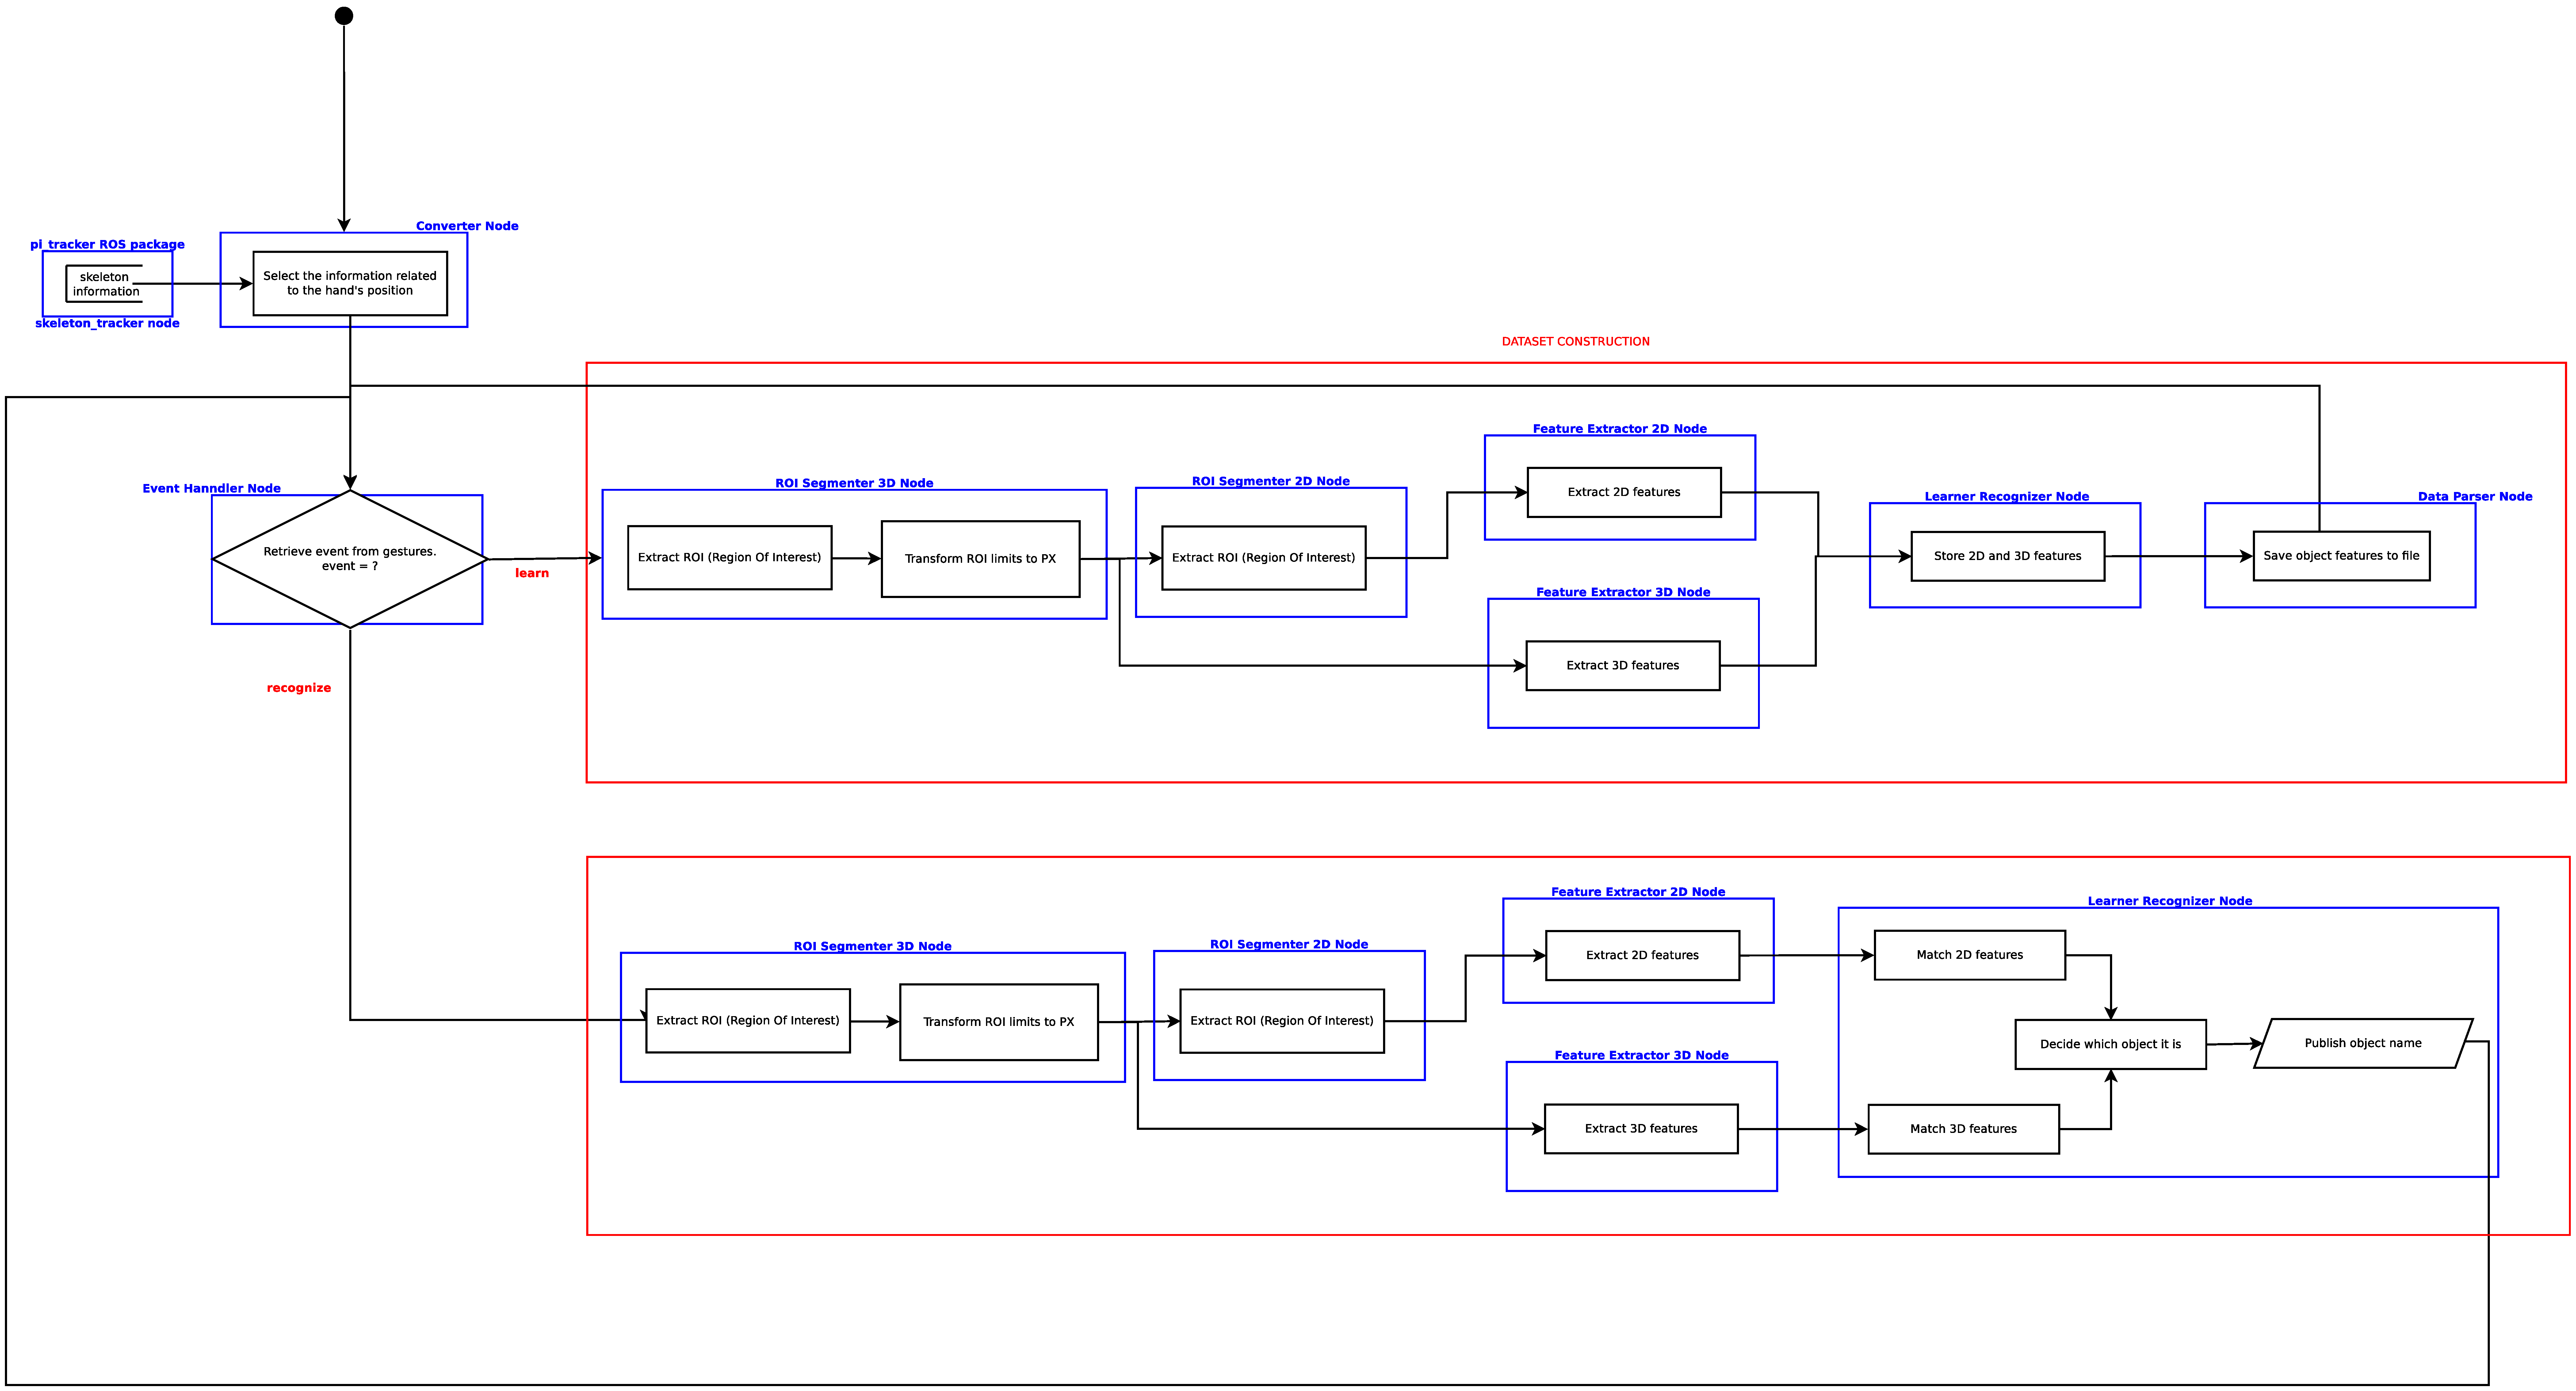
\includegraphics[scale=0.3]{img/diagrams/flowcharts.eps}
	\caption[Software flowchart]{Complete Software flowchart showing the different processing steps between the input and the output}
	\end{center}
\end{figure}


In order to fulfill those requirements a gestural interface was designed. It is developed by a separate node so the processing lags will not affect the recognition of the different gestures. This fact also allows an easy change of the gestures being used. 
\\

The recognition of the location of the hand with respect to the user's body shows how the arm is positioned. If it is stretched towards the sensor, the software enters the dataset construction mode, i.e. the data acquisition and learning mode. If, otherwise, it is located closer to the body, the software starts the object recognition mode. 
\\


The upper part of the diagram shows the data acquisition work-flow. The first step is to extract the ROI (Region of Interest) from the input raw data. This is a crucial step that allows to reduce noticeably the amount of time due to computation reducing the size of the processed information. 
\\

After the extraction, the 2D and 3D features of the segmented data are obtained. The features or descriptors are characteristics that define and represent the data from where they were created. There are different algorithms that perform this task with better or worse repeatability and robustness. All the details about this process is explained in the next chapters. 
\\

That is the end of the data cycle of the learning process. It is iterated over the number of views for each object that is required in order to obtain all the templates necessary per object. 
\\

The recognition mode was triggered when the hand was located near the user's body. This mode can be seen in the lower part of the previous diagram. 
\\

The steps that compose this part of the software are the following: 
First, the input information is converted to the custom message used within the code. Afterwards, as in the previous mode, the Region Of Interest is segmented from both 2D and 3D original information. Then, the descriptors are extracted exactly the same way as in the previous mode. 
\\

The next step is the recognition algorithm. This matches the descriptors from both the image and the point cloud and decides which object of the dataset is more similar to the one that is currently on the user's hand. More details about this algorithm may be found in this section. 
\\

Finally, the object identification number is obtained. This data is the output of the system. 


\newpage
\subsection{Third party libraries that process the input data to the system}
\label{ros_packages}
In this section the ROS packages that are used in our system are presented. 
All of them are used for the initial processing of the data coming from the RGB-D sensor. 
The connection between them and the developed nodes are explained in this section and in section \ref{nodes}.

\subsubsection{ROS package: openni\_camera}
\label{openni_camera}

This package implements the RGB-D sensors drivers.
% It is needed to connect the kinect to the computer. 
% The package is composed of nodes that perform different tasks and publish the results in topics. 
% As an example, a node transforms the raw output information of the kinect into a data array for further processing. 
The package transforms the input raw data coming from the kinect into structured one. 
This information is prepared hence for further processing. 
Figure \ref{diagram_kinect_data} shows the Connectivity graph of this package and its position in the RGB-D sensor data processing chain. 
 
 		\begin{figure}[H]
			\begin{center}
			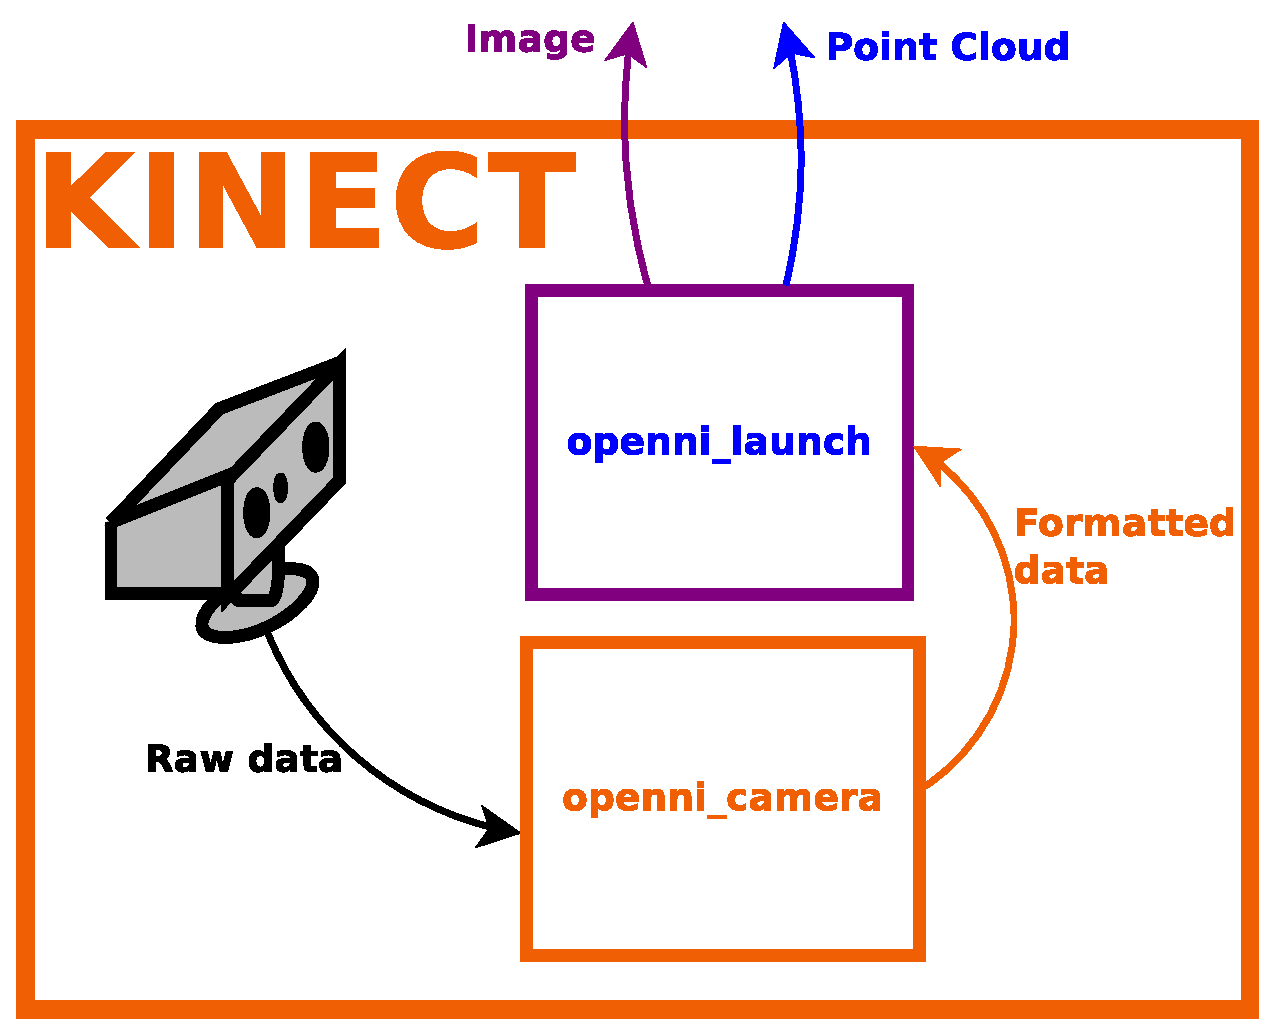
\includegraphics[width=0.5\linewidth]{img/diagrams/kinect_data.eps}
			\caption[Kinect data processing]{Kinect data processing using the openni ROS packages (openni\_camera and openni\_launch).}
			\label{diagram_kinect_data}
			\end{center}
		\end{figure}


\subsubsection{ROS package: openni\_launch}
\label{openni_launch}

This package provides useful transformations taking as input the openni\_camera topics. %and a launch file that executes nodelets with that information. 
It is composed of various nodes that can be executed using a launch file. 
Each node processes the raw input information from the driver into more useful data. 
This data may be a point cloud with color information or a disparity image for example. 
The output of the nodes is published into different topics. 
% The developed nodes described in section \ref{nodes} are subscribed to these topics in order to obtain the input point cloud and image. 
These topics are the input for the nodes that have been developed for this thesis.

\subsubsection{ROS package: pi\_tracker}

This ROS package implements a joint tracker.
It is used within the system to determine the position and orientation of the user's joints. 
This task is performed by the skeleton tracker node.  
Figure \ref{diagram_skeleton} shows the Connectivity graph of this node. 
% In figure \ref{diagram_skeleton} it may be observed that the diagram presented in figure \ref{diagram_kinect_data} is simplified.  

		\begin{figure}[H]
			\begin{center}
			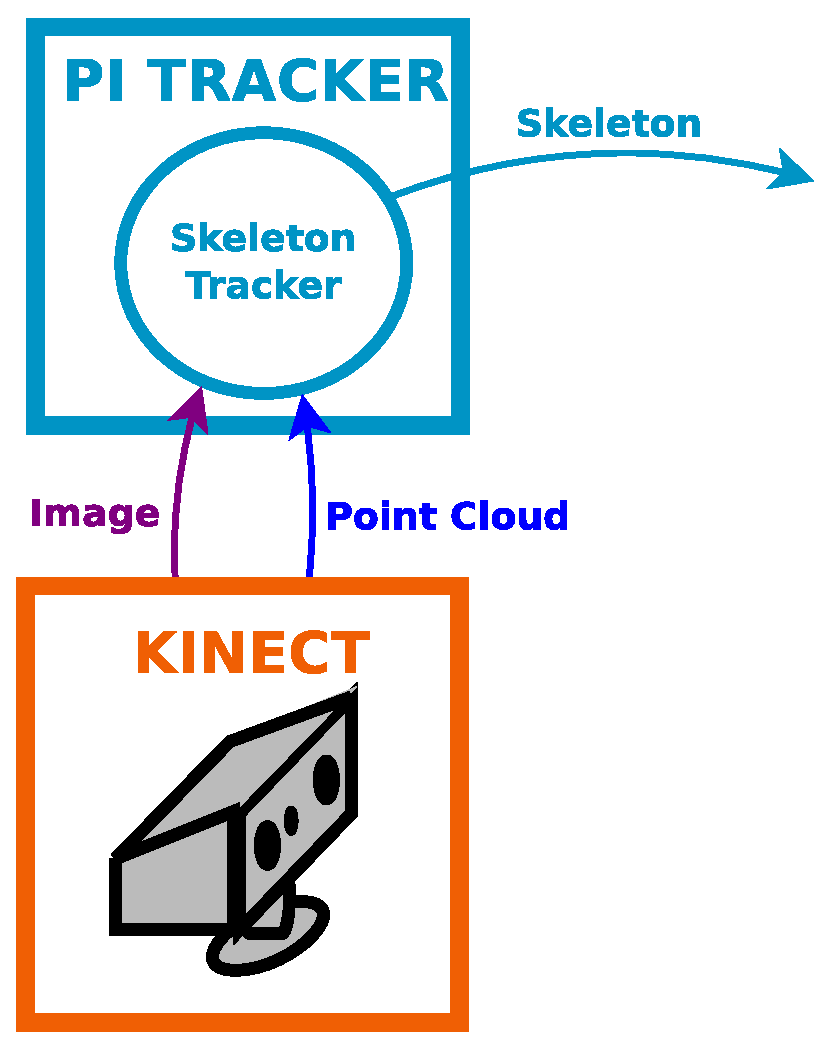
\includegraphics[width=0.3\linewidth]{img/diagrams/node_pi_tracker.eps}
			\caption[Skeleton Tracker I/O]{Connectivity graph of the Skeleton Tracker node.}
			\label{diagram_skeleton}
			\end{center}
		\end{figure}

It can be seen that the node takes as input the output data of the openni\_launch ROS package. 
The node outputs the Skeleton message in which the positions and orientations of the joints are represented. 



%\newpage
%%%%%%% SOFTWARE NODES %%%%%%
%\addcontentsline{toc}{subsection}{Software nodes}
\subsection{Description of the developed nodes}
\label{nodes}


The processing of the system is divided in nodes. 
Figure \ref{nodes_graph} shows the graph of the nodes that have been developed for the project.
% First the ones using the raw input data to the system and afterwards the ones that deliver the output of the system are described.
The circles represent the nodes. %Each circle is a node and the name inside them is the one being used in the software. 
The arrows show the communication between nodes. 
The names next to the nodes' interconnections are the messages interchanged.  % that those processes interchange. 
% The squares with the names serve as separators of the different packages that are being used. 
The square areas define the different ROS packages that have been used.
The square with the tile "OCULAR" separates the nodes developed in this thesis from third-party nodes. 
% All the nodes inside the square with the title "OCULAR" are the ones I developed. 
Sections \ref{converter} to \ref{last_node} present the processing performed by each node. 
\\


		\begin{figure}[H]
			\begin{center}
			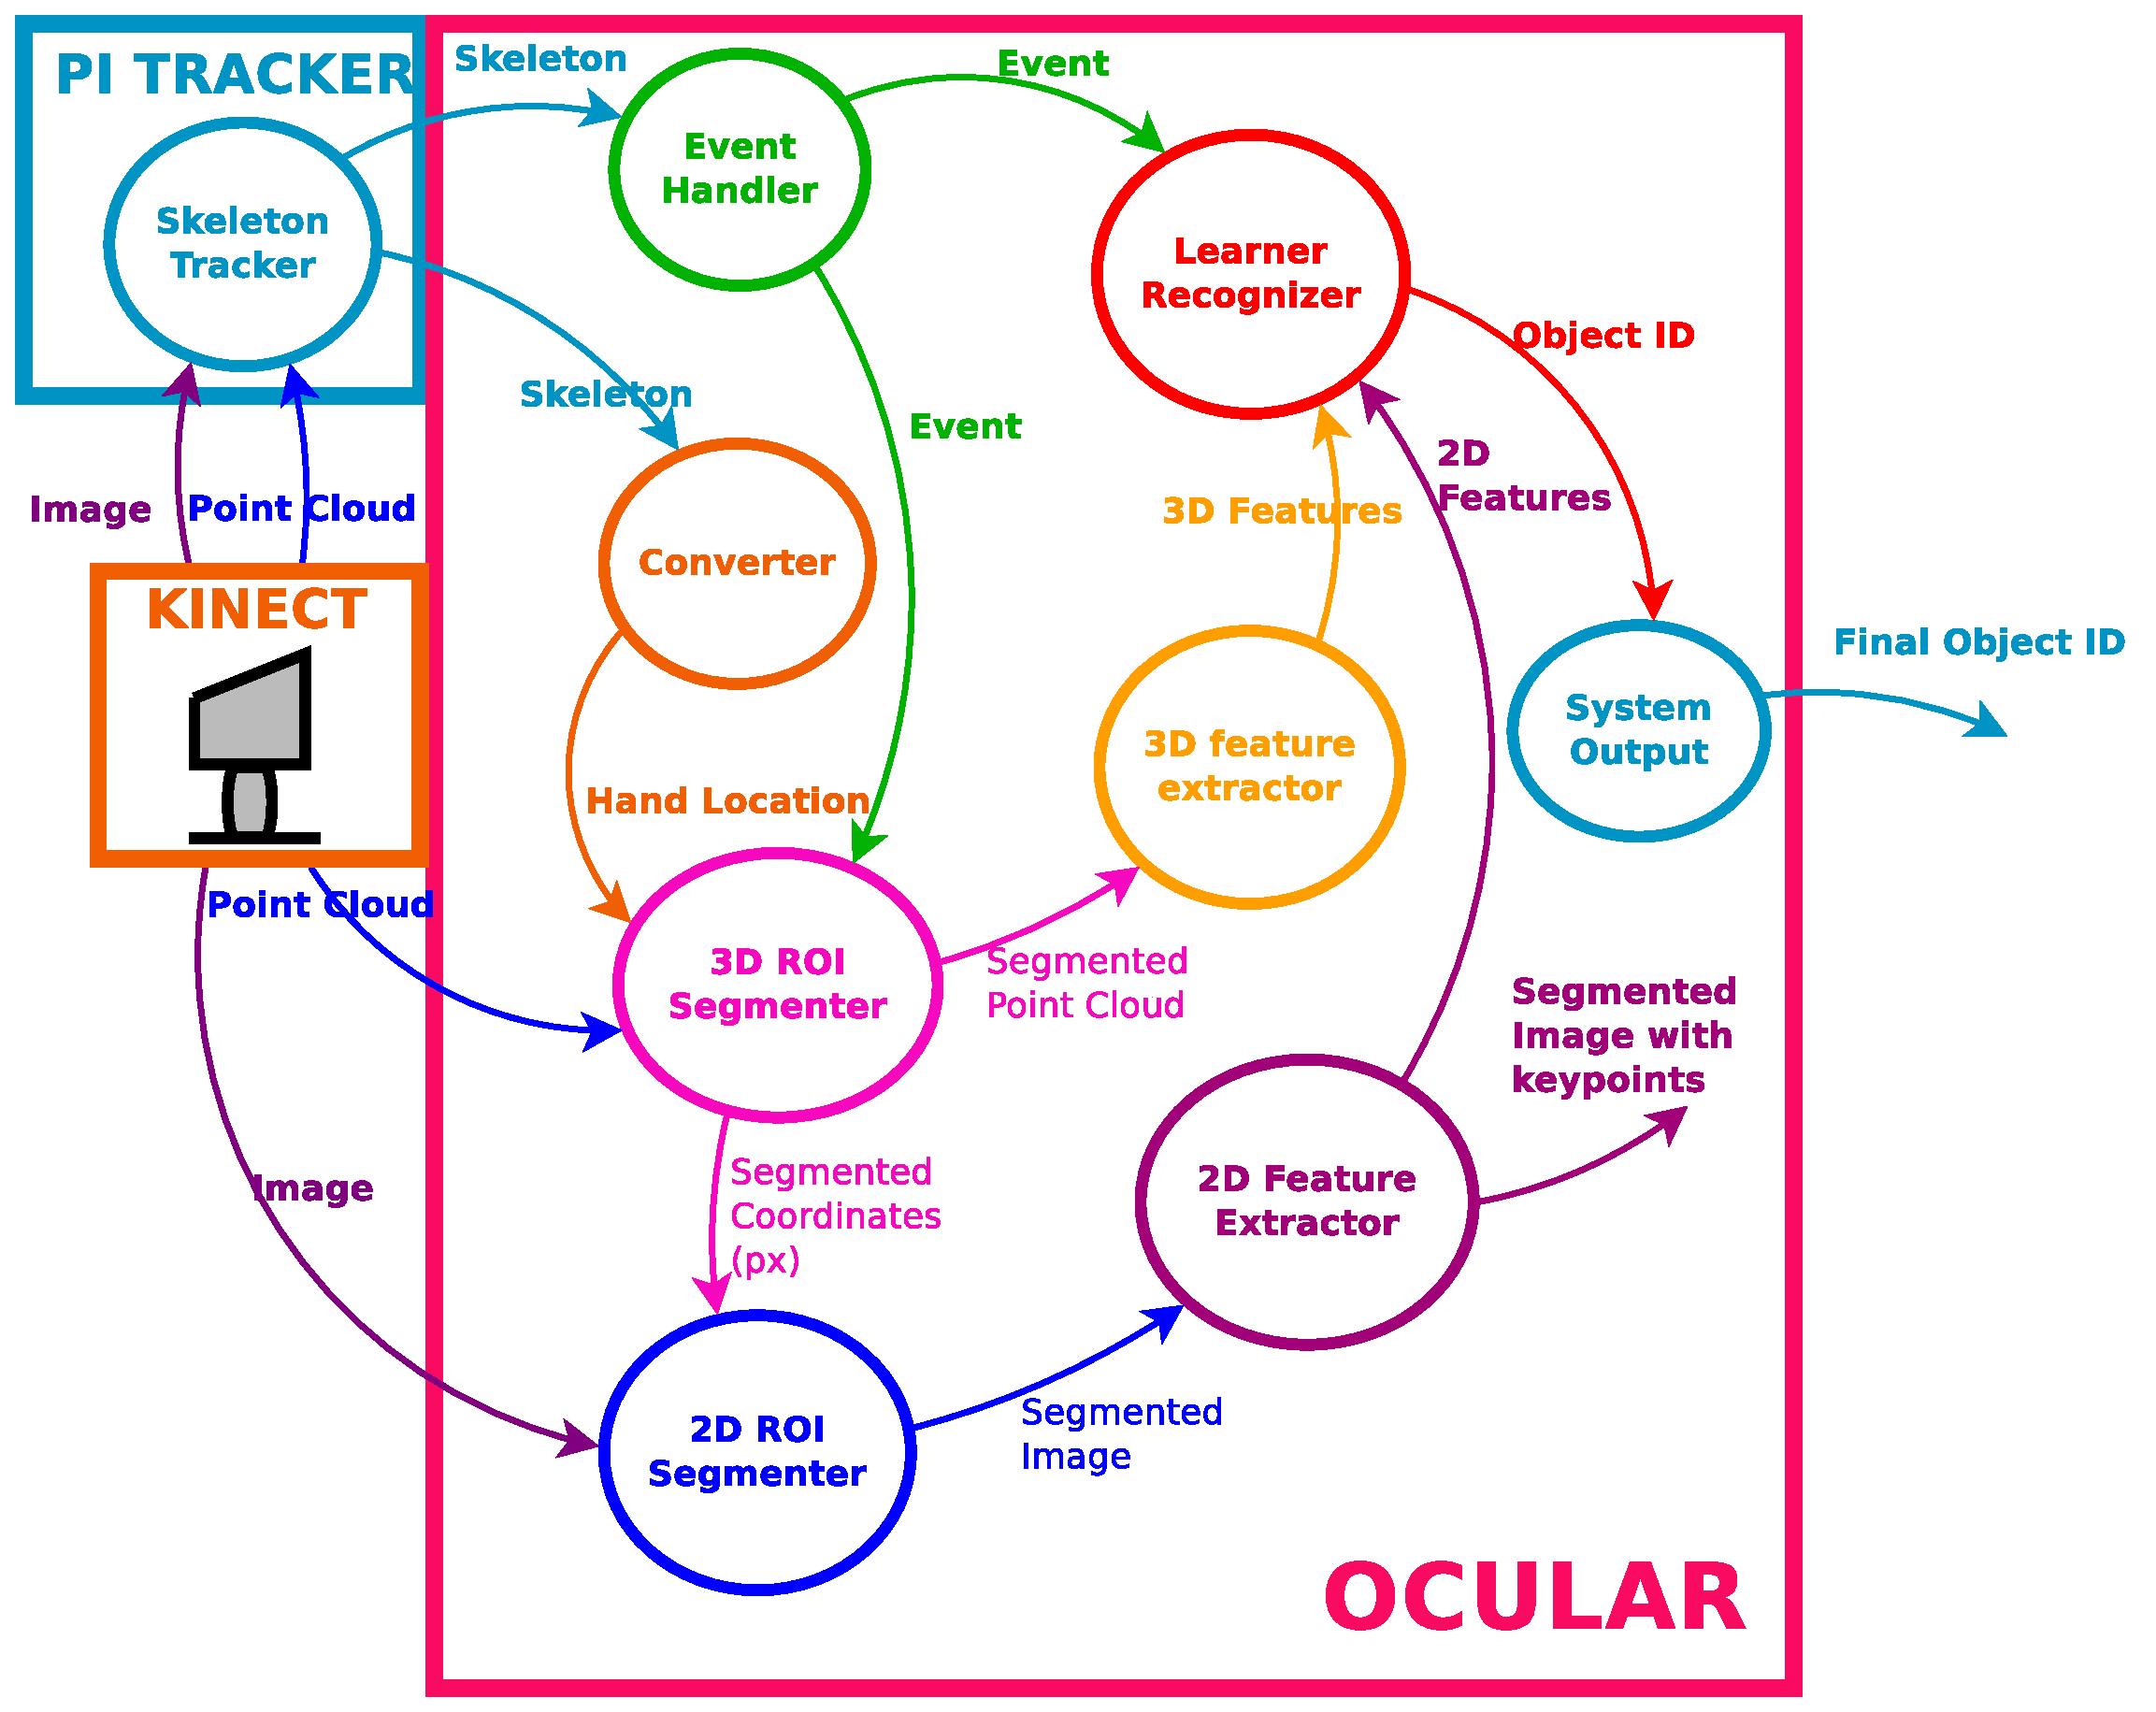
\includegraphics[width=\linewidth]{img/diagrams/nodes.eps}
			\caption[System nodes]{System nodes and their interaction.}
			\label{nodes_graph}

			\end{center}
		\end{figure}

%\newpage



%%\newpage


\subsubsection{Converter node}
		\label{converter}

	This node is the first step of the developed software. 
	It converts the input data containing the skeleton position to a custom message used through the rest of the code. 
	It allows to easily change the package from which the skeleton is obtained without affecting the whole system. 
	The converter node transforms the input data from the pi\_tracker package into the custom message used within the software. 
	It was only implemented a converter for the pi\_tracker package, but it could be easily developed a converter for other packages that retrieve the skeleton position. 
	Figure \ref{node_converter} represents the Connectivity graph of the node. 
	The skeleton message enters the node and the custom message containing the hands location is the output. 

		\begin{figure}[H]
			\begin{center}
			\includegraphics[width=0.5\linewidth]{img/diagrams/node_converter.png}
			\caption[Converter node I/O]{Connectivity graph of the Converter node.}		
			\label{node_converter}
			\end{center}
		\end{figure}

	% The information provided by that third-party code contains the position in the space of each joint of the body. 
	% The converter node takes only both hand's position. 
	The use case diagram of the node can be seen in figure \ref{uc_converter}. 

	\begin{figure}[H]
		\centering
		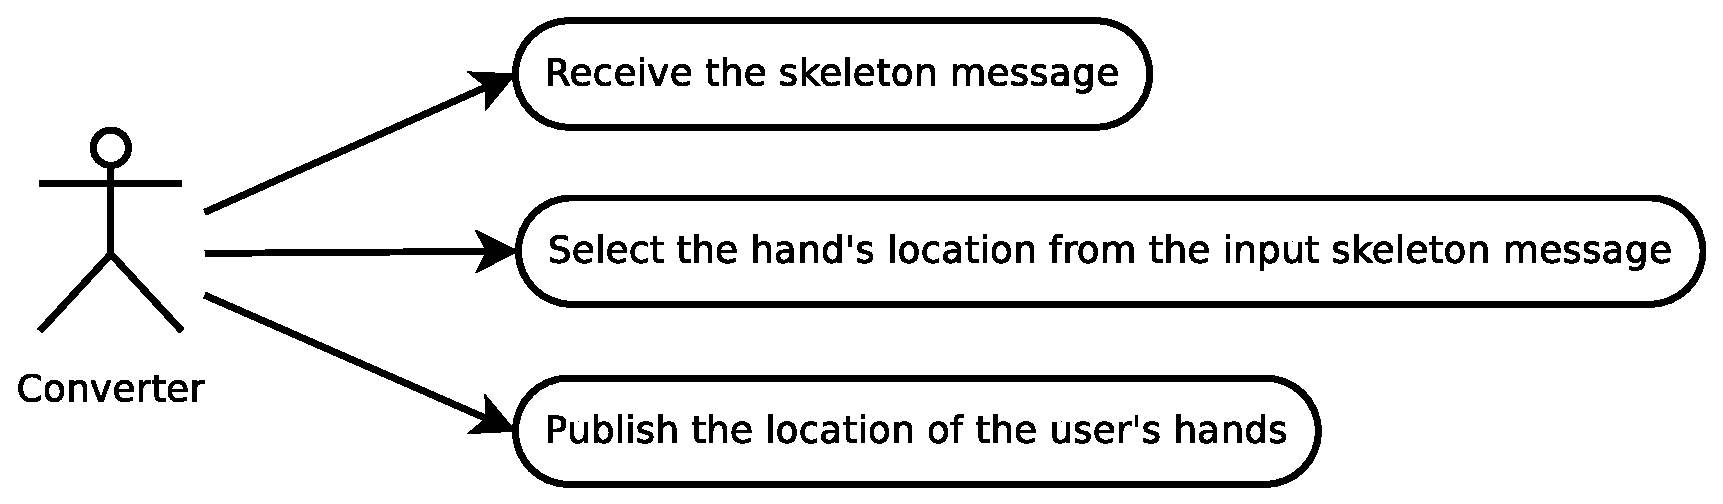
\includegraphics[scale=0.4]{img/diagrams/uc_converter.eps}
		\caption[Use case diagram converter node]{Use Case diagram of the converter node}
		\label{uc_converter}
	\end{figure}

	
	%%\newpage

\subsubsection{3D ROI Segmenter node}
	\label{roi_segmenter_3d}

	Figure  \ref{node_roi3d} presents the Connectivity graph of the node. 
	The input of this node is the raw 3D information from the sensor and the hand's locations from the third-party package pi\_tracker, as well as the hand in which the user is holding the object. 

		\begin{figure}[H]
			\begin{center}
			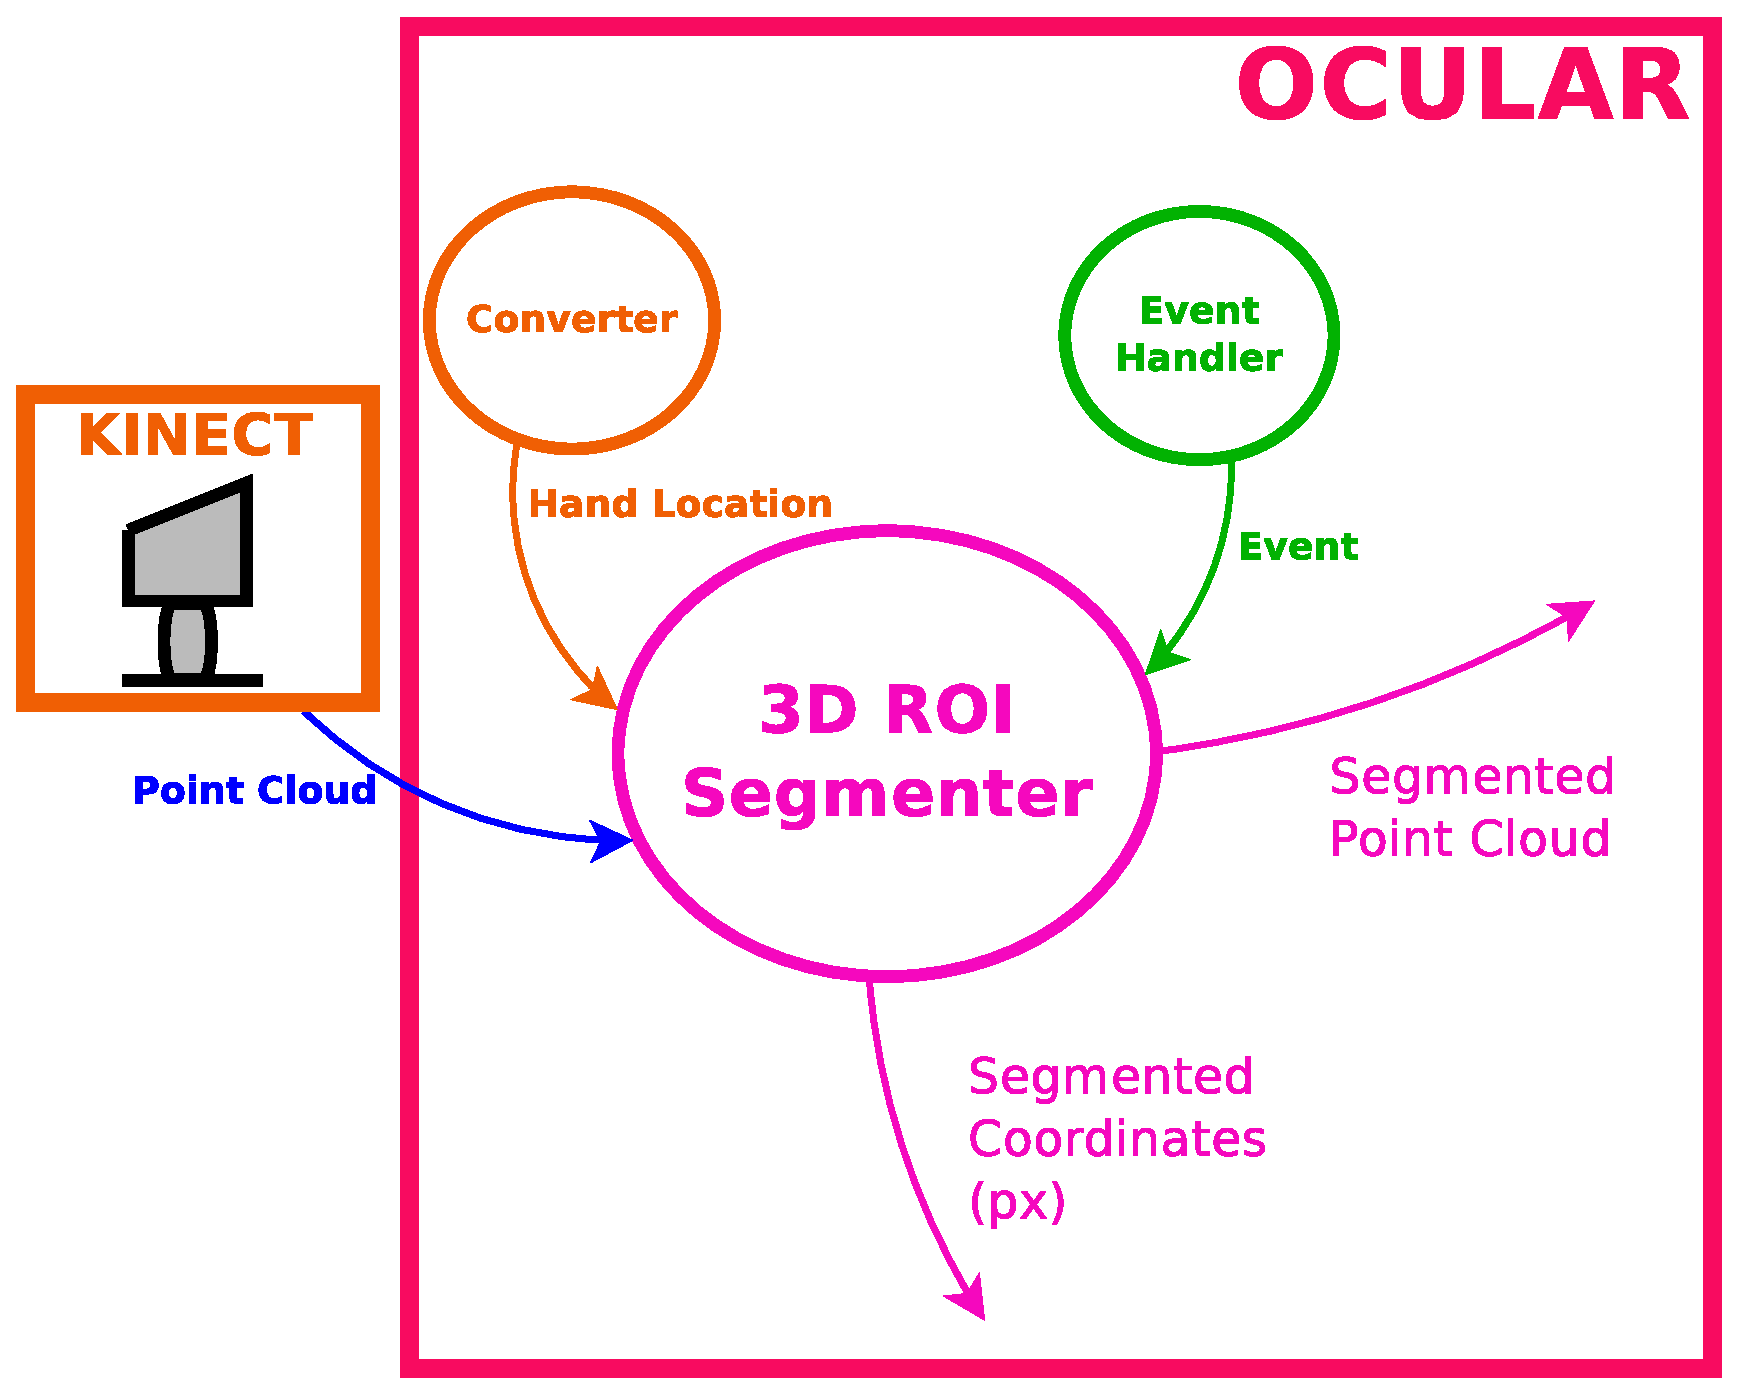
\includegraphics[width=0.5\linewidth]{img/diagrams/node_roi3d.eps}
			\caption[ROI segmenter 3D node I/O]{Connectivity graph of the ROI segmenter 3D node.}		
			\label{node_roi3d}
			\end{center}
		\end{figure}


	The node segments a prism from the original point cloud around the selected hand's center. 
	The prism vertex coordinates are transformed from world coordinates to pixels. 
	This is done to allow the ROI Segmenter 2D to perform the cropping of the input image using those pixel values. 
	That information is the output of the node, together with the segmented point cloud. 
	Figure \ref{uc_roi3d} shows the use case diagram of the node. 

	\begin{figure}[H]
		\centering
	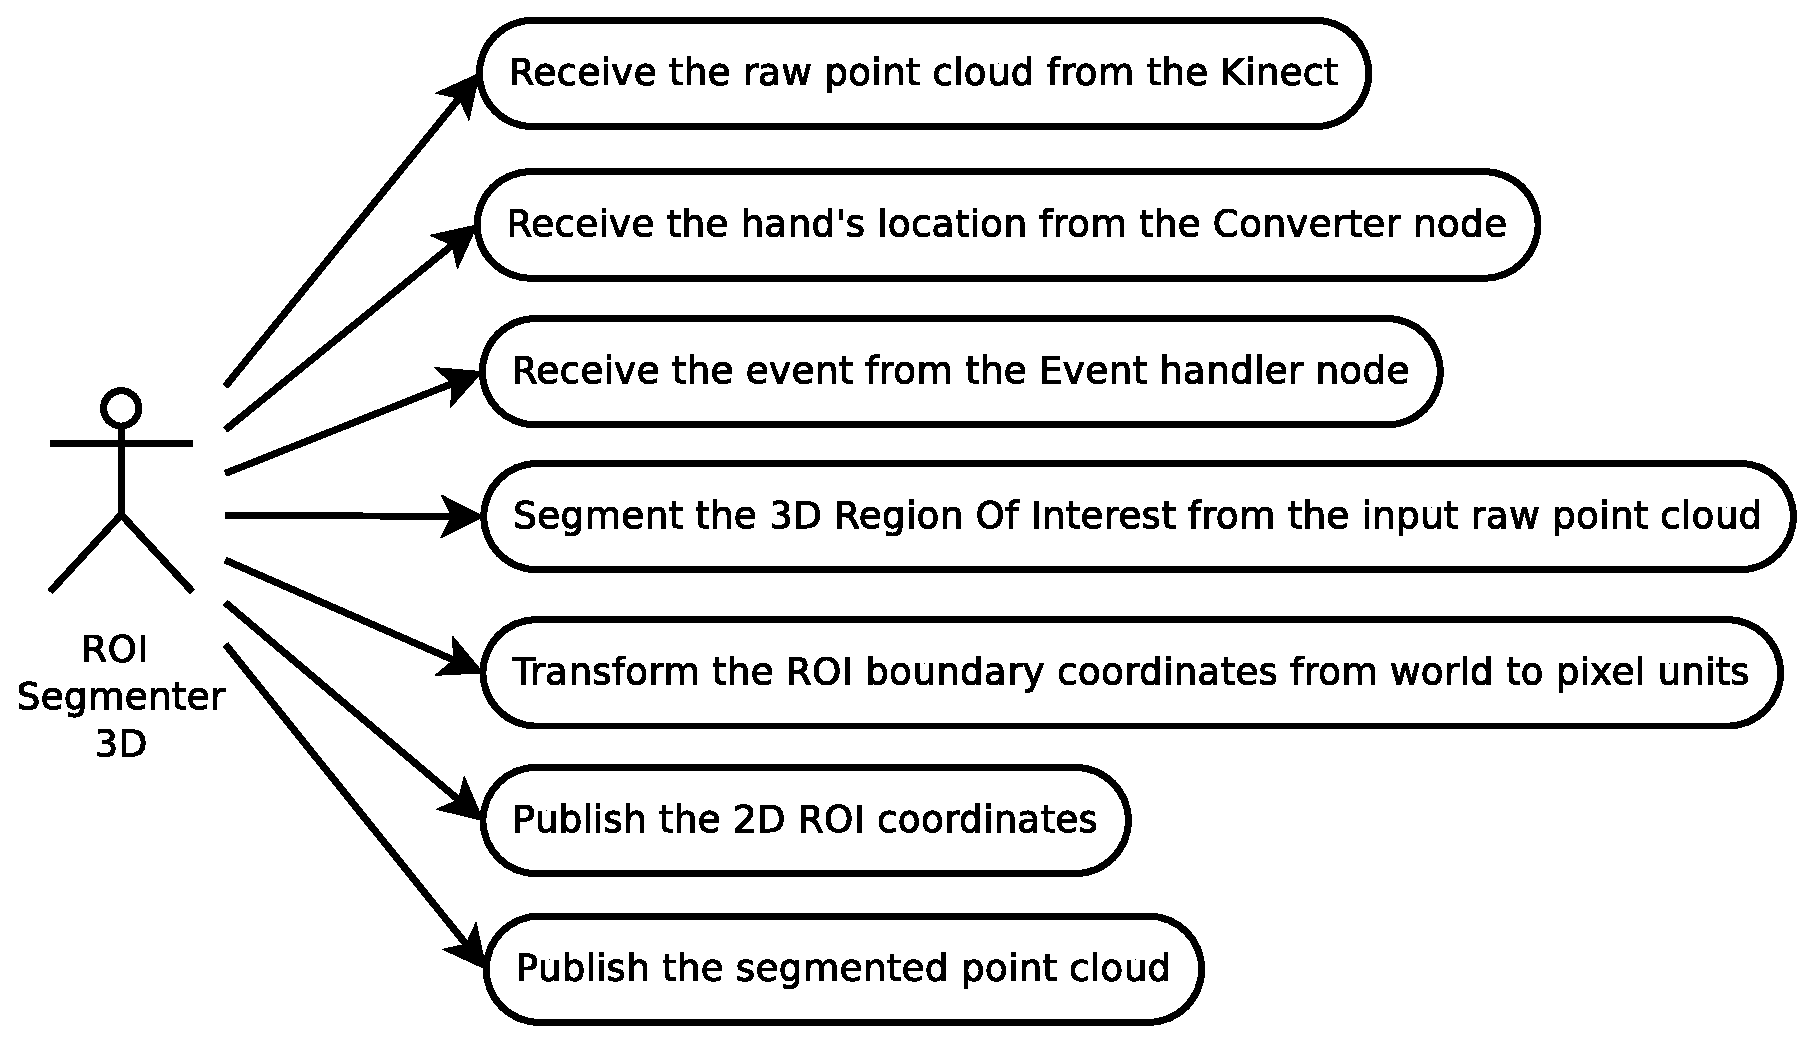
\includegraphics[scale=0.4]{img/diagrams/uc_roi_segmenter_3d.eps}
		\caption[Use case diagram ROI segmenter 3D node]{Use Case diagram of the ROI segmenter 3D node}
		\label{uc_roi3d}	
	\end{figure}
 
%%\newpage

\subsubsection{2D ROI Segmenter node}
	\label{roi_segmenter_2d}
	
	%The present node takes as the input the raw 2D information from the RGB-D sensor and the hand's locations in pixels returned from the ROI segmenter 3D node. 
	Figure \ref{node_roi2d} depicts the Connectivity graph of this node. 
	The raw 2D information and the hand location in pixels are inputs to the ROI Segmenter 2D node. 

		\begin{figure}[H]
			\begin{center}
			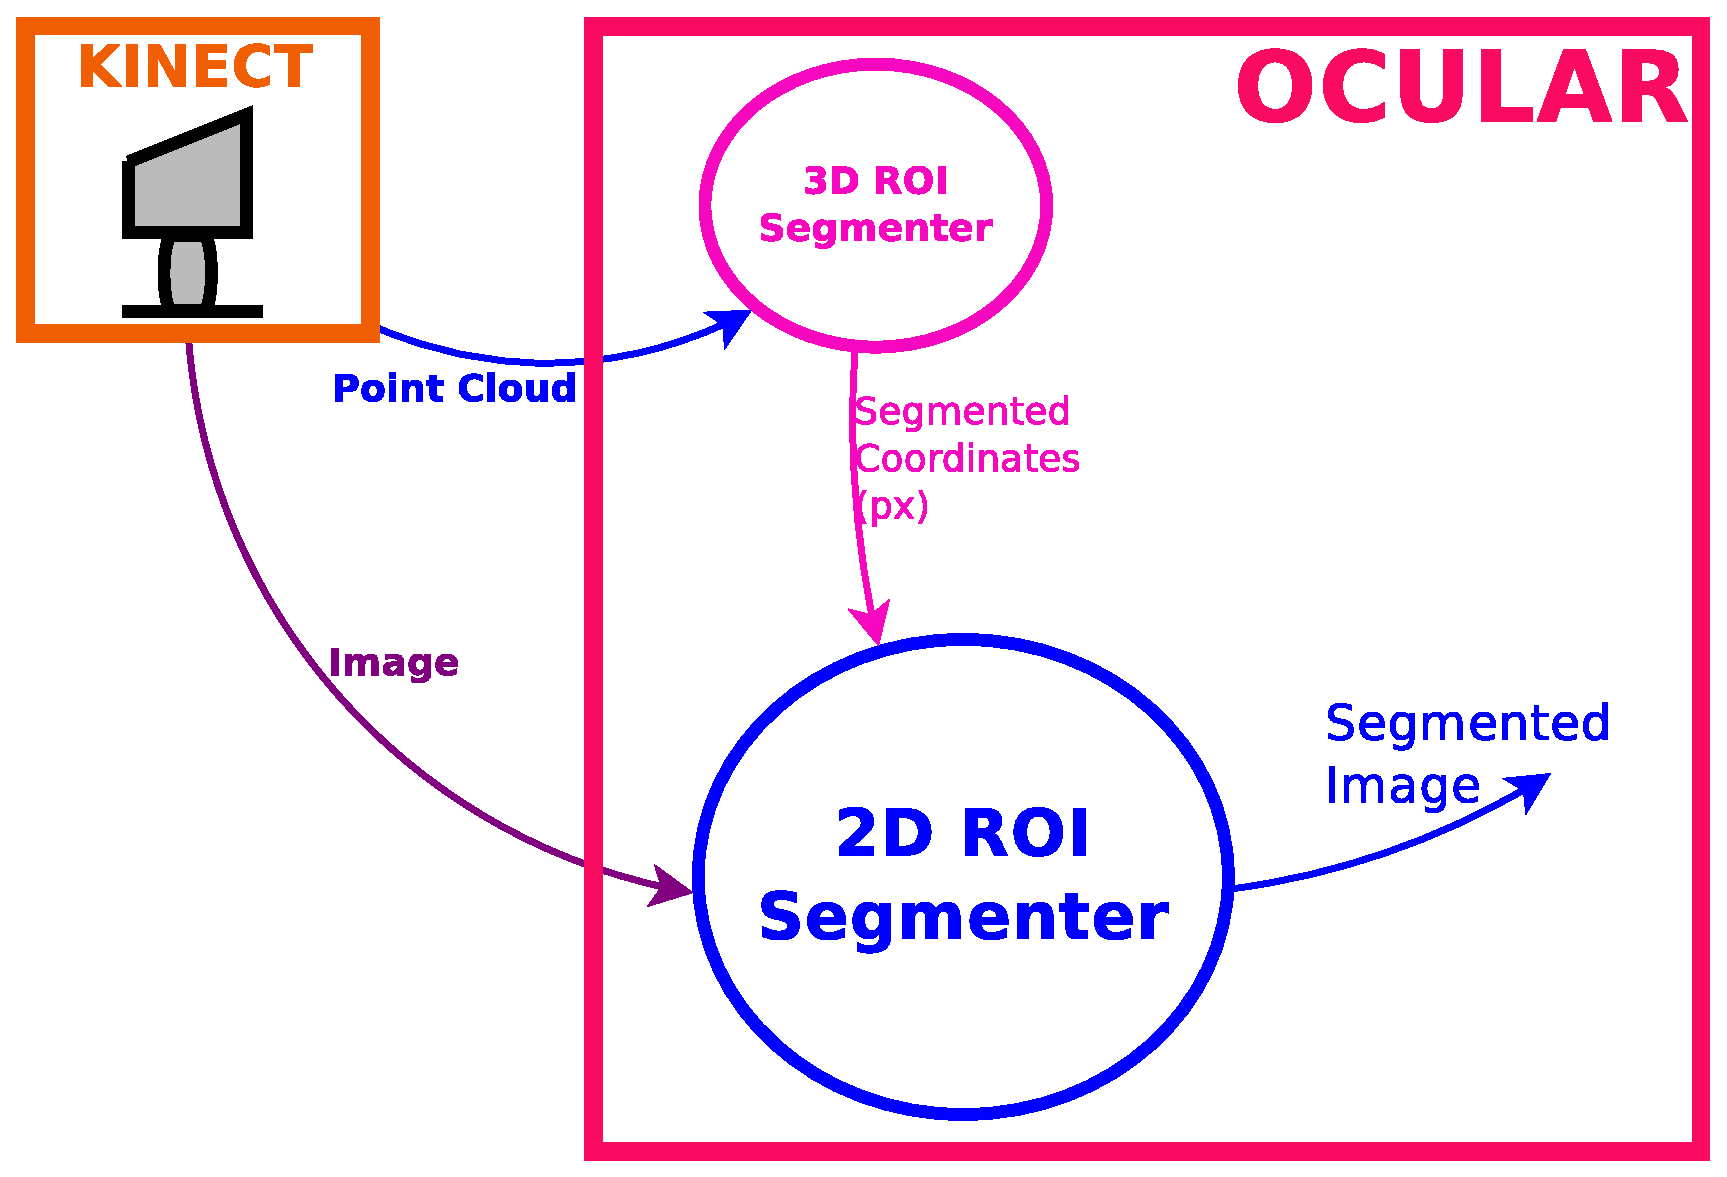
\includegraphics[width=0.5\linewidth]{img/diagrams/node_roi2d.eps}
			\caption[ROI segmenter 2D node I/O]{Connectivity graph of the ROI segmenter 2D node.}		
			\label{node_roi2d}
			\end{center}
		\end{figure}

	The processing performed is the following: First, the ROI (Region Of Interest) is cropped taking a square section around the center of the hand. 
	The size of that figure is fixed for simplicity. 
	This fact does not affect the segmentation since the difference in the scale in negligible in the operating range of the system. 
	The range is determined by the skeleton tracker node and also the low resolution of the RGB-D sensor. 
	The system may be used at a distance between 1.5m and 2.5m. 
	%Since due to the RGB-D sensor's current resolutions the user must remain at a fixed distance from the sensor, the difference in the scale due to the distance is negligible and hence the size can be fixed. 
	\\
	In figure \ref{uc_roi2d} the use case diagram of the node can be observed.
	\begin{figure}[H]
		\centering
			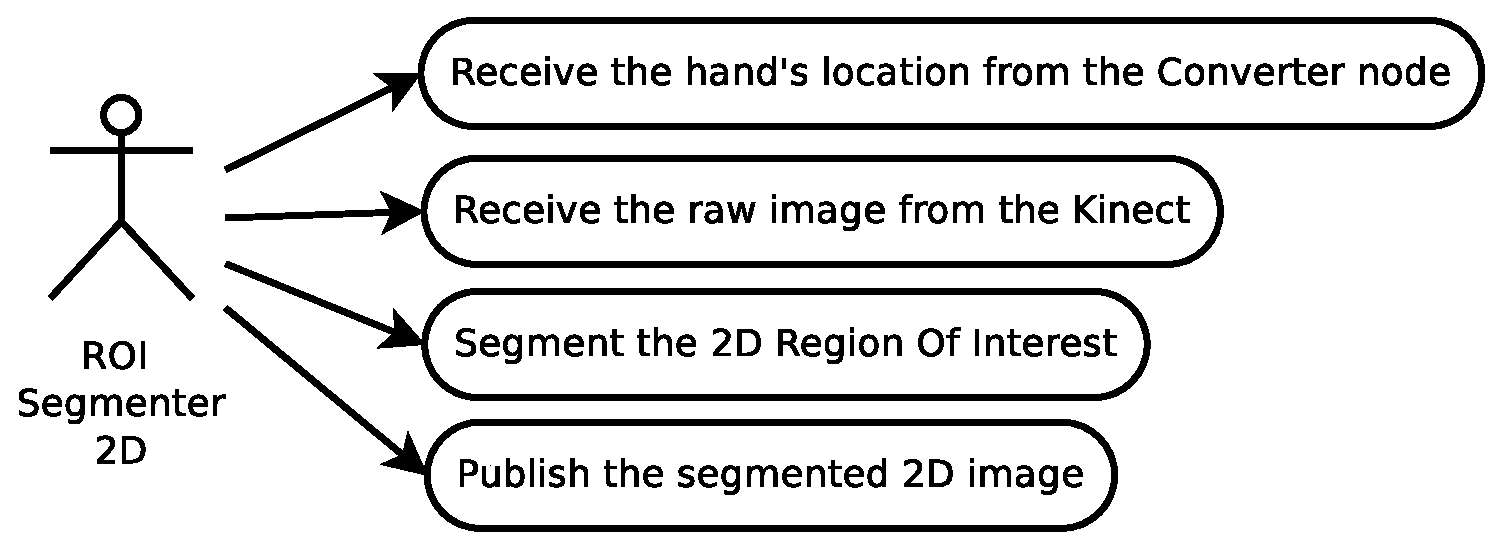
\includegraphics[scale=0.4]{img/diagrams/uc_roi_segmenter_2d.eps}
			\caption[Use case diagram ROI segmenter 2D node]{Use Case diagram of the ROI segmenter 2D node}
		\label{uc_roi2d}
	\end{figure}

%%\newpage

\subsubsection{2D Feature Extractor node}

	This node takes as an input the segmented 2D ROI from the previous nodes and extracts the features. 
	Figure \ref{node_fe2d} shows the Connectivity graph of the node. 

		\begin{figure}[H]
			\begin{center}
			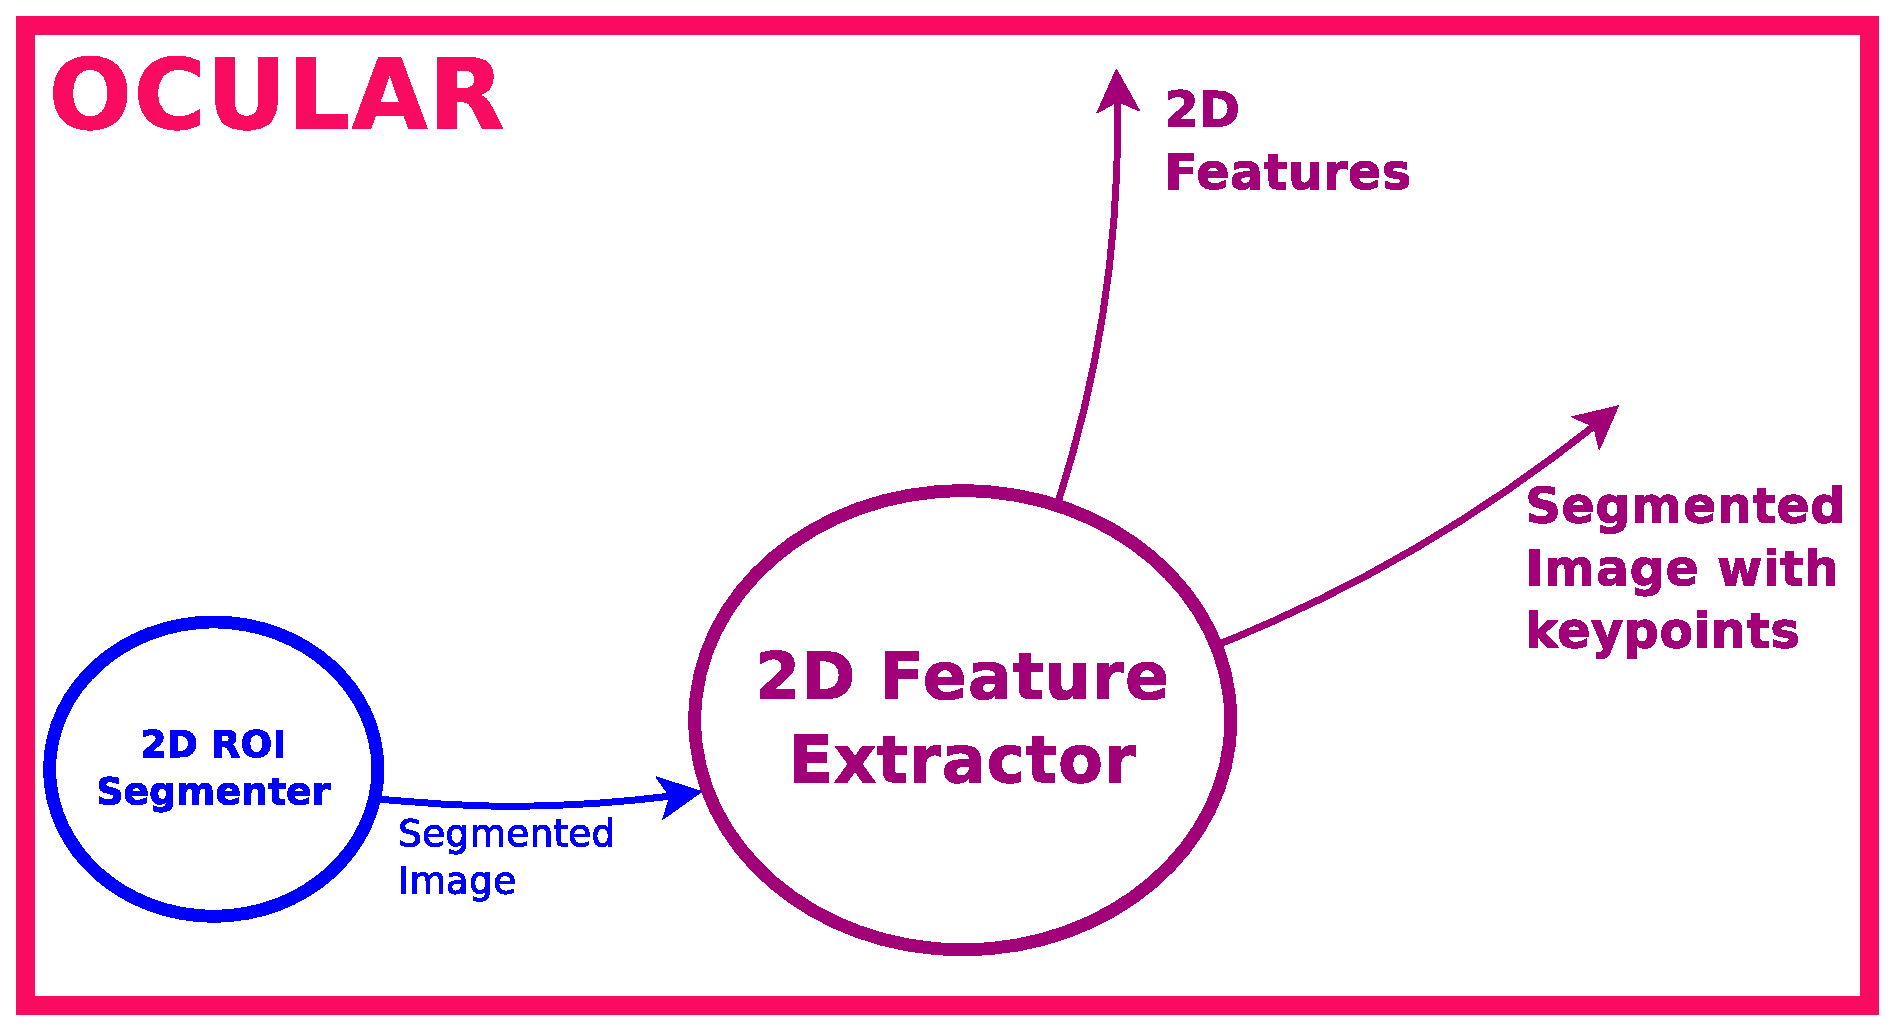
\includegraphics[width=0.5\linewidth]{img/diagrams/node_fe2d.eps}
			\caption[Feature Extractor 2D node I/O]{Connectivity graph of the Feature Extractor 2D node.}		
			\label{node_fe2d}
			\end{center}
		\end{figure}

	There are two output messages of this node, the segmented images with keypoints and the 2D ORB descriptors. 
	The descriptors matrix is the one being used in the rest of the system. 
	The segmented image with the keypoints drawn on it is outputted for debugging and development reasons. 
	\\

	Figure  \ref{uc_fe2d} represents the use case diagram of this node. 
	\begin{figure}[H]
		\centering
			\includegraphics[scale=0.4]{img/diagrams/uc_feature_extractor_2d.eps}
			\caption[Use case diagram Feature Extractor 2D node]{Use Case diagram of the Feature Extractor 2D node}
		\label{uc_fe2d}
	\end{figure}

%%\newpage

\subsubsection{3D Feature Extractor node}

	The input of this node is the segmented point cloud from the ROI Segmenter 3D node (see section \ref{roi_segmenter_3d}. The descriptors are extracted from this information and are published in the output topic. 
	\\
		\begin{figure}[H]
			\begin{center}
			\includegraphics[width=0.5\linewidth]{img/diagrams/node_fe3d.eps}
			\caption[Feature Extractor 3D node I/O]{Connectivity graph of the Feature Extractor 3D node.}		
			\label{node_fe3d}
			\end{center}
		\end{figure}

	Figure \ref{uc_fe3d} shows the use case diagram of the node. 

	\begin{figure}[H]
		\centering
			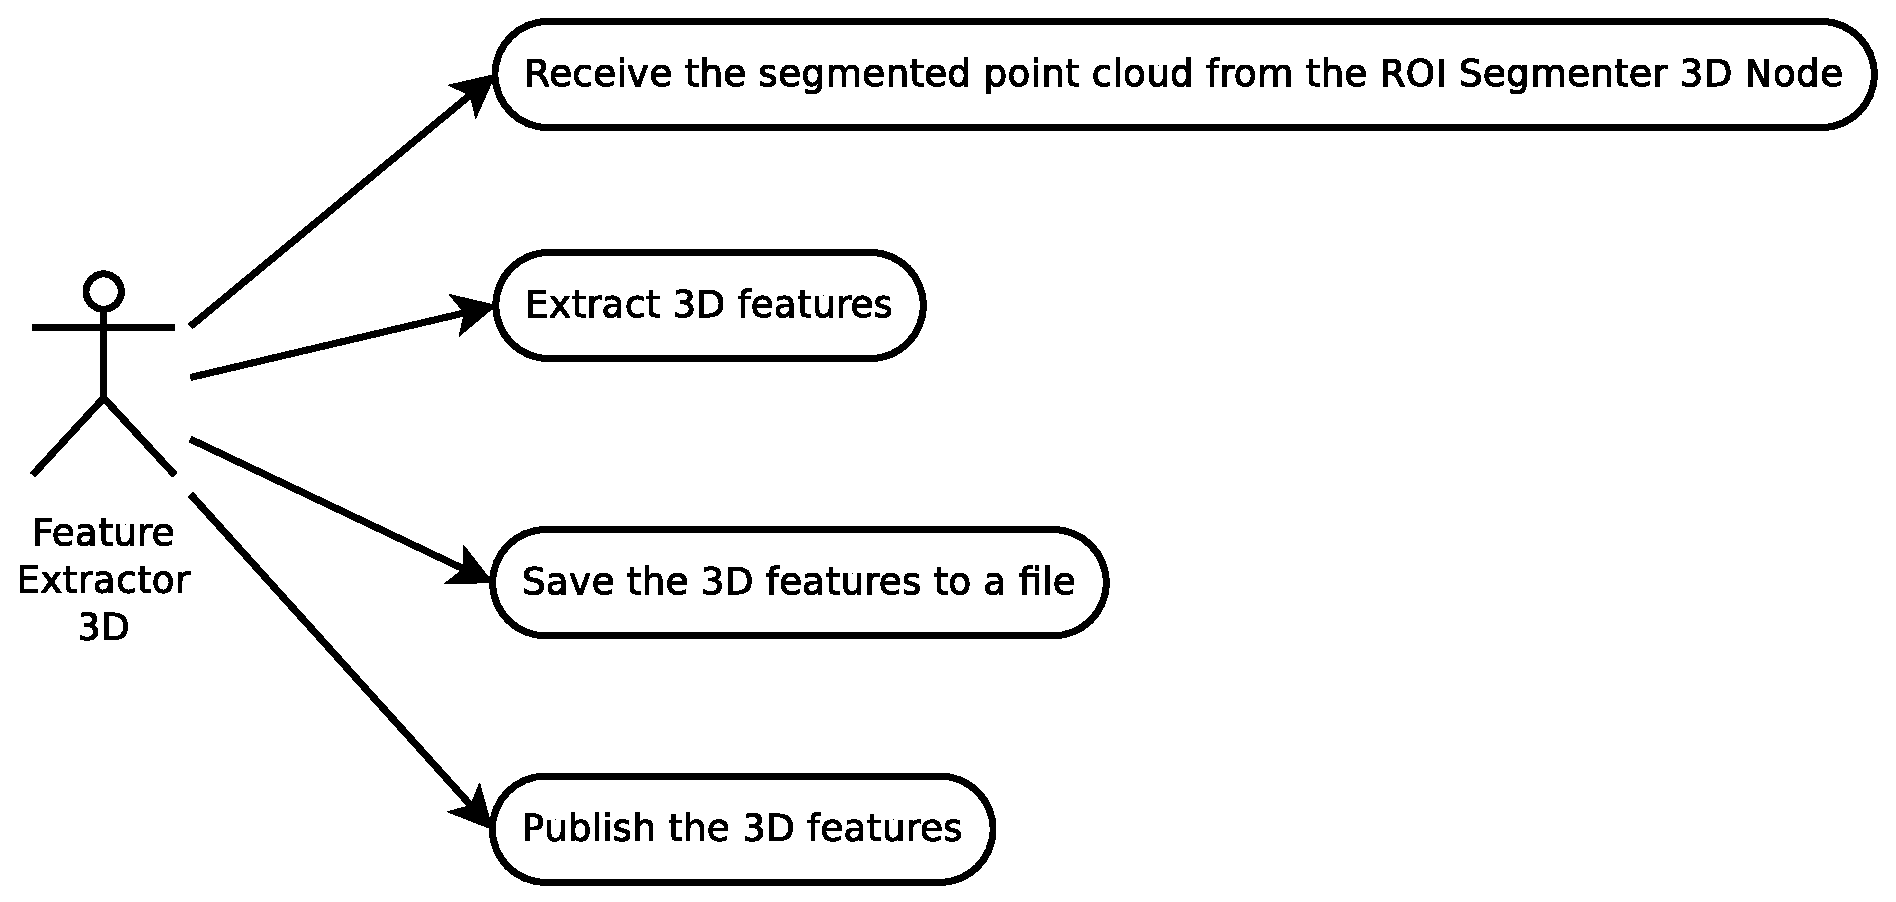
\includegraphics[scale=0.4]{img/diagrams/uc_feature_extractor_3d.eps}
			\caption[Use case diagram Feature Extractor 3D node]{Use Case diagram of the Feature Extractor 3D node}
		\label{uc_fe3d}
	\end{figure}

%%\newpage

\subsubsection{Event Handler node}

	As it was previously stated, in order to interact with the software some gestures were defined. This is the module that detects those gestures and switches accordingly to the corresponding event. This is the node responsible of detecting the different events that can appear in the system. 
	\\
	Figure \ref{node_event} shows the different Connectivity graph of the node. 
		\begin{figure}[H]
			\begin{center}
			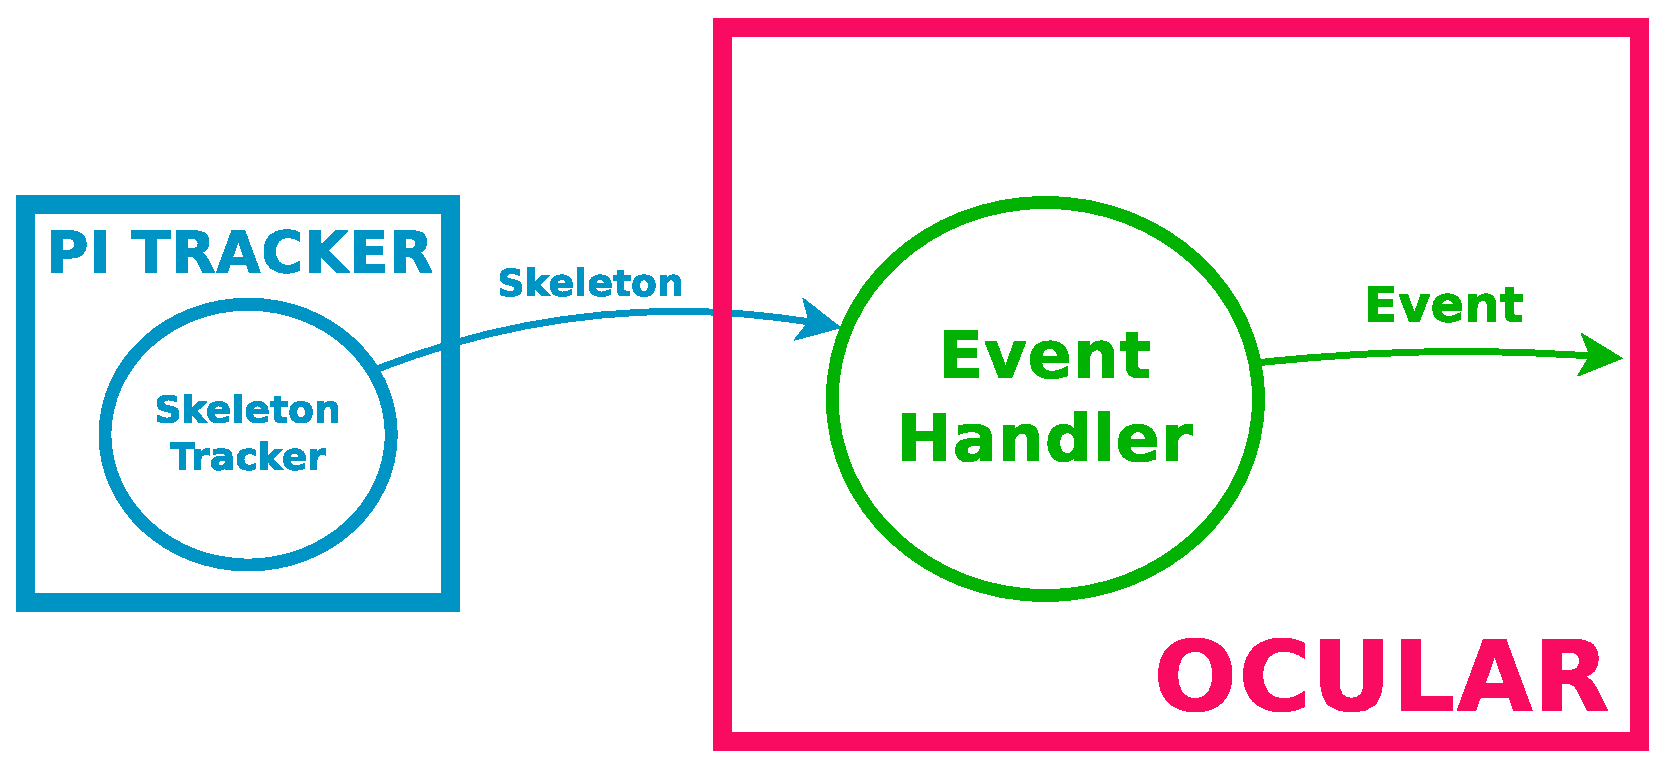
\includegraphics[width=0.5\linewidth]{img/diagrams/node_event.eps}
			\caption[Event Handler 3D node I/O]{Connectivity graph of the Event Handler node.}		
			\label{node_event}
			\end{center}
		\end{figure}
	The input of the system is the skeleton message that is obtained from the third-party package pi\_tracker. This message contains the information of all the joints of the user. The information is screened to detect the height at which each hand is located. The one that is the highest is the one being used in the software. Afterwards, the distance between the body and the chosen hand is computed. When that distance is similar to the distance of the user's arm, the event triggered is "learn". If, otherwise, the hand is located close to the body, the event that is published to the output topic is "recognize". 
	\\

	The distance that triggers the modes is proportional to the distance between the user and the RGB-D sensor in order to obtain a range of use of the software higher. 
	Figure \ref{uc_event} is a diagram with the use case of the node. 
	\begin{figure}[H]
		\centering
			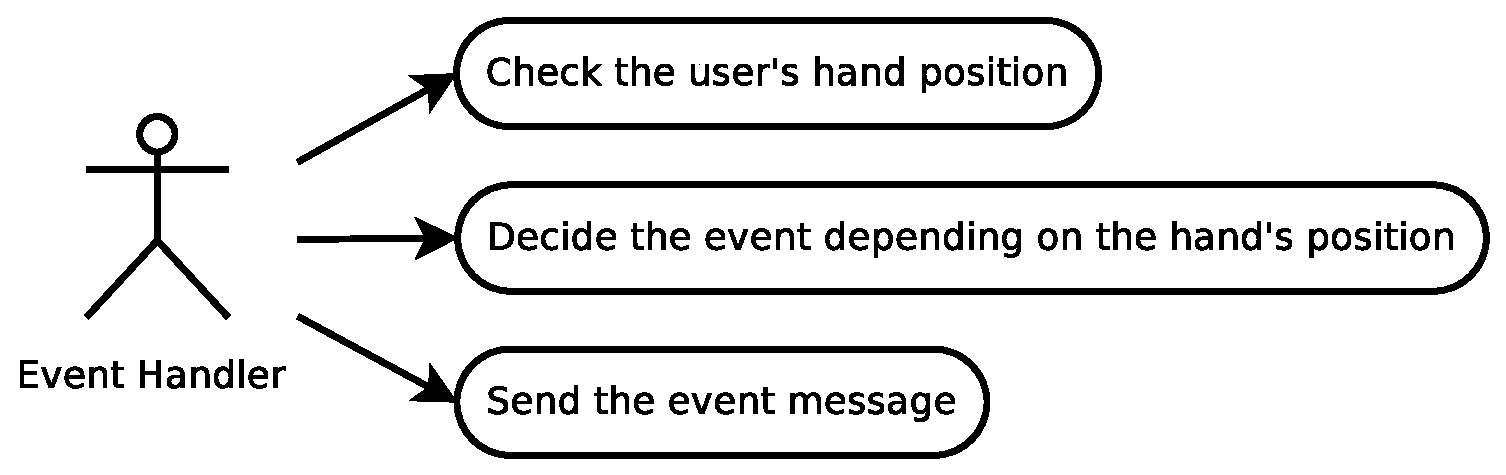
\includegraphics[scale=0.4]{img/diagrams/uc_event_handler.eps}
			\caption[Use case diagram Event Handler node]{Use Case diagram of the Event Handler node}
		\label{uc_event}
	\end{figure}

%%\newpage

\subsubsection{Learner-Recognizer node}
\label{learner_recognizer}

	This node implements the state machine depending on the events recognized by the event handler node. If the event received is "learn", the learning sequence starts. If the event is "recognize", the recognize sequence is triggered. 
	\\

		\begin{figure}[H]
			\begin{center}
			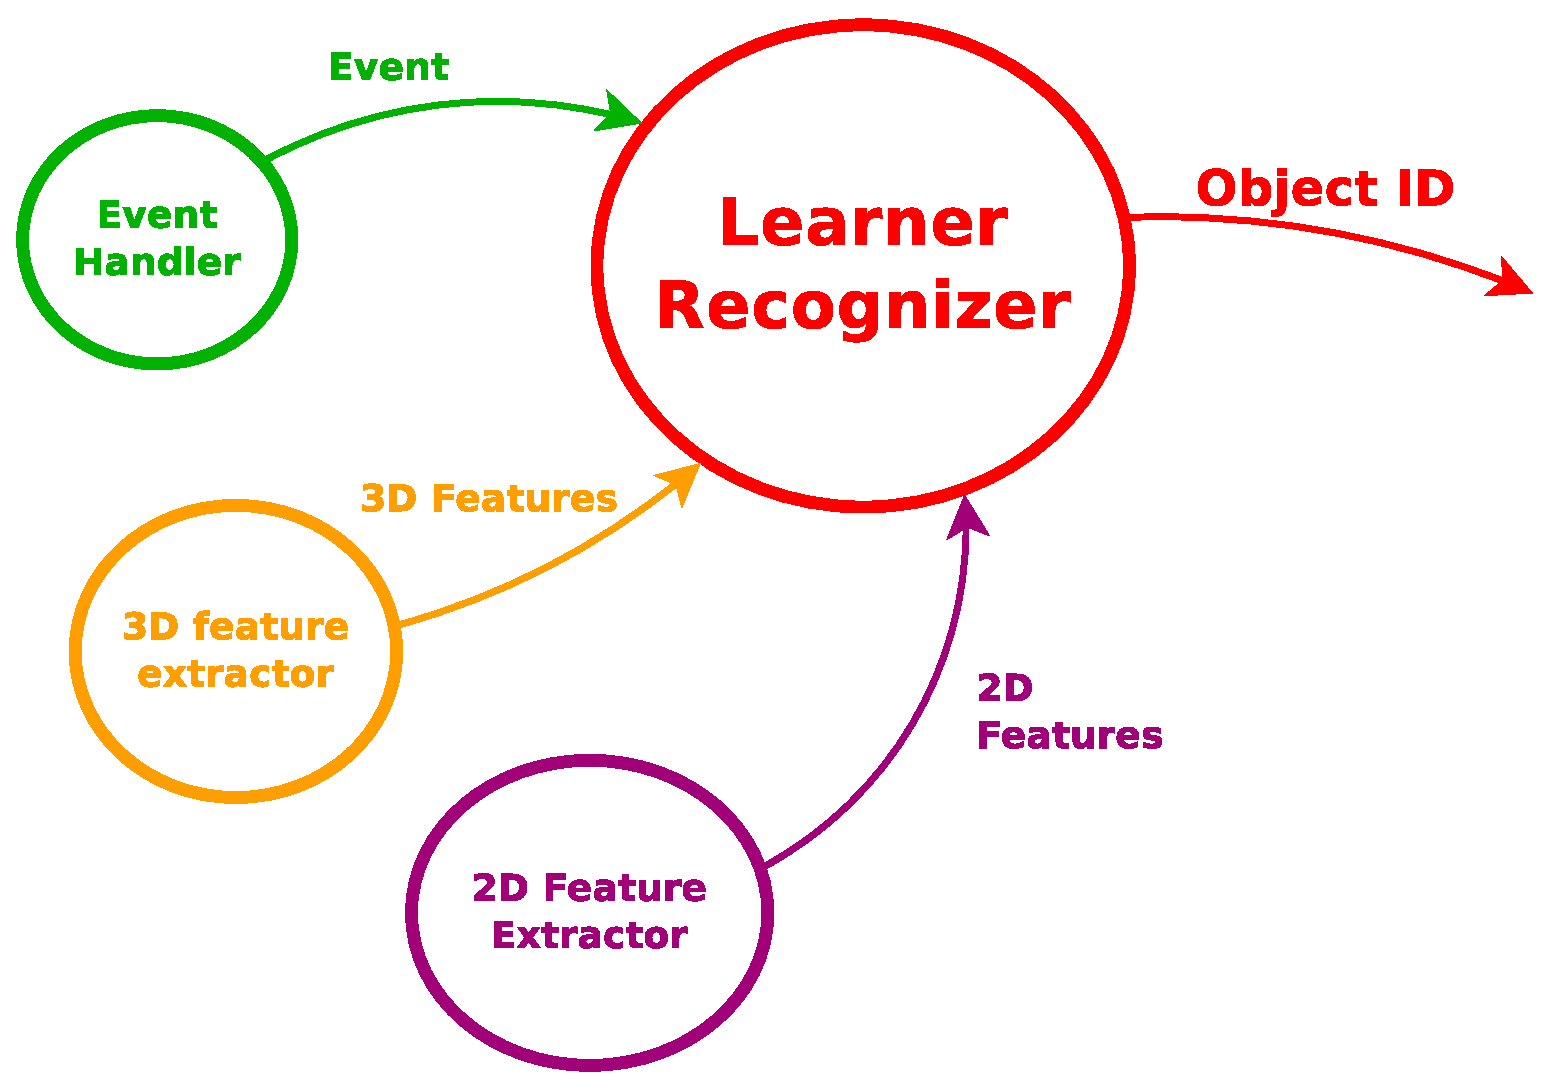
\includegraphics[width=0.5\linewidth]{img/diagrams/node_lr.eps}
			\caption[Learner-Recognizer node I/O]{Connectivity graph of the Learner-Recognizer node.}		
			\end{center}
						\label{node_lr}

		\end{figure}

	The learn sequence consists in obtaining and storing the features both 2D and 3D and waiting a second allowing the user to move the object to capture a new view of it. 
	The dataset extracted is saved to a folder when the software is closed, to prevent possible lags in the runtime of the program. 
	Each view is saved separately. 
	This node loads the files that are still in the saving folder when the program is restarted. 
	\\

	The recognition sequence compares the newly obtained features both 2D and 3D with the ones that are stored in the dataset. 
	Afterwards, the result of the recognition for both types of descriptors are published in the output topic. 
	Figure \ref{uc_learner_recognizer} presents the use case diagram of the node. 

	\begin{figure}[H]
		\centering
			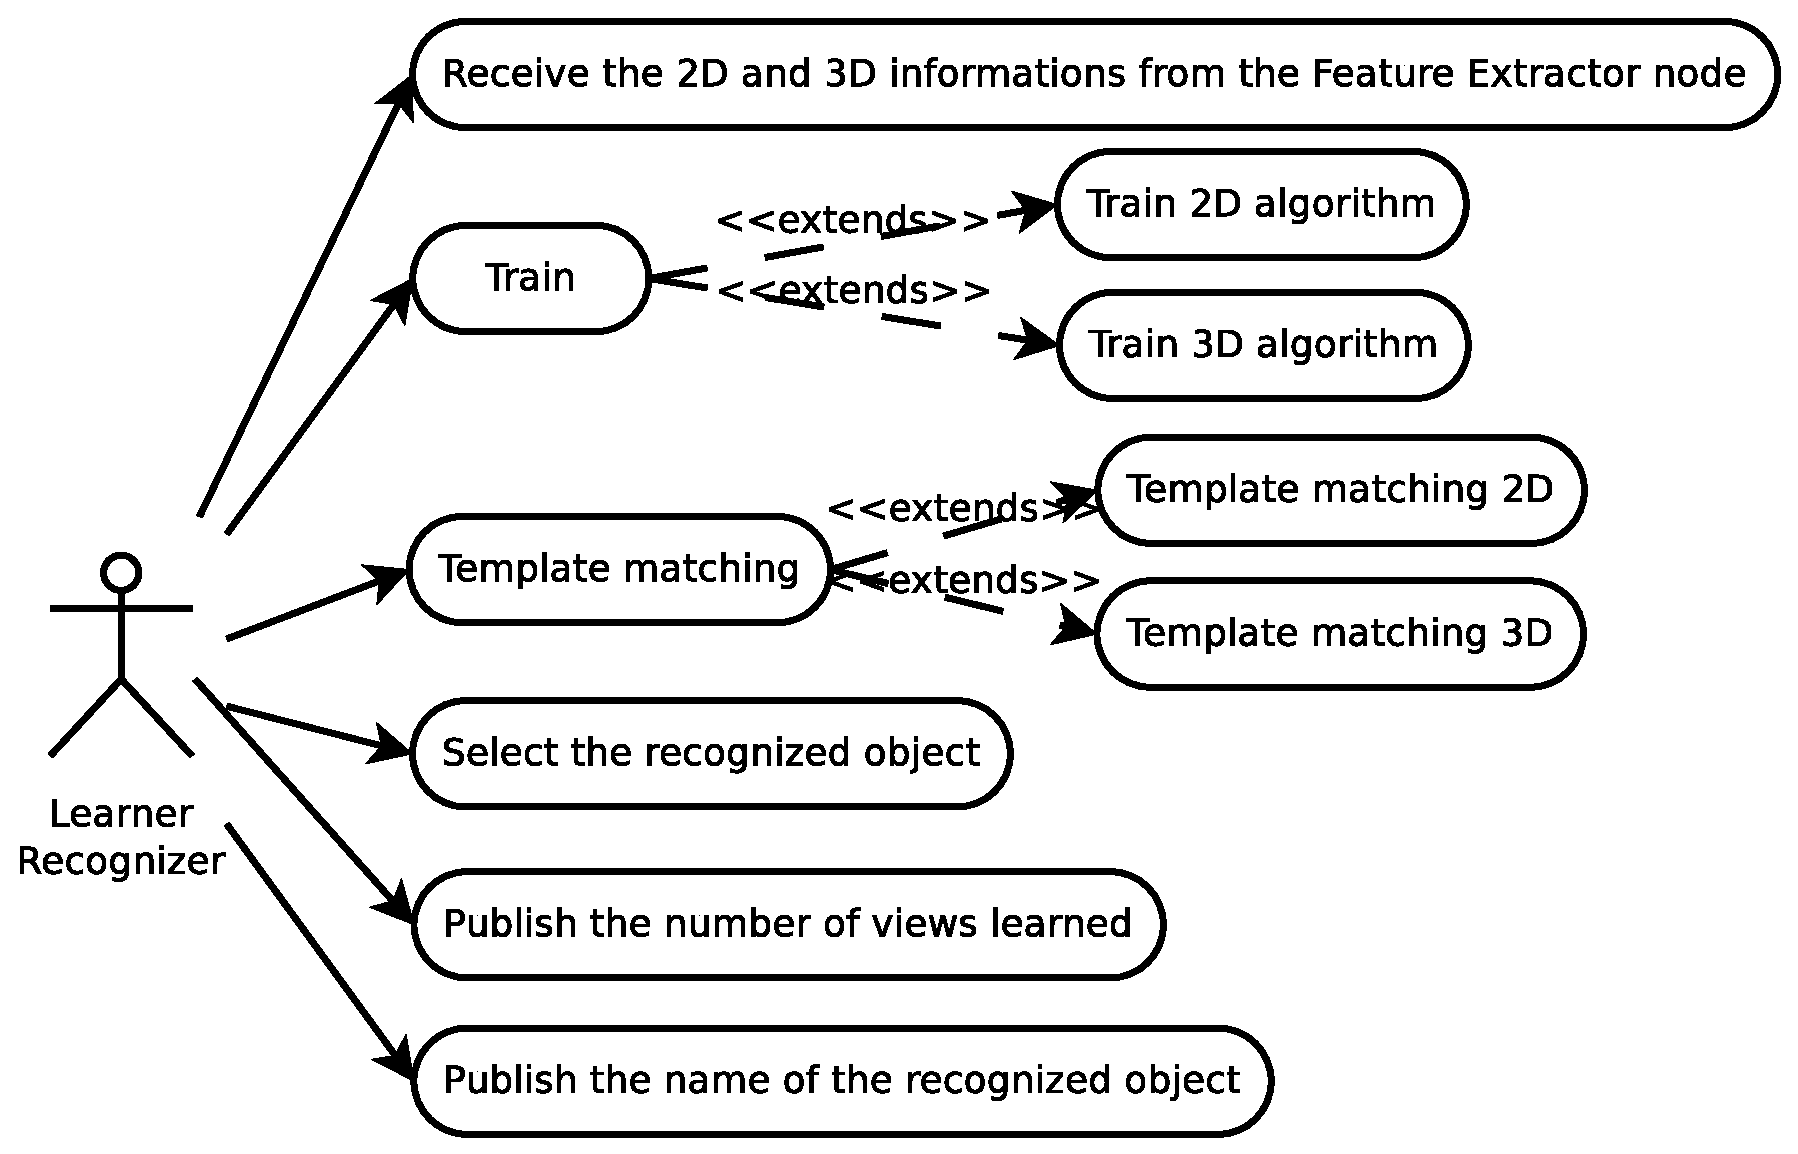
\includegraphics[scale=0.4]{img/diagrams/uc_learner_recognizer.eps}
			\caption[Use case diagram Learner-Recognizer node]{Use Case diagram of the Learner-Recognizer node}
			\label{uc_learner_recognizer}
	\end{figure}

%%\newpage


\subsubsection{System Output node}
\label{last_node}
	This nodes implements a buffer and a decision algorithm. 
	The input of the node is the object ID message from the Learner-Recognizer process as can be seen in figure \ref{node_output}.
	The node stores thirty values of instantaneous object estimations. 
	Since the Kinect runs at 30 frames per second, each second a new final object estimation appears. 
	The output of the node is the final object ID. 


		\begin{figure}[H]
			\begin{center}
			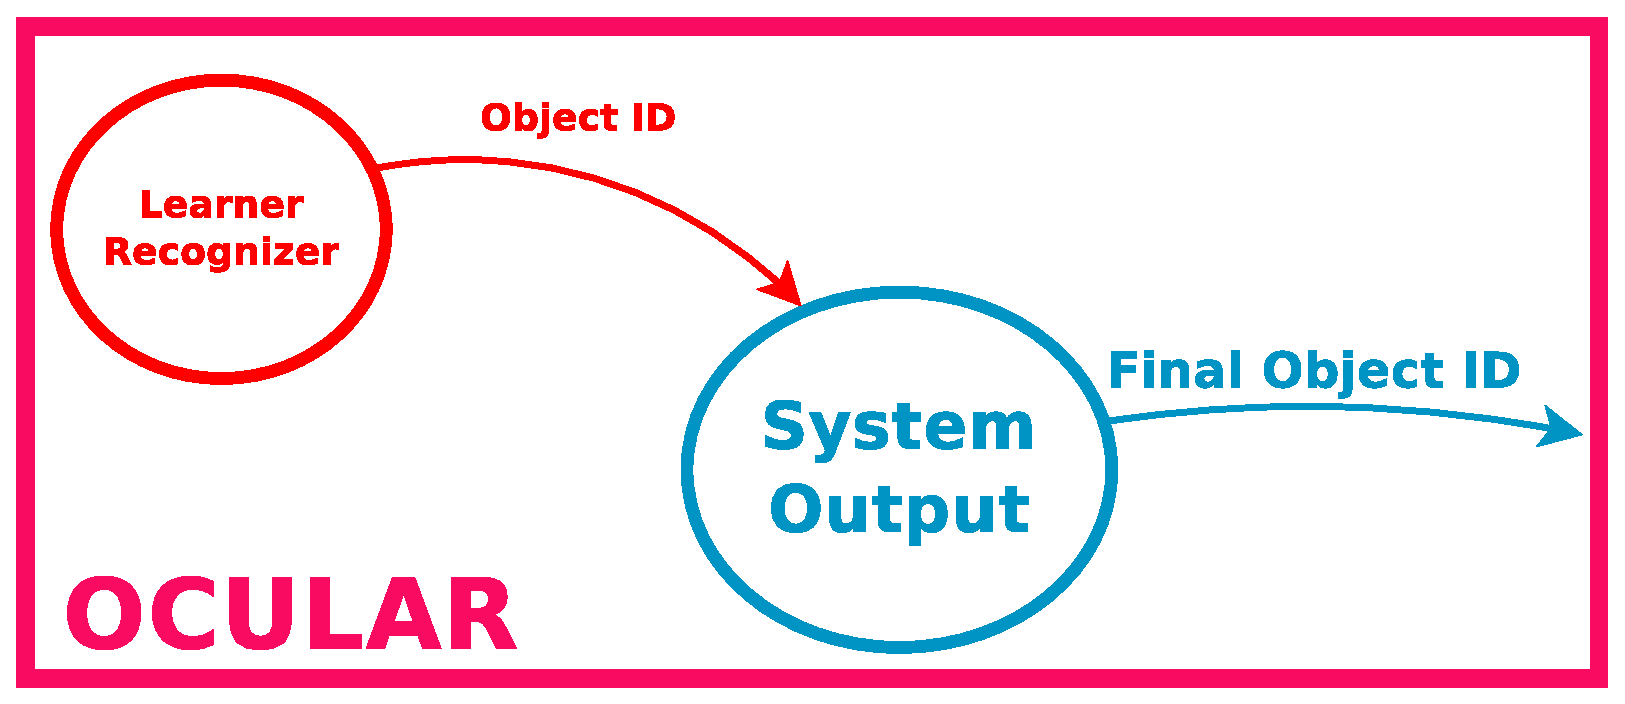
\includegraphics[width=0.5\linewidth]{img/diagrams/node_output.eps}
			\caption[System Output node I/O]{Connectivity graph of the System Output node.}		
			\label{node_output}
			\end{center}
		\end{figure}

	The decision is performed as follows. 
	The input to the algorithm are two vectors containing the 2D and 3D object estimations. 
	The frequency of each class is obtained. 
	Let us represent as $y'_{2D}$ and $y'_{3D}$ the vectors containing in each element the frequency of the object with $object_id = element$. 
	Both informations are combined in one vector called $y'$. 
	\\
	\begin{center}
	$y'=0.6*y'_{2D}+0.4*y'_{3D}$
	\end{center}
	More importance is being given to the 2D estimations since the 2D descriptors are more robust than the 3D ones. 
	The estimated final object id ($Y$) is obtained as the vector element that has the highest value. 
	\\
	\begin{center}
		$Y'= argmax(y')$
	\end{center} 
	This number $Y$ is the output of this whole system. 
	\\
	Figure \ref{uc_output} shows the use case diagram of this node. 

	\begin{figure}[H]
		\centering
			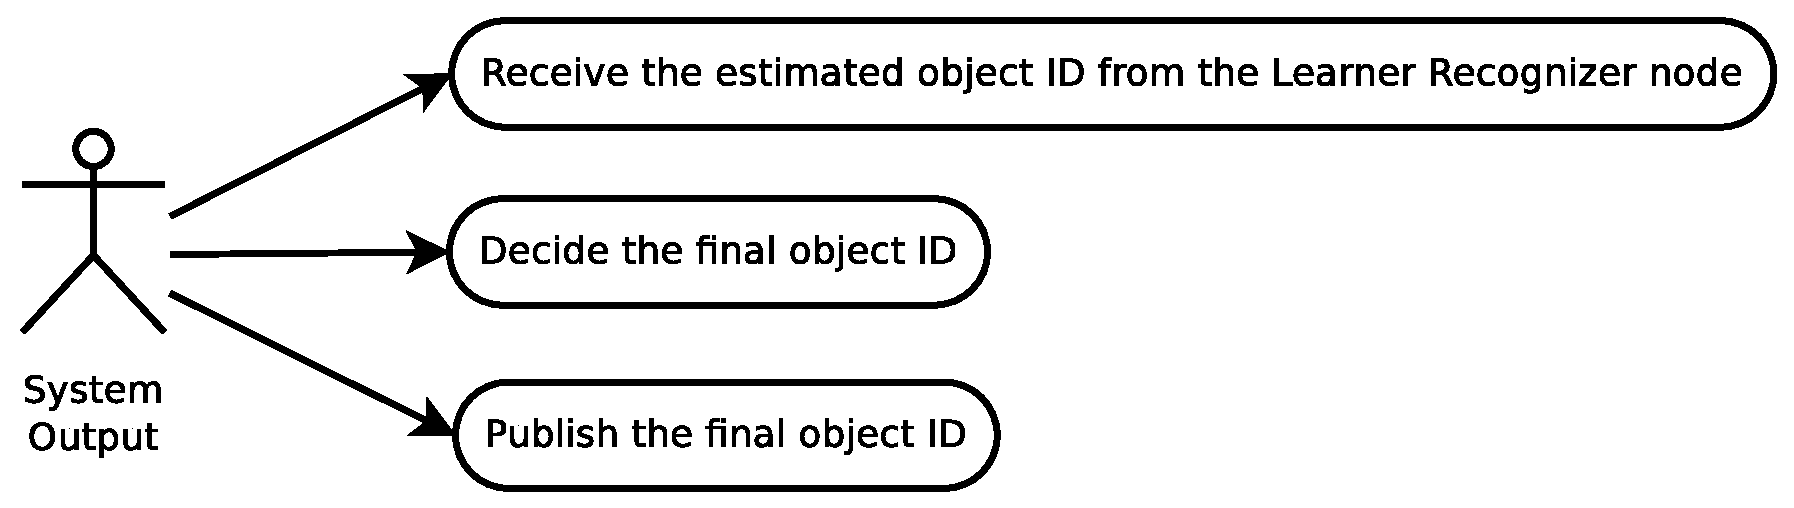
\includegraphics[scale=0.4]{img/diagrams/uc_system_output.eps}
			\caption[Use case diagram System Output node]{Use Case diagram of the System Output node}
			\label{uc_output}
	\end{figure}
 
\newpage
\subsection{Topics}
\label{topics}

	The topics are the channels that communicate the nodes in the ROS framework. All the nodes in the software are constantly obtaining messages from the input topics and publishing the results of their computation to the output ones. 
	\\

	In this section a relation of all the topics used in the software is presented. 


	\paragraph{Hand location}\mbox{} \\

	The complete path of this node in the code is: /TFG/CONVERTER/hand\_location. The messages published in this node are the custom HandLoc message. It specifies the location of both user's hands in the space. 
	\\

	\paragraph{Event}\mbox{} \\

	This node is filled by the node event\_handler. The message used by this node is the custom message TFG/EventHandler. The full name of this topic is /TFG/EVENTHANDLER/event. 

	\paragraph{Descriptors 2D}\mbox{} \\

		The complete name is /TFG/FE2D/descriptors2D. In this topic the Feature Extractor 2D node publishes the matrix of descriptors extracted from the segmented image. To this topic the Learner Recognizer node is subscribed in order to obtain those descriptors.  \\

	\paragraph{Descriptors 3D}\mbox{} \\

		In this topic the Feature Extractor 3D publishes the descriptors of the segmented point cloud. The Learner Recognizer node is subscribed to it. 
		The complete path to the topic is /TFG/FE3D/descriptors3D.\\


	\paragraph{Segmented image}\mbox{} \\

		The path  is /TFG/ROI2D/segmented\_image. In this topic the  ROI Segmenter 2D node publishes its output, the image with the region of interest. To this topic the Feature Extractor 2D is subscribed. \\


	\paragraph{Image with keypoints}\mbox{} \\

		The topic's name is /TFG/ROI2D/segmented\_image\_with\_keypoints. This topic is filled with images showing the segmented 2D ROI with the keypoints drawn on it. The node that publishes this data is FeatureExtractor2D. The topic is intended for visualization and troubleshooting purposes. \\

	\paragraph{Segmented coordinates}\mbox{} \\

		This topic is used to publish the information of the ROI location transformed to pixels. The topic is filled by the ROI Segmenter 3D node and the ROI Segmenter 2D node is subscribed to it. 
			\\
		The complete path of the topic is /TFG/ROI3D/segmented\_coordinates\_px. 

	\paragraph{Segmented pc}\mbox{} \\

		The present topic contains the messages with the segmented point clouds. It is filled by the ROI Segmenter 3D node as well and the Feature Extractor 3D node is subscribed to it. It is also possible to visualize using rviz or other point cloud visualization software the segmented point cloud. 
		\\

		The complete path to the topic is /TTFG/ROI3D/segmented\_pc.


	\paragraph{Object id}\mbox{} \\

		The name of the topic is /TFG/object\_id. This is the output of the system. The topic is filled by a custom message that contains information about the identification number of the recognized object and the grade of certainty in the recognition.\\

		Currently, the topic is only used in order to create a small feedback environment with the user. As part of the future work, another node could be developed to complete a natural interface with the user. This node would allow to give the learned object a name by talking to the software and in turn the code would output the recognized object as audio. For more information please read section \ref{conclusions}.

\newpage
\section{Software messages}
\label{software_messages}

% \newpage
% \subsection{Usage}
\label{usage}

In the present section the compilation and installation instructions of the software are presented as well as the usage instructions. 

\subsubsection{Operating System}
This project uses the ROS framework to compile and run. Since ROS is only available for Linux OS, this type of operating system should be installed in the computer used to run the code. 


\subsubsection{Software needed}
In order to use the software developed in this bachelor's thesis, the following packages are needed. 
\subsubsection{ROS}
The Robotic Operating System is used within the software as the means of communication between the different nodes. Also, different ROS packages are used to provide the input information to the system. Hence, it is needed to install it. 
\\

The code has been tested with the Groovy or Indigo ROS distributions. For installation instructions the webpage http://ros.org provide numerous tutorials. 
\\

Between those distributions there is another one which is called Hydro. For this particular one the code has not been tested but since there are no major changes between Hydro and Indigo, the code used for this latter should compile without problems. 


\subsubsection{ROS package: openni\_camera / freenect\_camera}
These packages are the drivers of the kinect. They should be installed via command-line, which is the recommended, or downloading and compiling the source code. 
\\

In order to install these packages using the terminal, please introduce the following commands: 
\\

sudo apt-get install ros-<distro>-openni\_camera
\\

sudo apt-get install ros-<distro>-freenect\_camera
\\

Replace the <distro> word by the distribution currently installed on your computer, Groovy or Indigo, in lower case. 



\subsubsection{ROS package: openni\_launch / freenect\_launch}
These package needs to be launched in parallel with the code provided in this bachelor's thesis. As the previous ones, they can be downloaded using the terminal or compiling the source code. 
\\

In oder to install them using the command-line please enter the following on it: 
\\

sudo apt-get install ros-<distro>-openni\_launch
\\

sudo apt-get install ros-<distro>-freenect\_launch
\\

This commands install the ROS package in the default directory in which the ROS libraries are stored, usually /opt/ros/<distro>. 



\subsubsection{ROS package: pi\_tracker}
The pi\_tracker package is needed in order to retrieve the position of the user's skeleton. Unfortunately it is not available for command-line installing. This means that the code must be downloaded and compiled in order to be used. 
\\

To do so, the source code must be downloaded into the ROS workspace already created. The source code might be found on the web-page: http://github.com/pi\_tracker. 
\\

For further details on how to download and install ROS packages using the source code please read the following section. 

\subsection{ROS packages source code compilation}
The first thing needed is the ROS workspace. Depending on the ROS distribution, this workspace might be a catkin workspace or a rosbuild workspace. 
\\

Catkin and rosbuild are two methods implemented by ROS to organize the code and to compile it. Both use CMAKE below to compile the code, with specific arguments for different compilation options. 
\\

\subsubsection{Catkin workspace}
The first thing needed is to create a folder for the workspace and a src folder within the first one. This can be done through the interface or using the following command in a terminal: 
\\

mkdir -p <path-to-workspace>/<name-of-workspace>/src\\

Then, insert the following command or open a terminal inside the src folder: \\

cd <path-to-workspace>/<name-of-workspace>/src\\

Finally, in order to initiate the catkin workspace, type: \\

catkin\_init\_workspace\\

This creates an empty workspace. The different packages must be located inside the src folder. \\

In order to build the workspace, move to the upper folder of your workspace and insert the following command: \\

catkin\_make\\

This compiles all the packages within the catkin workspace. In order to use the packages inside this folder, it is necessary to source the setup bash files inside the devel folder. This overlays the workspace on top of your ROS environment. Enter the following command: \\

source <path-to-workspace>/<name-of-workspace>/devel/setup.bash\\




\subsubsection{Rosbuild workspace}
First, introduce the following command in order to create the workspace folder: \\

mkdir -p <path-to-workspace>/<name-of-workspace> \\

Then, in order to create the workspace the rosws command is needed, which is not installed by default. It can be downloaded using the Ubuntu package manager introducing the following in a terminal: \\

sudo apt-get install python-rosinstall\\

Now it is possible to create the workspace using: \\

rosws init <path-to-workspace>/<name-of-workspace> /opt/ros/<ROS-distro>\\

In a rosbuild workspace the packages are located within the sandbox folder. To create it and set it insert the following: \\

mkdir <path-to-workspace>/<name-of-workspace>/sandbox\\

rosws set  <path-to-workspace>/<name-of-workspace>/sandbox\\

Whenever the entries in the workspace suffer changes, it is necessary to re-source the setup file inside the workspace to make sure the updated ROS\_PACKAGE\_PATH is used. In order to source the workspace introduce this line in a terminal: \\

source <path-to-workspace>/<name-of-workspace>/setup.bash\\




\subsection{OCULAR compilation}
The source code might be found in the repository : http://github.com/irenesanznieto/ocular. There are two branches within that code, one for the Groovy and the other for the Indigo distributions. 
\\




\subsection{Launch files}

\subsection{Run the code}


% %\addcontentsline{toc}{chapter}{Hardware}
\section{Hardware}



 
%%%%%%% INTRODUCTION %%%%%%
%%\addcontentsline{toc}{section}{Introduction}
%\section{Introduction}
The advance in the computer vision discipline is greatly linked with the development in the hardware. The main components of a computer vision system are the following: 

\begin{itemize}
	\item{Power Supply: } Device needed by the other components in order to work. 
	\item{Acquisition device: } Device that captures the world and represents it as an array of data. That data can be two or three dimensional. 
	\item{Processing unit:} Receives the information from the acquisition device and processes it. It is usually programmable. Nowadays the most used processing units are PCs. 
	\item{I/O unit: } Serves as a bridge between the acquisition device and the processing unit if needed. 

\end{itemize}

In this chapter the state of the art of the different acquisition devices is going to be presented. 

%%%%%% ACQUISITION DEVICES %%%%%%
%\addcontentsline{toc}{section}{Acquisition devices}
\subsection{Acquisition devices}
There are different acquisition devices being used in the computer vision field. They are usually classified depending on the output data they provide: 

\begin{itemize}
	\item{Cameras:}	The output data is two-dimensional. 
	\item{RGB-D sensors:} The output data is three-dimensional. 
\end{itemize}

The usage of one or another acquisition device depends on the application. The RGB-D sensors provide a higher number of information than the cameras. They reduce the ambiguities produced by the cameras when projecting the three-dimensional world into to dimensions. But also the RGB-D sensors output a higher amount of data. 
That is why, using three-dimensional information as the input of a software requires a higher-capacity processing unit than using two-dimensional data.



%%%%%% CAMERAS %%%%%%
%%\addcontentsline{toc}{section}{Cameras}
\subsection{Cameras}
\label{cameras}



%%%%%% RGB-D SENSORS %%%%%%
%\addcontentsline{toc}{section}{RGB-D Sensors or Natural Interaction Devices}
\subsection{RGB-D Sensors or Natural Interaction Devices}
\label{rgb-d}
%\addcontentsline{toc}{subsection}{History}
\subsubsection{History}

Computer vision is a field that needs specific hardware to retrieve a description of the world. This description has been done for a number of years in two dimensions. But this changed when the first version of an affordable RGB-D sensor appeared in 2010: the Kinect. This project uses a Kinect RGB-D sensor as the input of the system.
\\

This sensor was designed to be used in games, but developers soon realized the huge potential of the hardware for Computer Vision.  
Now, instead of a two-dimensional information as an input it was possible to have three-dimensional information. 
\\

The Microsoft corporation released the SDK (Software Development Kit) on June, 2011 \cite{kinectSDK}.
\\

But one year before, PrimeSense released their open source drivers and motion tracking middleware called NITE\cite{NITE}. 
PrimeSense is a company that manufactures RGB-D sensors and, in fact, the Kinect is based on their depth sensing reference. Hence, the software released by PrimeSense worked with the Kinect as well. 

From that time on, the OpenSource software related with the kinect has increased as well as the different models of RGB-D sensors available in the market.
In November 2010 OpenNI was created. Openni is an open-source software framework that can read the data from RGB-D sensors \cite{openni}.  

%\addcontentsline{toc}{subsection}{How does the Kinect work?}
\subsubsection{RGB-D sensors in this project}






%%% SYSTEM DESCRIPTION
%\addcontentsline{toc}{part}{System Description}
\part{System Description}
\label{system_description}

%\addcontentsline{toc}{part}{Introduction}
\part{Introduction}


%	
\section{Motivation}

Technology has evolved enormously in the past years. 
% In particular, robotics has changed and moved from controlled spaces such as factories to human inhabited spaces. 
% In section \ref{context} the reasons behind this shift in the robot's location and function were presented. 
% It was also estated that the importance of the perception systems augmented with the inclusion of robots in human-inhabited areas. 
% % This fact increases the importance of the perception systems being integrated. 
% The correct recognition of objects, persons, areas and situations is key for assistive and social tasks. 
Nowadays most of the robots being developed are only able to recognize a small part of their environment. 
% Most computer vision systems are currently used to navigate between points or to locate certain objects and grasp them. 
The decision algorithm of the robots is normally based on the instructions received from the user. 
Those commands are usually given by voice or inputting the desired task on a certain User Interface (UI).
\\

% For the robots to act as aiding personnel to take care of elder or sick people, the evolution of this decision algorithm is crucial. 
The algorithm decision of the robots must be upgraded if they are to perform tasks in a human inhabited area. %act as aiding personnel to take care of elder or sick people. 
They must be able to respond to commands, but also be aware of their environment and respond autonomously to it. 
% As an example, robots must be able to recognize the danger involved in certain objects or situations. 
% Also, they should perceive the environment and the interactions between humans to discern if, for example, they are arguing or if the conversation is not a beneficial one for the patient. 
% This latter example may be seen in the case of an anorexic person who is talking about food and weight with another person. 
% Then, the robot may intervene changing the subject subtly or trying to end the conversation. 
When this change has occurred, the robots may successfully perform the assistive tasks now reserved only to humans. 
But there is still a long way to research, mainly around the perception of the environment. 
The investment needed for its development is now being held due to the recession that appeared in the late 2000s decade, whose effects are nowadays still present. 
Nevertheless, this lack of funding might be mitigated using research, open data and open-source code. 
\\

I strongly believe in the ideals presented by the Open Source Initiative. 
This project is intended to be an open source code that can be a building block for other researchers that work on robot perception.
There are various scientists that have already studied the importance of the objects around the human in the action recognition. 
For example, in \cite{Delaitre}, a study of the human-object interaction in still images was performed in order to relate those objects to actions. 
	This relation between object and action may also be seen in \cite{Fathi}, in which wearable cameras are used to retrieve the input. 
	The objects being hand-held are recognized and the action associated to them is learned. 
	In this thesis I present a system that allows to easily learn and recognize hand-held objects in real time. 
	It is intended to be the previous step to the association between the object and the action. 



% The economic situation described above forced many experienced professionals to trying their luck creating start-ups. Many of the ideas of those enterprises are having nowadays a huge impact on the society. 
% \\

% One of these open-source projects that appeared was the low-cost 3D printers. These machines have changed the manner of investigating many fields, since they allow to design different pieces easily and have a 3D reproduction in a few hours. 
% \\

% Initially, they were used in investigation and more specifically in robotics, but now they are used in many different fields. Among those fields, there are medicine, construction or even food making. 
% \\

% In medicine, they have been a revolution since they allow to create customized and precise pieces in very few time. They have been used for prosthesis and implants for persons of various ages, even for babies. In the prosthesis fields in particular, the 3D printing technology is being a complete revolution. Before, the prosthesis were very expensive and permitted only fixed movements and combinations. The adaptations to each individual were made in the final product itself, trying to make it as comfortable as possible for the wearer. Nowadays, the prosthesis are customized for each patient, reducing the inconveniences and increasing their usability. Also, they can be easily and cheaply adapted for children as an example, who are still experimenting many changes in their bodies. They are much cheaper than they were before, and everyone with a 3D printer may construct one. 
% In order to 3D print a piece a file with its description is needed. There are many web-pages that store open-source designs that ranges from decoration models to complex prosthesis. This fact is decisive because there is not needed a huge amount of knowledge or money to improve the life quality of a person using these technologies. 
% \\

% There are numerous open-source projects and developers that put in common their knowledge to improve the technology being used. I have used many of them in the previous years, to learn about 3D printing, robotics or programming among other fields. 
% \\

% It is a fact that acquiring knowledge would be much difficult if the Open Source initiative has not been invented. This impulsed me towards developing something useful and that could be used by other people. The idea of creating a software that could be used in robotics investigation but also help people at the same time. 
% \\[0.5cm]

% Many of the projects are aimed at aiding physically impaired people, creating sternal skeletons and robotic arms that could aid them. But a personal fact led me to realize that visually impaired people were not having as much attention. The applications developed for them are still rough to use and also it is difficult for a grown person to develop his remaining senses to supply the information lost. 
% \\

% Besides, in the robotic field new lines of investigation have appeared. The social robots are now a reality and in the near future we will interact with them everyday. In order to understand the human behavior, the recognition of the objects being handled by them is crucial. 
% \\[0.5cm]


% Computer vision has experience an important improvement in the last years through the upgrade of the hardware and software that compose it. The hardware such as acquisition elements (cameras, depth sensors, etc) and computing elements (PCs or other programmable devices) have experienced a rapid advance in the past years. It allowed to process more data that is now obtained more accurately and with less noise. This increase in the computing power of the equipment created a possibility of introducing more complex libraries and frameworks and even operating systems. 
% \\

% Now, the technology is available to solve the problems presented, the aid of visually impaired people and the introduction of new information in the social robotics field. This is how the idea behind this thesis appeared: the creation of a modular software that implements an in-hand object recognition algorithm. 
 
%	%\addcontentsline{toc}{chapter}{Socio-economical context}
\section{Socio-economical context}

%Socio-economic - relating to both social and economic factors (social groups and the class system for example)
%Context - The circumstances/environment/events surrounding a specific thing. 



%	%\addcontentsline{toc}{chapter}{Future applications}
\chapter{Future applications}
	% future applications



\chapter{Introduction}
This bachelor's thesis consists on a software that implements an in-hand object learning and recognition using 2D and 3D information. 
\\

The code is Open-Source and it was designed to be running inside a robot. The idea is to create a new stand-alone module that could be included in every robot using ROS and a kinect or other RGB-D sensor. This way, having different modularized functionalities it could be possible to create a customized robot in a few seconds, just importing packages and compiling them. 
\\[1cm]

\chapter{Context and motivation}
In the past fifteen years, there has been a change in the perception of the knowledge and whether it should be restricted using patents or not. Most of the scientific community now supports the open source initiative and this has caused a huge increase on the investigation field. \\



The idea of creating common software, of aiding other investigators to easily replicate the work already done and continue from that point instead of "reinventing the wheel" started in the past century. In 1998 the Open Source Initiative (OSI)\cite{osi} was formed, and its definition is recognized as the standard. According to them, "Open source does not just mean access to the source code. The distribution terms of open-source software must comply with the following criteria: Free Redistribution, Source Code, Derived Works, Integrity of The Author's Source Code, No Discrimination Against Persons or Groups, No Discrimination Against Fields of Endeavor, Distribution of License, License Must Not Be Specific to a Product, License Must Not Restrict Other Software,  License Must Be Technology-Neutral"\cite{osi_def}. 
\\

It is my believe that Open Source is critical in the development of new knowledge and not only in the Software field, but in all the science and technical disciplines. This is how the idea of increasing that common pool of tools with another one that might be useful appeared. 
\\
%\begin{wrapfigure}{r}{0.3\textwidth}
%	\centering
%   
\includegraphics[width=0.25\textwidth]{img/intro/open_source.eps}
%	\caption[Open Source Initiative Logo]{Open Source Initiative Logo}
%\end{wrapfigure}

\begin{figure}[h]
	\begin{center}
    
\includegraphics[scale=0.2]{img/intro/open_source.eps}
	\caption[Open Source Initiative Logo]{Open Source Initiative Logo}
	\end{center}
\end{figure}


It is noticeable the mark that Open Source has throughout the project. From the libraries being used in it to the Robotic Operating System of which this project is but another package. All of them are Open Source. Also, the tutorials, examples and different web-pages with useful comments and aids for those who are learning has been critical in this project's development. Nothing of this could have been possible without the idea of Open Source code. 
\\

%Apart from the want of making useful Open Source code, there remains another motivation unexplained. That is, the specific subject of this project. 
\\

%The bad economic context that exist nowadays has forced the different areas of the society to investigate new technologies that has a lower cost. 
%Nowadays, advances regarding robotics appear everyday, and technologies such as 3D printing are having a tremendous impact in the society. Thanks to this instruments, now it is possible and relatively easy to customize prosthesis and also much affordable than it was before. 
%\\

%Robotics is a field that is experiencing a huge impulse currently. And more specifically, Open Source robotics is growing rapidly. 
%\\

One of the open-source projects that appeared with this new way of thinking was the low-cost 3D printers. These machines have changed the manner of investigating in robots, since they allow to design them easily and have a 3D reproduction in a few hours. 
\\

But they are used not only in robots, but also in medicine and many other fields. In medicine, they have been a revolution since they allow to create customized pieces in very few time. They have been used for prosthesis and implants for persons of various ages, even for babies. 
\\

Before, the prosthesis were very expensive and permitted only fixed movements and combinations. The adaptations to each individual were made in the final product itself, trying to make it as comfortable as possible for the wearer. Nowadays, the prosthesis are customized for each patient, reducing the bothers for them and increasing their usability. Also, they can be easily and cheaply adapted for children as an example, who are still experimenting many changes in their bodies. They are much cheaper than they were before, and everyone with a 3D printer may construct one. 
\\

Of course, in order to 3D print a piece a file with its description is needed. There are many web-pages that store open-source designs that ranges from decoration models to complex prosthesis. This fact is decisive because there is not needed a huge amount of knowledge or money to improve the life quality of a person using these technologies. 
\\

There are numerous open-source projects and developers that put in common their knowledge to improve the technology being used. I have used many of them in the previous years, to learn about 3D printing, robotics or programming among other fields. 
\\

The fact that previously I have developed other projects involving designing and constructing 3D-printed wheeled robots gave me the idea of developing a new package for different robots that allowed to easily obtain new functionalities.One of the most interesting fields that can be used in virtually all types of robots is Computer Vision. 
\\

Computer vision has experience an important improvement in the last years through the upgrade of the hardware and software that compose it. The hardware such as acquisition elements (cameras, depth sensors, etc) and computing elements (PCs or other programmable devices) have experienced a rapid advance in the past years. It allowed to process more data that is now obtained more accurately and with less noise. This increase in the computing power of the equipment created a possibility of introducing more complex libraries and frameworks and even operating systems. 
\\

But Computer Vision is an ample area, why choosing object recognition? The project being developed is intended to be useful, not just a mere hobby. It occurred to me that apart from being useful in the interaction with robots and cognitive robots more particularly, this software could be used with visually impaired people, as an example. Mainly, with people that had a sudden loss of vision and that is not used to detect the objects by its shape, or cannot differentiate them by the contour. 
\\

In summary, the software developed is open-source and is intended as a useful package for visually impaired persons, as well as for its integration within a robotic system. 

\newpage
%\addcontentsline{toc}{part}{Introduction}
\part{Introduction}


%	\input{intro/motivation} 
%	\input{intro/context}
%	\input{intro/uses}	% future applications



\chapter{Introduction}
This bachelor's thesis consists on a software that implements an in-hand object learning and recognition using 2D and 3D information. 
\\

The code is Open-Source and it was designed to be running inside a robot. The idea is to create a new stand-alone module that could be included in every robot using ROS and a kinect or other RGB-D sensor. This way, having different modularized functionalities it could be possible to create a customized robot in a few seconds, just importing packages and compiling them. 
\\[1cm]

\chapter{Context and motivation}
In the past fifteen years, there has been a change in the perception of the knowledge and whether it should be restricted using patents or not. Most of the scientific community now supports the open source initiative and this has caused a huge increase on the investigation field. \\



The idea of creating common software, of aiding other investigators to easily replicate the work already done and continue from that point instead of "reinventing the wheel" started in the past century. In 1998 the Open Source Initiative (OSI)\cite{osi} was formed, and its definition is recognized as the standard. According to them, "Open source does not just mean access to the source code. The distribution terms of open-source software must comply with the following criteria: Free Redistribution, Source Code, Derived Works, Integrity of The Author's Source Code, No Discrimination Against Persons or Groups, No Discrimination Against Fields of Endeavor, Distribution of License, License Must Not Be Specific to a Product, License Must Not Restrict Other Software,  License Must Be Technology-Neutral"\cite{osi_def}. 
\\

It is my believe that Open Source is critical in the development of new knowledge and not only in the Software field, but in all the science and technical disciplines. This is how the idea of increasing that common pool of tools with another one that might be useful appeared. 
\\
%\begin{wrapfigure}{r}{0.3\textwidth}
%	\centering
%   
\includegraphics[width=0.25\textwidth]{img/intro/open_source.eps}
%	\caption[Open Source Initiative Logo]{Open Source Initiative Logo}
%\end{wrapfigure}

\begin{figure}[h]
	\begin{center}
    
\includegraphics[scale=0.2]{img/intro/open_source.eps}
	\caption[Open Source Initiative Logo]{Open Source Initiative Logo}
	\end{center}
\end{figure}


It is noticeable the mark that Open Source has throughout the project. From the libraries being used in it to the Robotic Operating System of which this project is but another package. All of them are Open Source. Also, the tutorials, examples and different web-pages with useful comments and aids for those who are learning has been critical in this project's development. Nothing of this could have been possible without the idea of Open Source code. 
\\

%Apart from the want of making useful Open Source code, there remains another motivation unexplained. That is, the specific subject of this project. 
\\

%The bad economic context that exist nowadays has forced the different areas of the society to investigate new technologies that has a lower cost. 
%Nowadays, advances regarding robotics appear everyday, and technologies such as 3D printing are having a tremendous impact in the society. Thanks to this instruments, now it is possible and relatively easy to customize prosthesis and also much affordable than it was before. 
%\\

%Robotics is a field that is experiencing a huge impulse currently. And more specifically, Open Source robotics is growing rapidly. 
%\\

One of the open-source projects that appeared with this new way of thinking was the low-cost 3D printers. These machines have changed the manner of investigating in robots, since they allow to design them easily and have a 3D reproduction in a few hours. 
\\

But they are used not only in robots, but also in medicine and many other fields. In medicine, they have been a revolution since they allow to create customized pieces in very few time. They have been used for prosthesis and implants for persons of various ages, even for babies. 
\\

Before, the prosthesis were very expensive and permitted only fixed movements and combinations. The adaptations to each individual were made in the final product itself, trying to make it as comfortable as possible for the wearer. Nowadays, the prosthesis are customized for each patient, reducing the bothers for them and increasing their usability. Also, they can be easily and cheaply adapted for children as an example, who are still experimenting many changes in their bodies. They are much cheaper than they were before, and everyone with a 3D printer may construct one. 
\\

Of course, in order to 3D print a piece a file with its description is needed. There are many web-pages that store open-source designs that ranges from decoration models to complex prosthesis. This fact is decisive because there is not needed a huge amount of knowledge or money to improve the life quality of a person using these technologies. 
\\

There are numerous open-source projects and developers that put in common their knowledge to improve the technology being used. I have used many of them in the previous years, to learn about 3D printing, robotics or programming among other fields. 
\\

The fact that previously I have developed other projects involving designing and constructing 3D-printed wheeled robots gave me the idea of developing a new package for different robots that allowed to easily obtain new functionalities.One of the most interesting fields that can be used in virtually all types of robots is Computer Vision. 
\\

Computer vision has experience an important improvement in the last years through the upgrade of the hardware and software that compose it. The hardware such as acquisition elements (cameras, depth sensors, etc) and computing elements (PCs or other programmable devices) have experienced a rapid advance in the past years. It allowed to process more data that is now obtained more accurately and with less noise. This increase in the computing power of the equipment created a possibility of introducing more complex libraries and frameworks and even operating systems. 
\\

But Computer Vision is an ample area, why choosing object recognition? The project being developed is intended to be useful, not just a mere hobby. It occurred to me that apart from being useful in the interaction with robots and cognitive robots more particularly, this software could be used with visually impaired people, as an example. Mainly, with people that had a sudden loss of vision and that is not used to detect the objects by its shape, or cannot differentiate them by the contour. 
\\

In summary, the software developed is open-source and is intended as a useful package for visually impaired persons, as well as for its integration within a robotic system. 

\newpage
\input{intro/intro} 
\newpage
\input{intro/thesis_structure}
 
\newpage
\addcontentsline{toc}{chapter}{Thesis structure}
\chapter*{ Thesis structure}


%\addcontentsline{toc}{chapter}{Hardware}
\section{Hardware}



 
%%%%%%% INTRODUCTION %%%%%%
%%\addcontentsline{toc}{section}{Introduction}
%\section{Introduction}
The advance in the computer vision discipline is greatly linked with the development in the hardware. The main components of a computer vision system are the following: 

\begin{itemize}
	\item{Power Supply: } Device needed by the other components in order to work. 
	\item{Acquisition device: } Device that captures the world and represents it as an array of data. That data can be two or three dimensional. 
	\item{Processing unit:} Receives the information from the acquisition device and processes it. It is usually programmable. Nowadays the most used processing units are PCs. 
	\item{I/O unit: } Serves as a bridge between the acquisition device and the processing unit if needed. 

\end{itemize}

In this chapter the state of the art of the different acquisition devices is going to be presented. 

%%%%%% ACQUISITION DEVICES %%%%%%
%\addcontentsline{toc}{section}{Acquisition devices}
\subsection{Acquisition devices}
There are different acquisition devices being used in the computer vision field. They are usually classified depending on the output data they provide: 

\begin{itemize}
	\item{Cameras:}	The output data is two-dimensional. 
	\item{RGB-D sensors:} The output data is three-dimensional. 
\end{itemize}

The usage of one or another acquisition device depends on the application. The RGB-D sensors provide a higher number of information than the cameras. They reduce the ambiguities produced by the cameras when projecting the three-dimensional world into to dimensions. But also the RGB-D sensors output a higher amount of data. 
That is why, using three-dimensional information as the input of a software requires a higher-capacity processing unit than using two-dimensional data.



%%%%%% CAMERAS %%%%%%
%%\addcontentsline{toc}{section}{Cameras}
\subsection{Cameras}
\label{cameras}



%%%%%% RGB-D SENSORS %%%%%%
%\addcontentsline{toc}{section}{RGB-D Sensors or Natural Interaction Devices}
\subsection{RGB-D Sensors or Natural Interaction Devices}
\label{rgb-d}
%\addcontentsline{toc}{subsection}{History}
\subsubsection{History}

Computer vision is a field that needs specific hardware to retrieve a description of the world. This description has been done for a number of years in two dimensions. But this changed when the first version of an affordable RGB-D sensor appeared in 2010: the Kinect. This project uses a Kinect RGB-D sensor as the input of the system.
\\

This sensor was designed to be used in games, but developers soon realized the huge potential of the hardware for Computer Vision.  
Now, instead of a two-dimensional information as an input it was possible to have three-dimensional information. 
\\

The Microsoft corporation released the SDK (Software Development Kit) on June, 2011 \cite{kinectSDK}.
\\

But one year before, PrimeSense released their open source drivers and motion tracking middleware called NITE\cite{NITE}. 
PrimeSense is a company that manufactures RGB-D sensors and, in fact, the Kinect is based on their depth sensing reference. Hence, the software released by PrimeSense worked with the Kinect as well. 

From that time on, the OpenSource software related with the kinect has increased as well as the different models of RGB-D sensors available in the market.
In November 2010 OpenNI was created. Openni is an open-source software framework that can read the data from RGB-D sensors \cite{openni}.  

%\addcontentsline{toc}{subsection}{How does the Kinect work?}
\subsubsection{RGB-D sensors in this project}


%\addcontentsline{toc}{chapter}{Software}
\section{Software}
\label{software}
 %%%%%%% INTRODUCTION %%%%%%
%%\addcontentsline{toc}{section}{Introduction}
%\section{Introduction}
In this section the software developed in this Bachelor's Thesis is presented and thoroughly explained. 
\\

The code was created as a ROS package. ROS (Robotic Operating System) is an Operating System designed to be implemented in robots. It has libraries to enhance the communication between nodes, the processes management or the threads present in the code among other functionalities. 
Since this code is intended to be running on a robot, the software developed was created as a ROS package. 
\\

In order to manage 2D and 3D information (images and point clouds) two libraries has been used: OpenCV, and PCL. Those two libraries implement basic and state-of-the-art algorithms that allow a easier and more time-efficient management of the data. Further information about these libraries might be found on the sections \ref{opencv} and \ref{pcl} respectively. 
\\

The software was structured in nodes. These nodes have a relatively small functionality and run in parallel. The fact that they run simultaneously improves the efficiency of the code lowering the lag due to time-expensive operations. 
\\

In the following sections, the software structure and tools used are described. 



%\section{Structure}
%\label{structure}

%In this section, the code functionalities of each part or node of the software are explained. The communication between nodes is shown and the overall software flow is thoroughly described. 

The code is structured in nodes. Each node contains a piece of the processing needed in the code. All nodes are related between them using ROS messages to transport the input and output data. 
\\

Computer vision is a field that involves high time-expensive algorithms. In the previous chapter it was explained that it uses 2D and 3D information. That information implies a matrix that has for each point 2 coordinates number (in the case of 2D) or 3 coordinates (in the case of 3D data), apart from the colour of that point, which is described using 3 more integers. \\

As it can be seen the data handled is enormous an the way to reduce the time lag due to those computations is modularizing the computation and executing in parallel those processes. 
\\

The software was designed to be as modular as was possible so that each node performs an action that could be used in other applications. 
As an example, the code could be easily changed to recognize hats or shoes, just changing the initial node that extracts the information of the desired joint. 
\\

In the following paragraphs the nodes' functionalities will be described and the communication between them presented. But first, the overall software work-flow is shown using the flow diagram below. 
\newpage

\subsection{Solution description}

The input of the system is the information coming from the RGB-D sensor. There are two different data that are taken: the 2D information, i.e. the raw image detected by the sensor's camera, and the 3D information, i.e. the raw point cloud. Also, there is another input to the system that shows the position of the different user's joints. This data is provided by a third-party package called pi\_tracker that is explained in the following chapters. 
\\

The software was designed to be running on a robot as was previously explained. This implies that there can not be a GUI (Graphical User Interface) on a screen because the robot being used might not have it. Also, the usability and easiness to learn how to interact with the program was important to allow different people not only investigators to use it. 
\\


\begin{figure}[H]
	\begin{center}
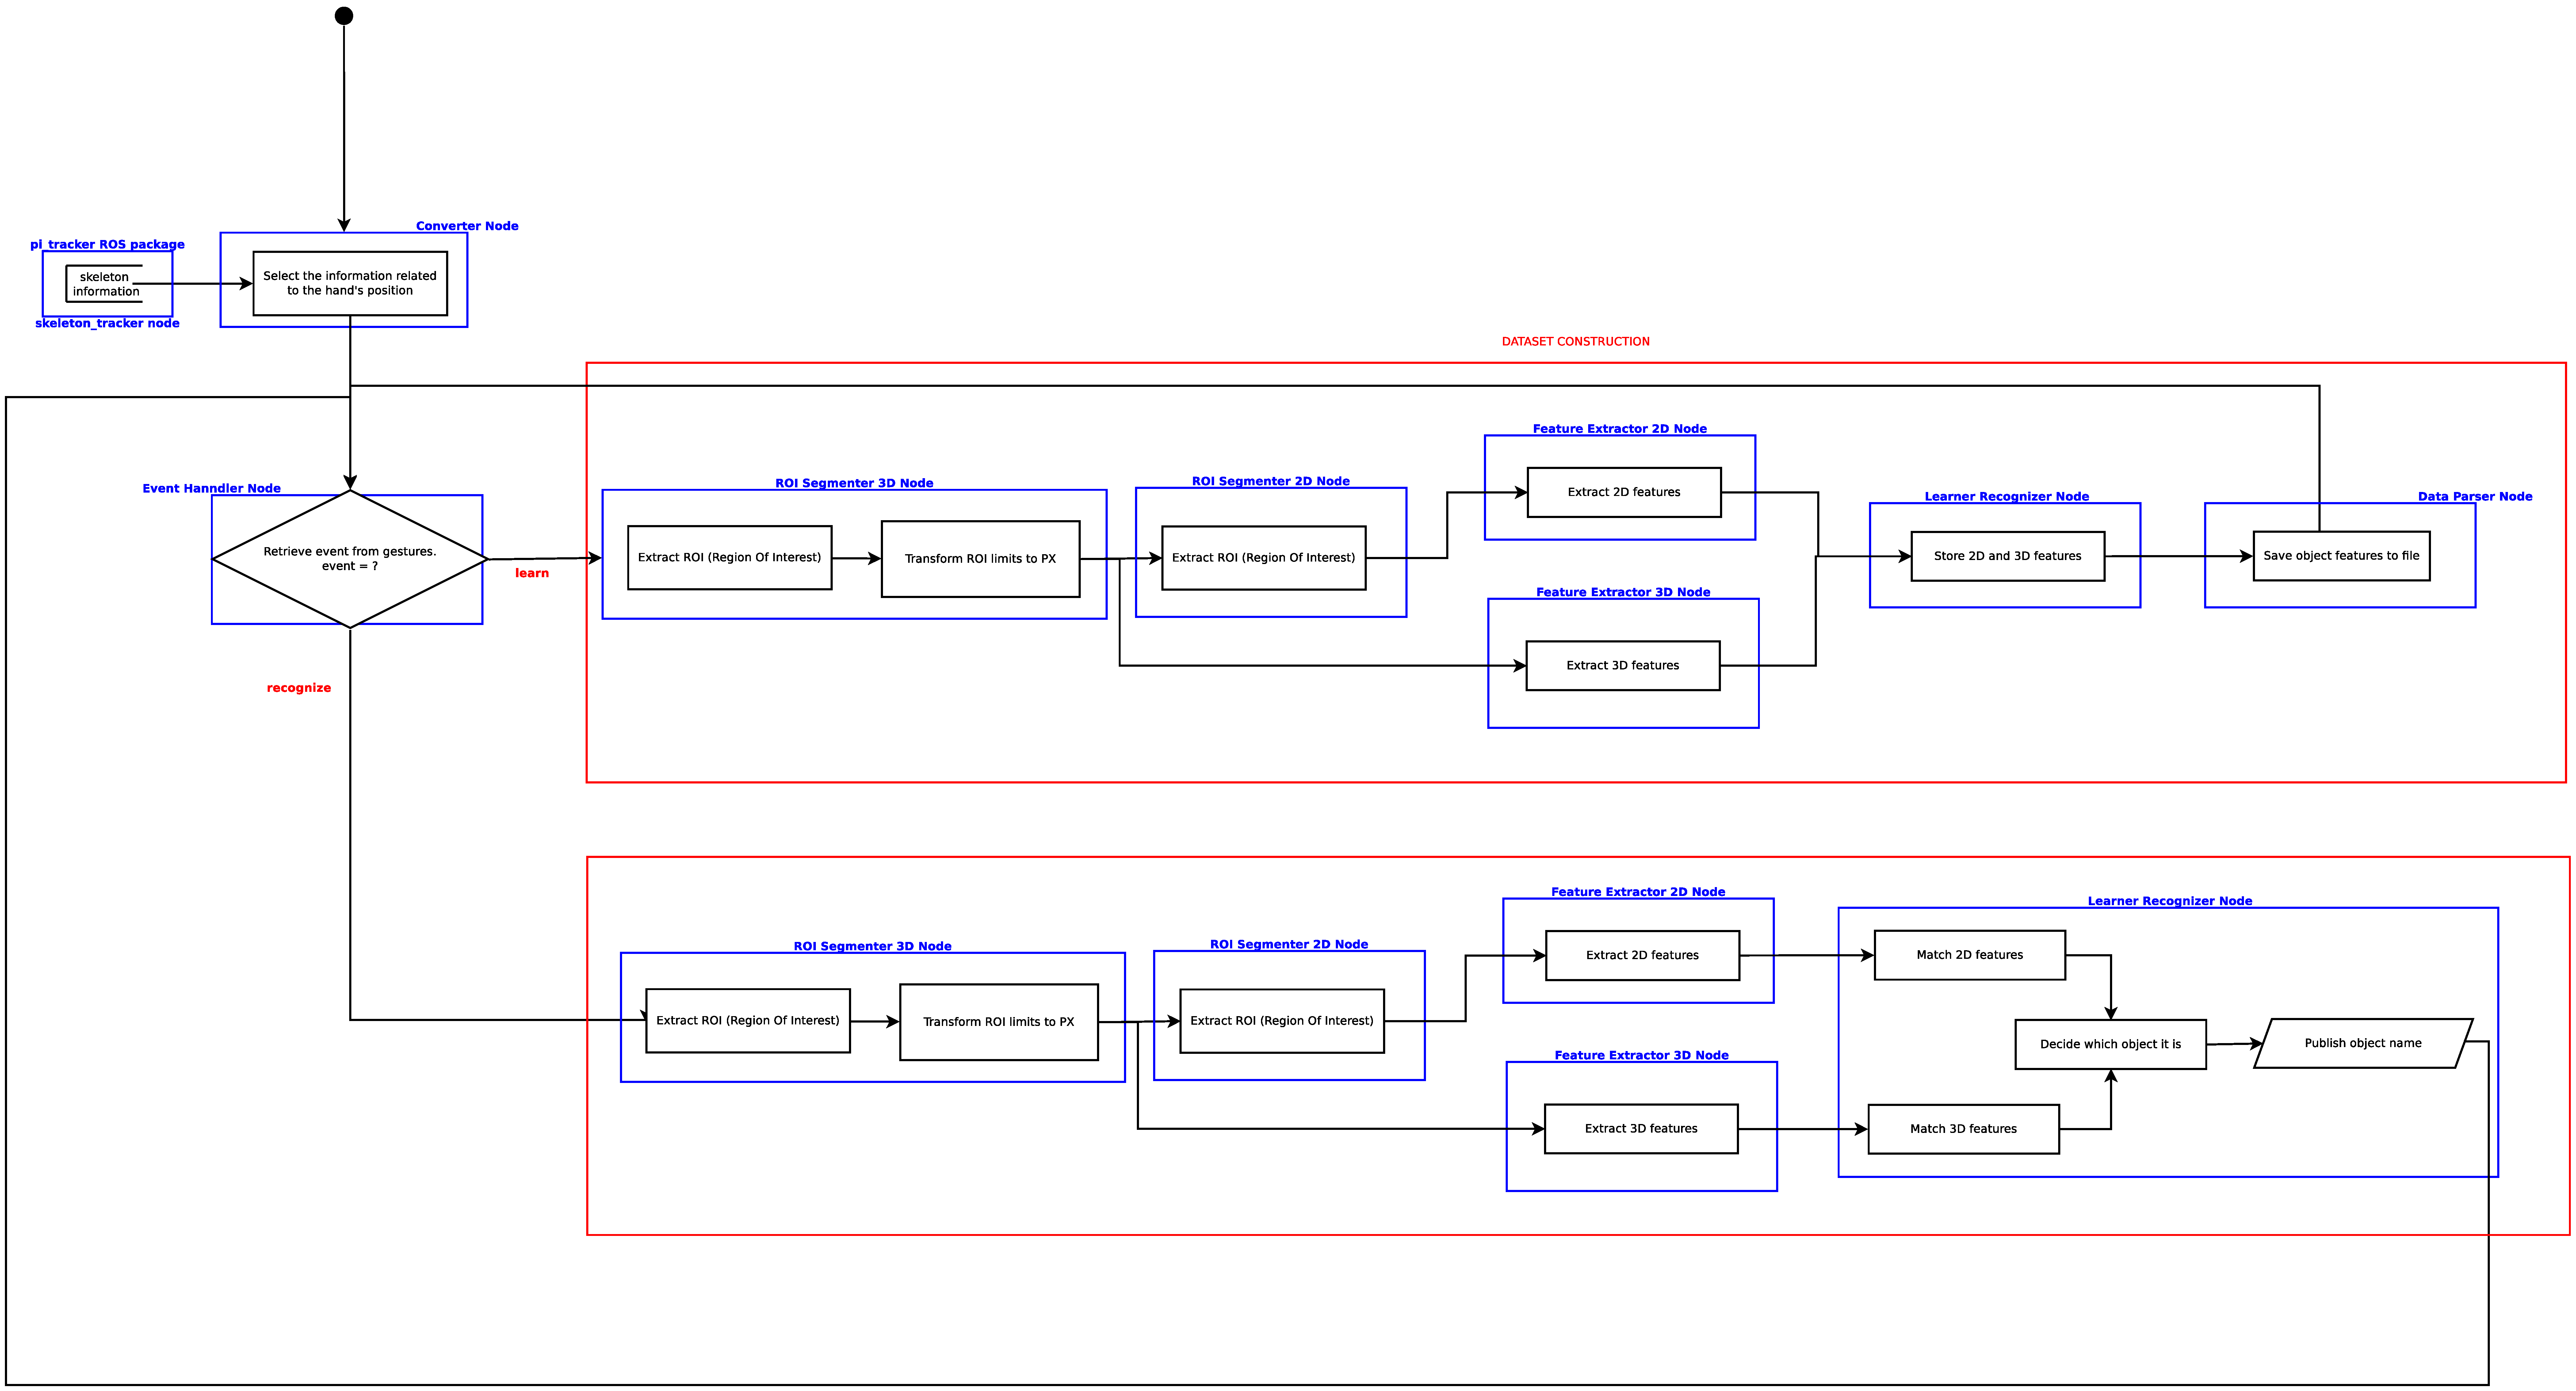
\includegraphics[scale=0.3]{img/diagrams/flowcharts.eps}
	\caption[Software flowchart]{Complete Software flowchart showing the different processing steps between the input and the output}
	\end{center}
\end{figure}


In order to fulfill those requirements a gestural interface was designed. It is developed by a separate node so the processing lags will not affect the recognition of the different gestures. This fact also allows an easy change of the gestures being used. 
\\

The recognition of the location of the hand with respect to the user's body shows how the arm is positioned. If it is stretched towards the sensor, the software enters the dataset construction mode, i.e. the data acquisition and learning mode. If, otherwise, it is located closer to the body, the software starts the object recognition mode. 
\\


The upper part of the diagram shows the data acquisition work-flow. The first step is to extract the ROI (Region of Interest) from the input raw data. This is a crucial step that allows to reduce noticeably the amount of time due to computation reducing the size of the processed information. 
\\

After the extraction, the 2D and 3D features of the segmented data are obtained. The features or descriptors are characteristics that define and represent the data from where they were created. There are different algorithms that perform this task with better or worse repeatability and robustness. All the details about this process is explained in the next chapters. 
\\

That is the end of the data cycle of the learning process. It is iterated over the number of views for each object that is required in order to obtain all the templates necessary per object. 
\\

The recognition mode was triggered when the hand was located near the user's body. This mode can be seen in the lower part of the previous diagram. 
\\

The steps that compose this part of the software are the following: 
First, the input information is converted to the custom message used within the code. Afterwards, as in the previous mode, the Region Of Interest is segmented from both 2D and 3D original information. Then, the descriptors are extracted exactly the same way as in the previous mode. 
\\

The next step is the recognition algorithm. This matches the descriptors from both the image and the point cloud and decides which object of the dataset is more similar to the one that is currently on the user's hand. More details about this algorithm may be found in this section. 
\\

Finally, the object identification number is obtained. This data is the output of the system. 


\newpage
\subsection{Third party libraries that process the input data to the system}
\label{ros_packages}
In this section the ROS packages that are used in our system are presented. 
All of them are used for the initial processing of the data coming from the RGB-D sensor. 
The connection between them and the developed nodes are explained in this section and in section \ref{nodes}.

\subsubsection{ROS package: openni\_camera}
\label{openni_camera}

This package implements the RGB-D sensors drivers.
% It is needed to connect the kinect to the computer. 
% The package is composed of nodes that perform different tasks and publish the results in topics. 
% As an example, a node transforms the raw output information of the kinect into a data array for further processing. 
The package transforms the input raw data coming from the kinect into structured one. 
This information is prepared hence for further processing. 
Figure \ref{diagram_kinect_data} shows the Connectivity graph of this package and its position in the RGB-D sensor data processing chain. 
 
 		\begin{figure}[H]
			\begin{center}
			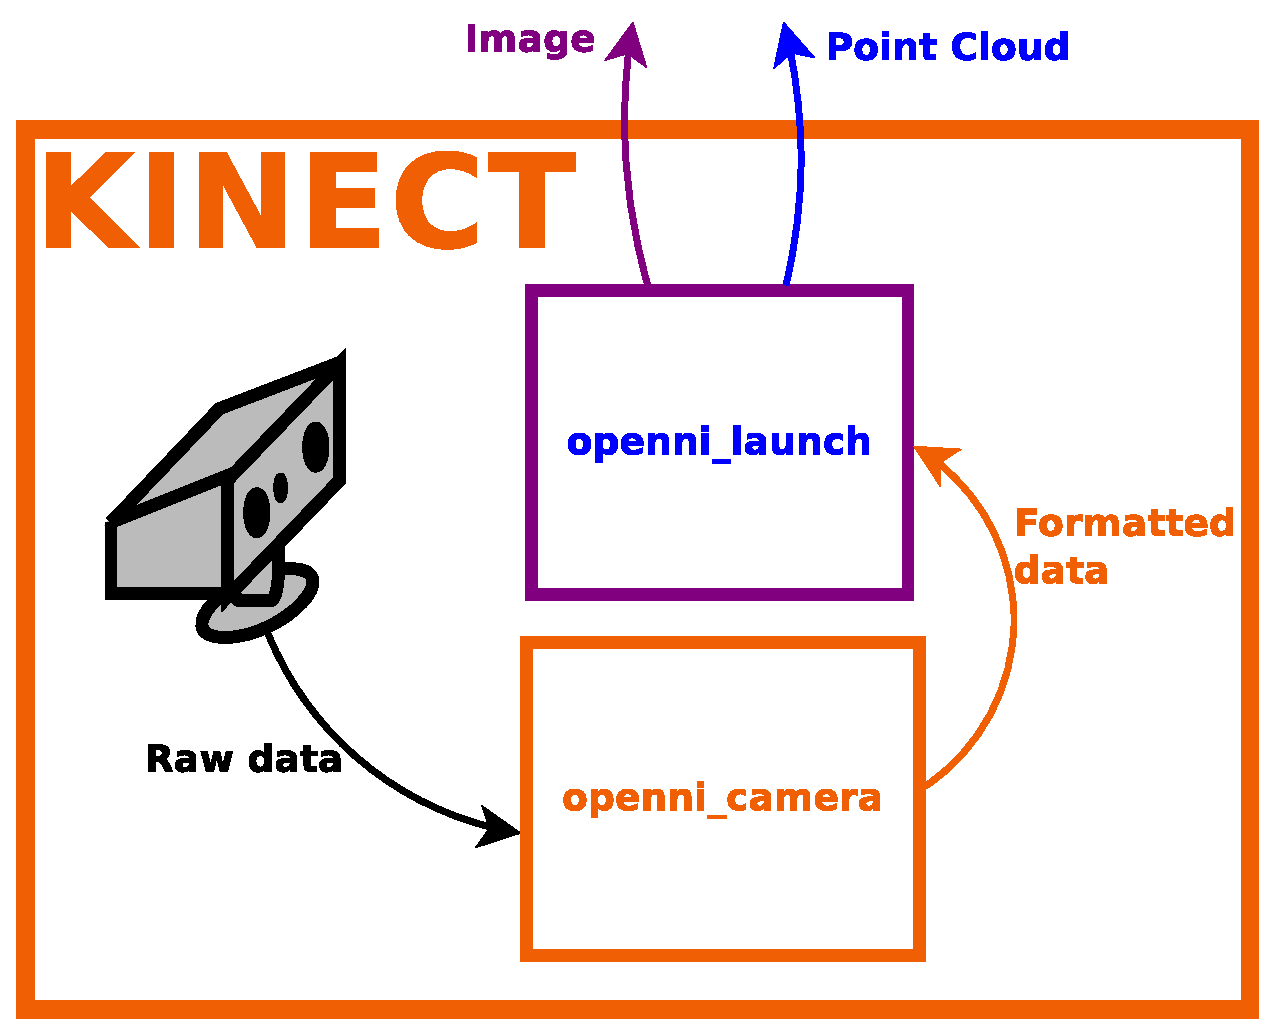
\includegraphics[width=0.5\linewidth]{img/diagrams/kinect_data.eps}
			\caption[Kinect data processing]{Kinect data processing using the openni ROS packages (openni\_camera and openni\_launch).}
			\label{diagram_kinect_data}
			\end{center}
		\end{figure}


\subsubsection{ROS package: openni\_launch}
\label{openni_launch}

This package provides useful transformations taking as input the openni\_camera topics. %and a launch file that executes nodelets with that information. 
It is composed of various nodes that can be executed using a launch file. 
Each node processes the raw input information from the driver into more useful data. 
This data may be a point cloud with color information or a disparity image for example. 
The output of the nodes is published into different topics. 
% The developed nodes described in section \ref{nodes} are subscribed to these topics in order to obtain the input point cloud and image. 
These topics are the input for the nodes that have been developed for this thesis.

\subsubsection{ROS package: pi\_tracker}

This ROS package implements a joint tracker.
It is used within the system to determine the position and orientation of the user's joints. 
This task is performed by the skeleton tracker node.  
Figure \ref{diagram_skeleton} shows the Connectivity graph of this node. 
% In figure \ref{diagram_skeleton} it may be observed that the diagram presented in figure \ref{diagram_kinect_data} is simplified.  

		\begin{figure}[H]
			\begin{center}
			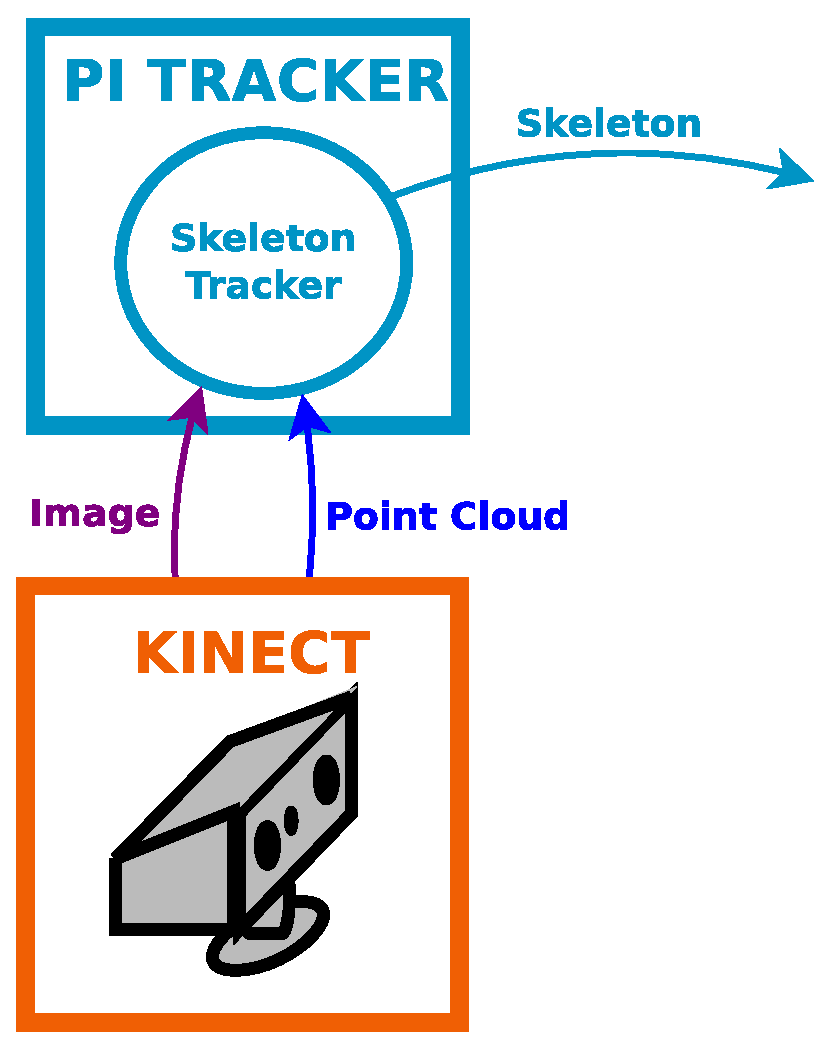
\includegraphics[width=0.3\linewidth]{img/diagrams/node_pi_tracker.eps}
			\caption[Skeleton Tracker I/O]{Connectivity graph of the Skeleton Tracker node.}
			\label{diagram_skeleton}
			\end{center}
		\end{figure}

It can be seen that the node takes as input the output data of the openni\_launch ROS package. 
The node outputs the Skeleton message in which the positions and orientations of the joints are represented. 



%\newpage
%%%%%%% SOFTWARE NODES %%%%%%
%\addcontentsline{toc}{subsection}{Software nodes}
\subsection{Description of the developed nodes}
\label{nodes}


The processing of the system is divided in nodes. 
Figure \ref{nodes_graph} shows the graph of the nodes that have been developed for the project.
% First the ones using the raw input data to the system and afterwards the ones that deliver the output of the system are described.
The circles represent the nodes. %Each circle is a node and the name inside them is the one being used in the software. 
The arrows show the communication between nodes. 
The names next to the nodes' interconnections are the messages interchanged.  % that those processes interchange. 
% The squares with the names serve as separators of the different packages that are being used. 
The square areas define the different ROS packages that have been used.
The square with the tile "OCULAR" separates the nodes developed in this thesis from third-party nodes. 
% All the nodes inside the square with the title "OCULAR" are the ones I developed. 
Sections \ref{converter} to \ref{last_node} present the processing performed by each node. 
\\


		\begin{figure}[H]
			\begin{center}
			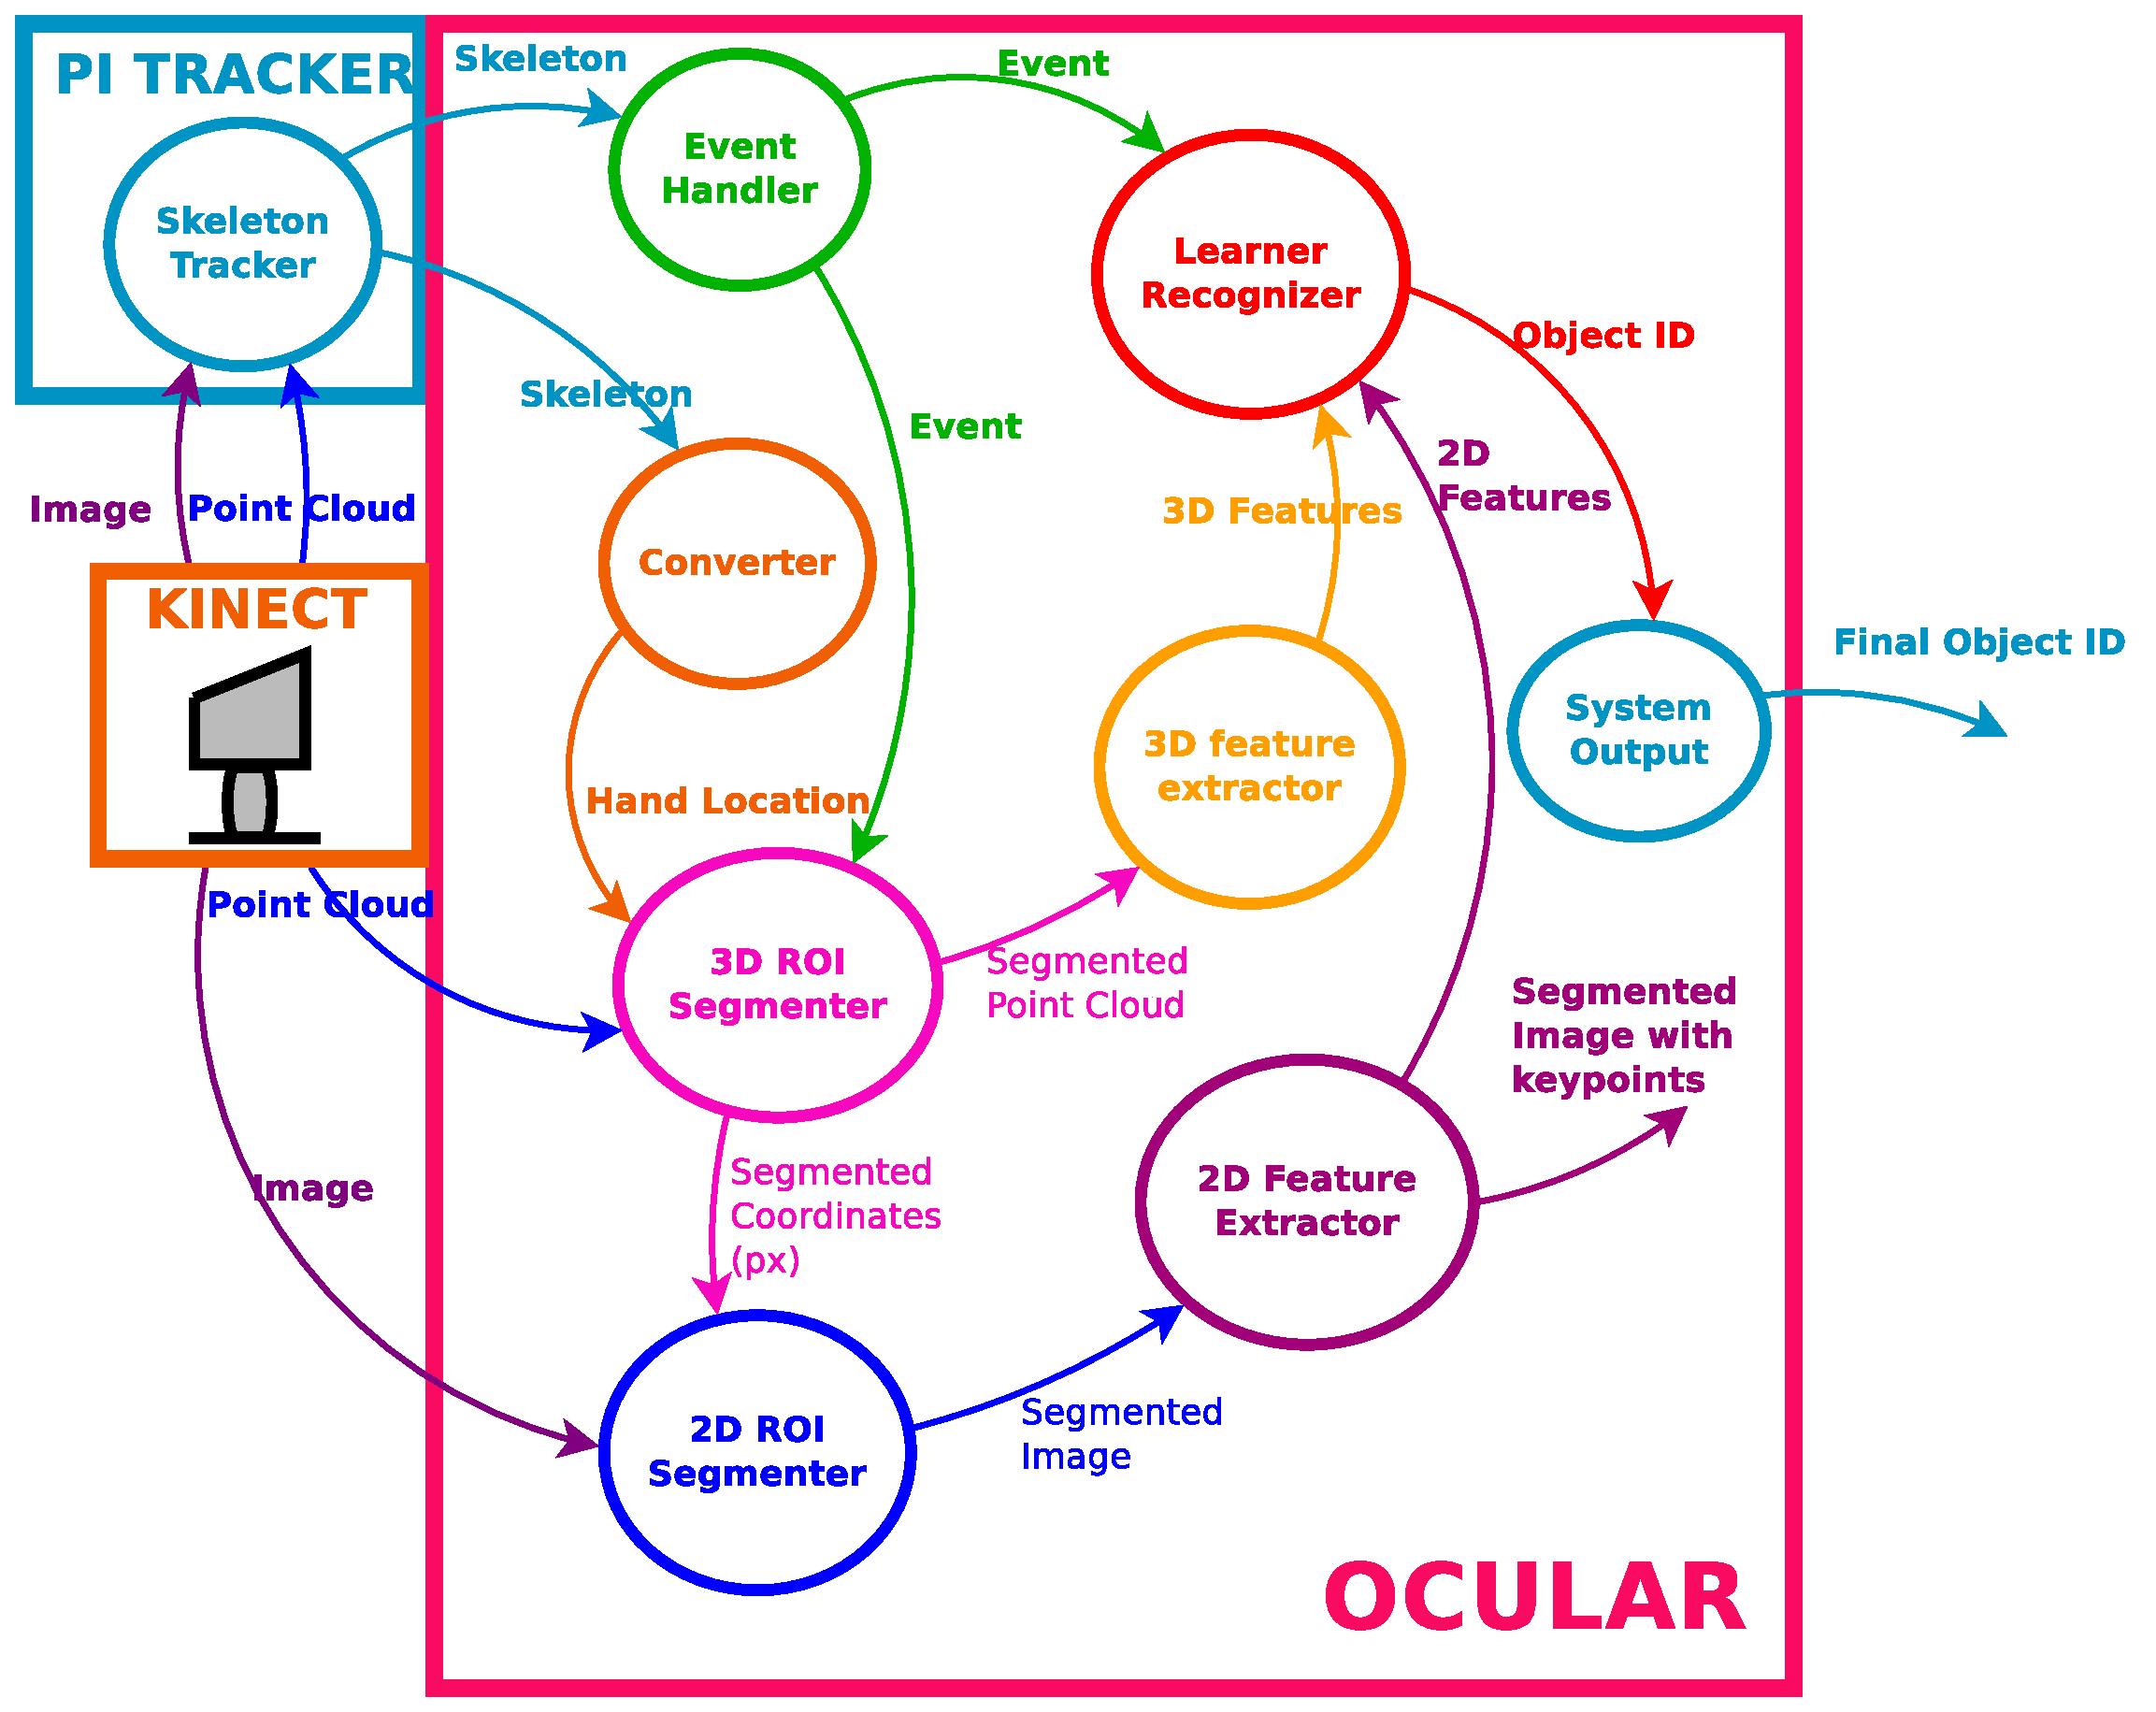
\includegraphics[width=\linewidth]{img/diagrams/nodes.eps}
			\caption[System nodes]{System nodes and their interaction.}
			\label{nodes_graph}

			\end{center}
		\end{figure}

%\newpage



%%\newpage


\subsubsection{Converter node}
		\label{converter}

	This node is the first step of the developed software. 
	It converts the input data containing the skeleton position to a custom message used through the rest of the code. 
	It allows to easily change the package from which the skeleton is obtained without affecting the whole system. 
	The converter node transforms the input data from the pi\_tracker package into the custom message used within the software. 
	It was only implemented a converter for the pi\_tracker package, but it could be easily developed a converter for other packages that retrieve the skeleton position. 
	Figure \ref{node_converter} represents the Connectivity graph of the node. 
	The skeleton message enters the node and the custom message containing the hands location is the output. 

		\begin{figure}[H]
			\begin{center}
			\includegraphics[width=0.5\linewidth]{img/diagrams/node_converter.png}
			\caption[Converter node I/O]{Connectivity graph of the Converter node.}		
			\label{node_converter}
			\end{center}
		\end{figure}

	% The information provided by that third-party code contains the position in the space of each joint of the body. 
	% The converter node takes only both hand's position. 
	The use case diagram of the node can be seen in figure \ref{uc_converter}. 

	\begin{figure}[H]
		\centering
		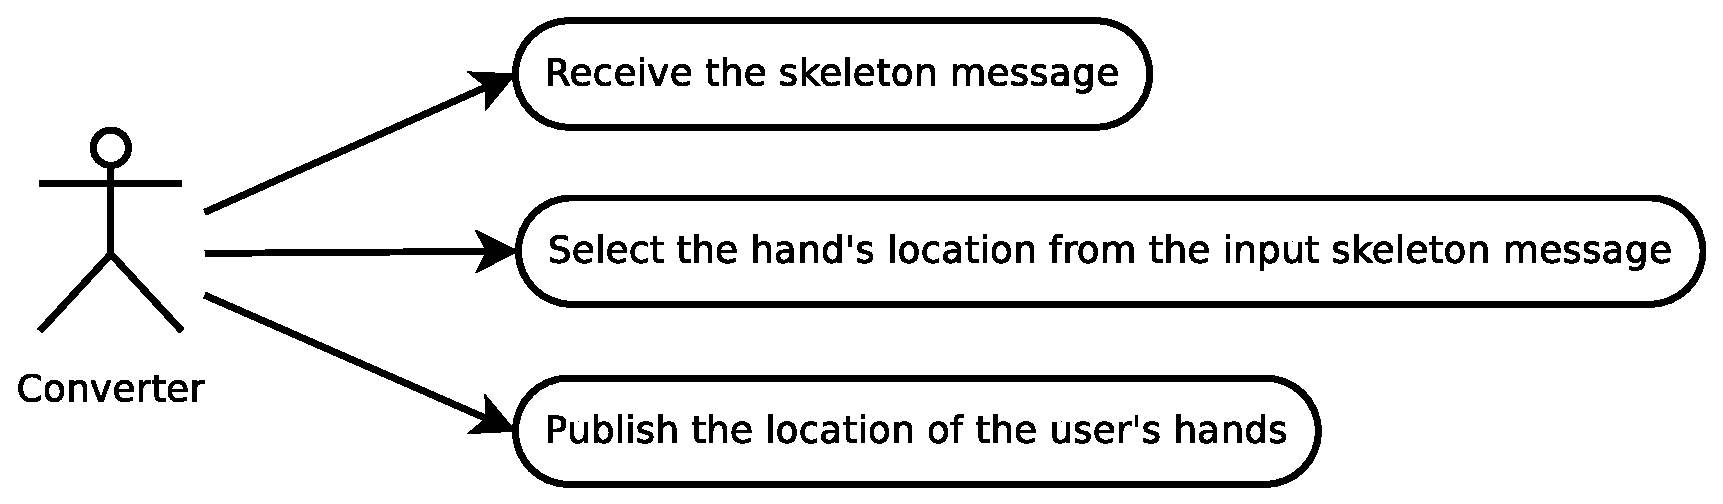
\includegraphics[scale=0.4]{img/diagrams/uc_converter.eps}
		\caption[Use case diagram converter node]{Use Case diagram of the converter node}
		\label{uc_converter}
	\end{figure}

	
	%%\newpage

\subsubsection{3D ROI Segmenter node}
	\label{roi_segmenter_3d}

	Figure  \ref{node_roi3d} presents the Connectivity graph of the node. 
	The input of this node is the raw 3D information from the sensor and the hand's locations from the third-party package pi\_tracker, as well as the hand in which the user is holding the object. 

		\begin{figure}[H]
			\begin{center}
			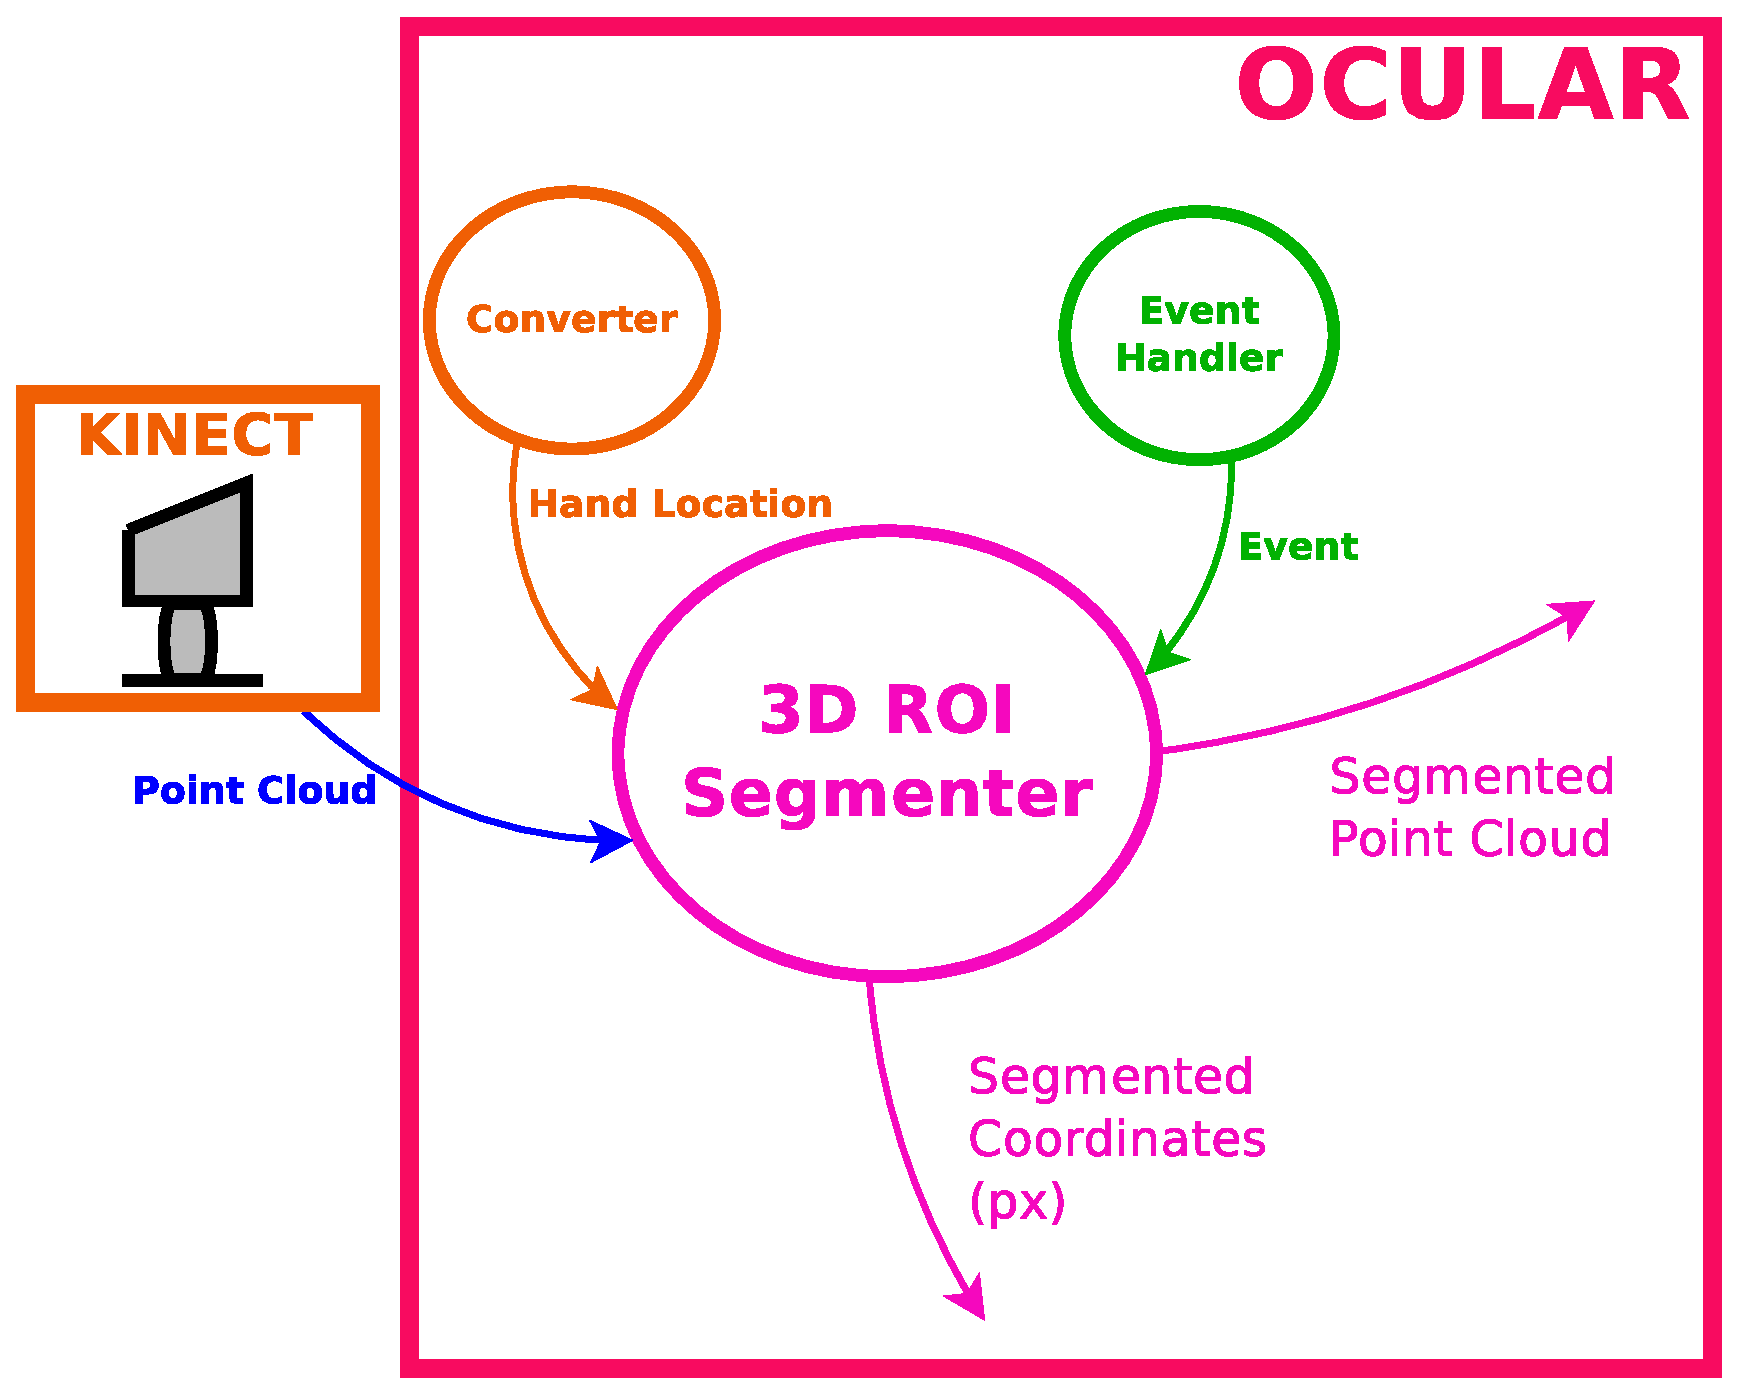
\includegraphics[width=0.5\linewidth]{img/diagrams/node_roi3d.eps}
			\caption[ROI segmenter 3D node I/O]{Connectivity graph of the ROI segmenter 3D node.}		
			\label{node_roi3d}
			\end{center}
		\end{figure}


	The node segments a prism from the original point cloud around the selected hand's center. 
	The prism vertex coordinates are transformed from world coordinates to pixels. 
	This is done to allow the ROI Segmenter 2D to perform the cropping of the input image using those pixel values. 
	That information is the output of the node, together with the segmented point cloud. 
	Figure \ref{uc_roi3d} shows the use case diagram of the node. 

	\begin{figure}[H]
		\centering
	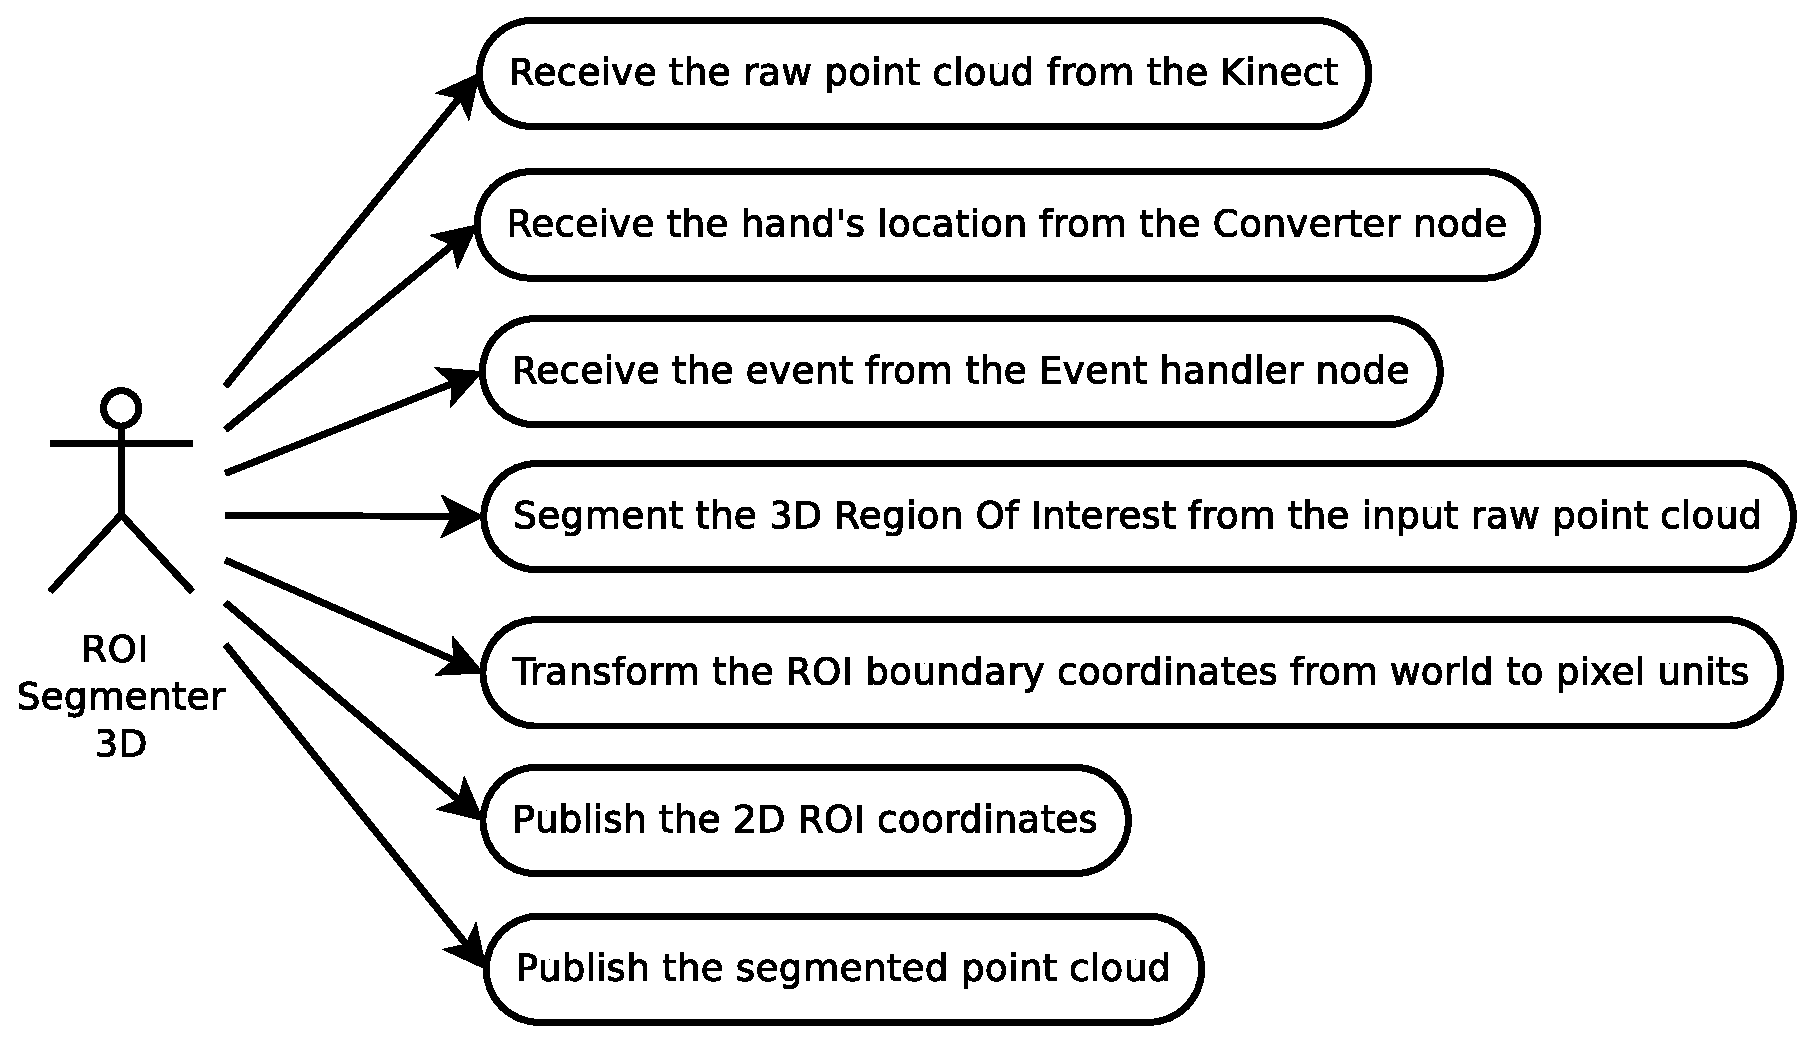
\includegraphics[scale=0.4]{img/diagrams/uc_roi_segmenter_3d.eps}
		\caption[Use case diagram ROI segmenter 3D node]{Use Case diagram of the ROI segmenter 3D node}
		\label{uc_roi3d}	
	\end{figure}
 
%%\newpage

\subsubsection{2D ROI Segmenter node}
	\label{roi_segmenter_2d}
	
	%The present node takes as the input the raw 2D information from the RGB-D sensor and the hand's locations in pixels returned from the ROI segmenter 3D node. 
	Figure \ref{node_roi2d} depicts the Connectivity graph of this node. 
	The raw 2D information and the hand location in pixels are inputs to the ROI Segmenter 2D node. 

		\begin{figure}[H]
			\begin{center}
			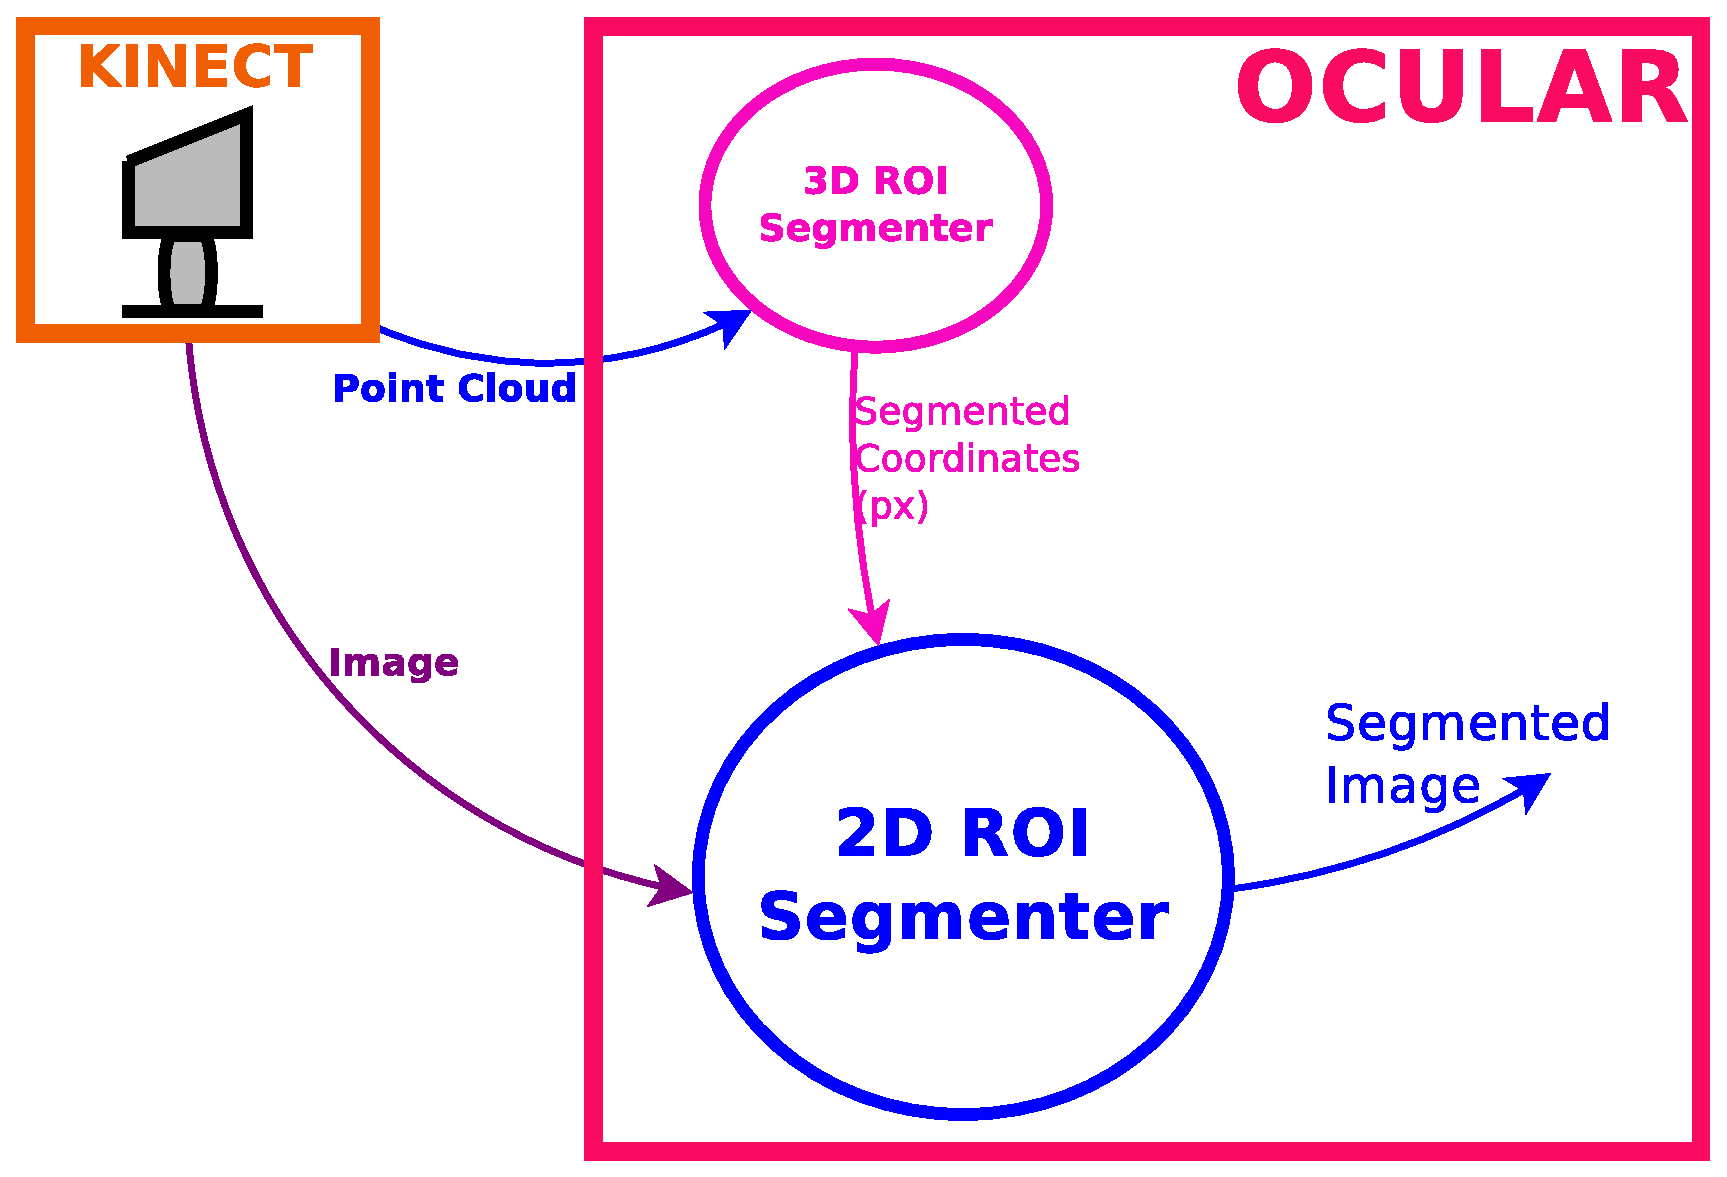
\includegraphics[width=0.5\linewidth]{img/diagrams/node_roi2d.eps}
			\caption[ROI segmenter 2D node I/O]{Connectivity graph of the ROI segmenter 2D node.}		
			\label{node_roi2d}
			\end{center}
		\end{figure}

	The processing performed is the following: First, the ROI (Region Of Interest) is cropped taking a square section around the center of the hand. 
	The size of that figure is fixed for simplicity. 
	This fact does not affect the segmentation since the difference in the scale in negligible in the operating range of the system. 
	The range is determined by the skeleton tracker node and also the low resolution of the RGB-D sensor. 
	The system may be used at a distance between 1.5m and 2.5m. 
	%Since due to the RGB-D sensor's current resolutions the user must remain at a fixed distance from the sensor, the difference in the scale due to the distance is negligible and hence the size can be fixed. 
	\\
	In figure \ref{uc_roi2d} the use case diagram of the node can be observed.
	\begin{figure}[H]
		\centering
			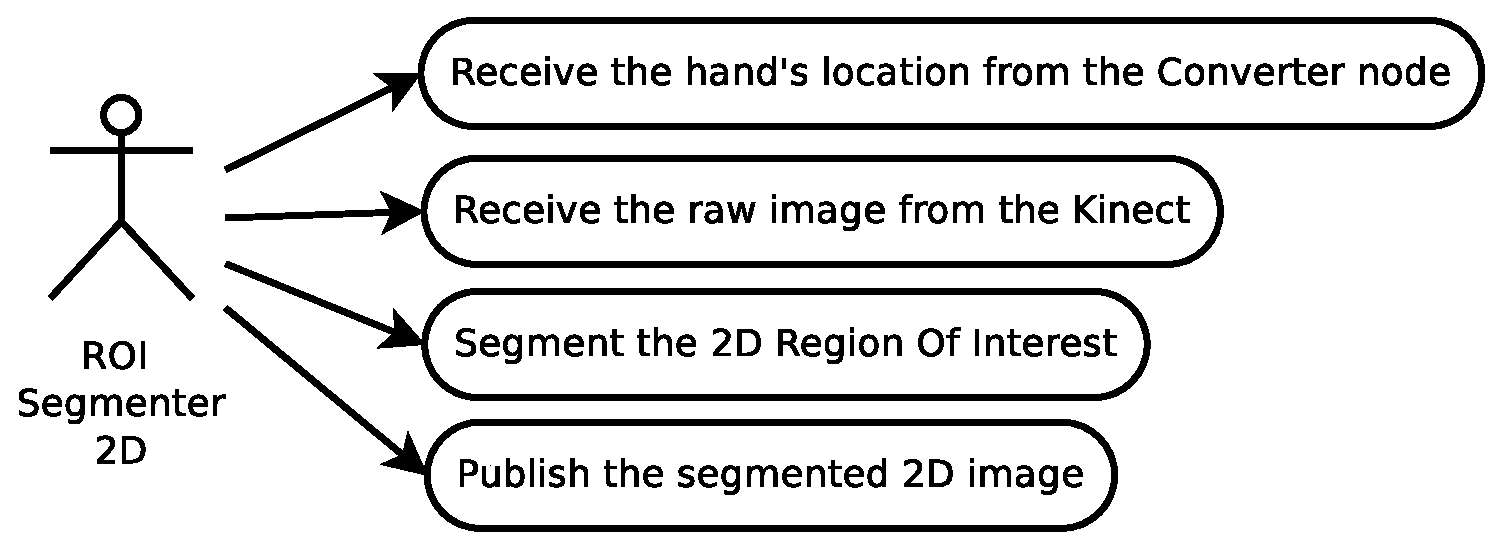
\includegraphics[scale=0.4]{img/diagrams/uc_roi_segmenter_2d.eps}
			\caption[Use case diagram ROI segmenter 2D node]{Use Case diagram of the ROI segmenter 2D node}
		\label{uc_roi2d}
	\end{figure}

%%\newpage

\subsubsection{2D Feature Extractor node}

	This node takes as an input the segmented 2D ROI from the previous nodes and extracts the features. 
	Figure \ref{node_fe2d} shows the Connectivity graph of the node. 

		\begin{figure}[H]
			\begin{center}
			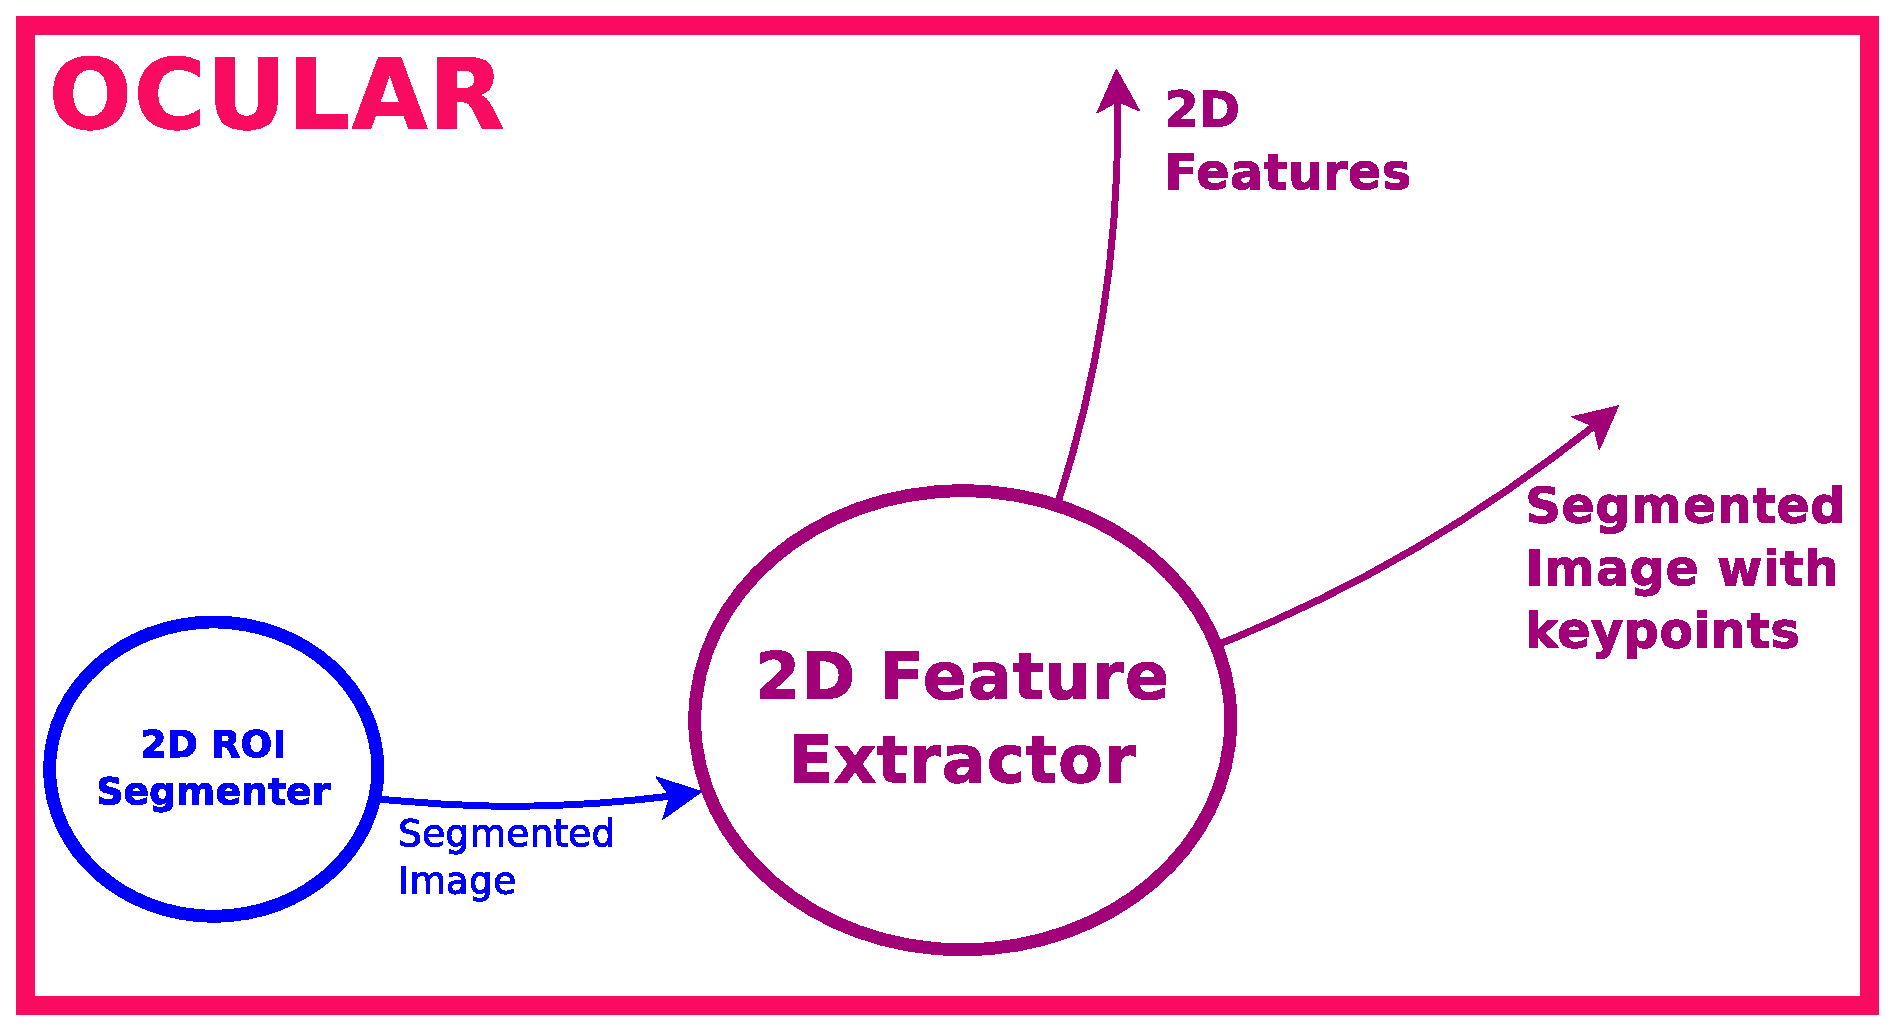
\includegraphics[width=0.5\linewidth]{img/diagrams/node_fe2d.eps}
			\caption[Feature Extractor 2D node I/O]{Connectivity graph of the Feature Extractor 2D node.}		
			\label{node_fe2d}
			\end{center}
		\end{figure}

	There are two output messages of this node, the segmented images with keypoints and the 2D ORB descriptors. 
	The descriptors matrix is the one being used in the rest of the system. 
	The segmented image with the keypoints drawn on it is outputted for debugging and development reasons. 
	\\

	Figure  \ref{uc_fe2d} represents the use case diagram of this node. 
	\begin{figure}[H]
		\centering
			\includegraphics[scale=0.4]{img/diagrams/uc_feature_extractor_2d.eps}
			\caption[Use case diagram Feature Extractor 2D node]{Use Case diagram of the Feature Extractor 2D node}
		\label{uc_fe2d}
	\end{figure}

%%\newpage

\subsubsection{3D Feature Extractor node}

	The input of this node is the segmented point cloud from the ROI Segmenter 3D node (see section \ref{roi_segmenter_3d}. The descriptors are extracted from this information and are published in the output topic. 
	\\
		\begin{figure}[H]
			\begin{center}
			\includegraphics[width=0.5\linewidth]{img/diagrams/node_fe3d.eps}
			\caption[Feature Extractor 3D node I/O]{Connectivity graph of the Feature Extractor 3D node.}		
			\label{node_fe3d}
			\end{center}
		\end{figure}

	Figure \ref{uc_fe3d} shows the use case diagram of the node. 

	\begin{figure}[H]
		\centering
			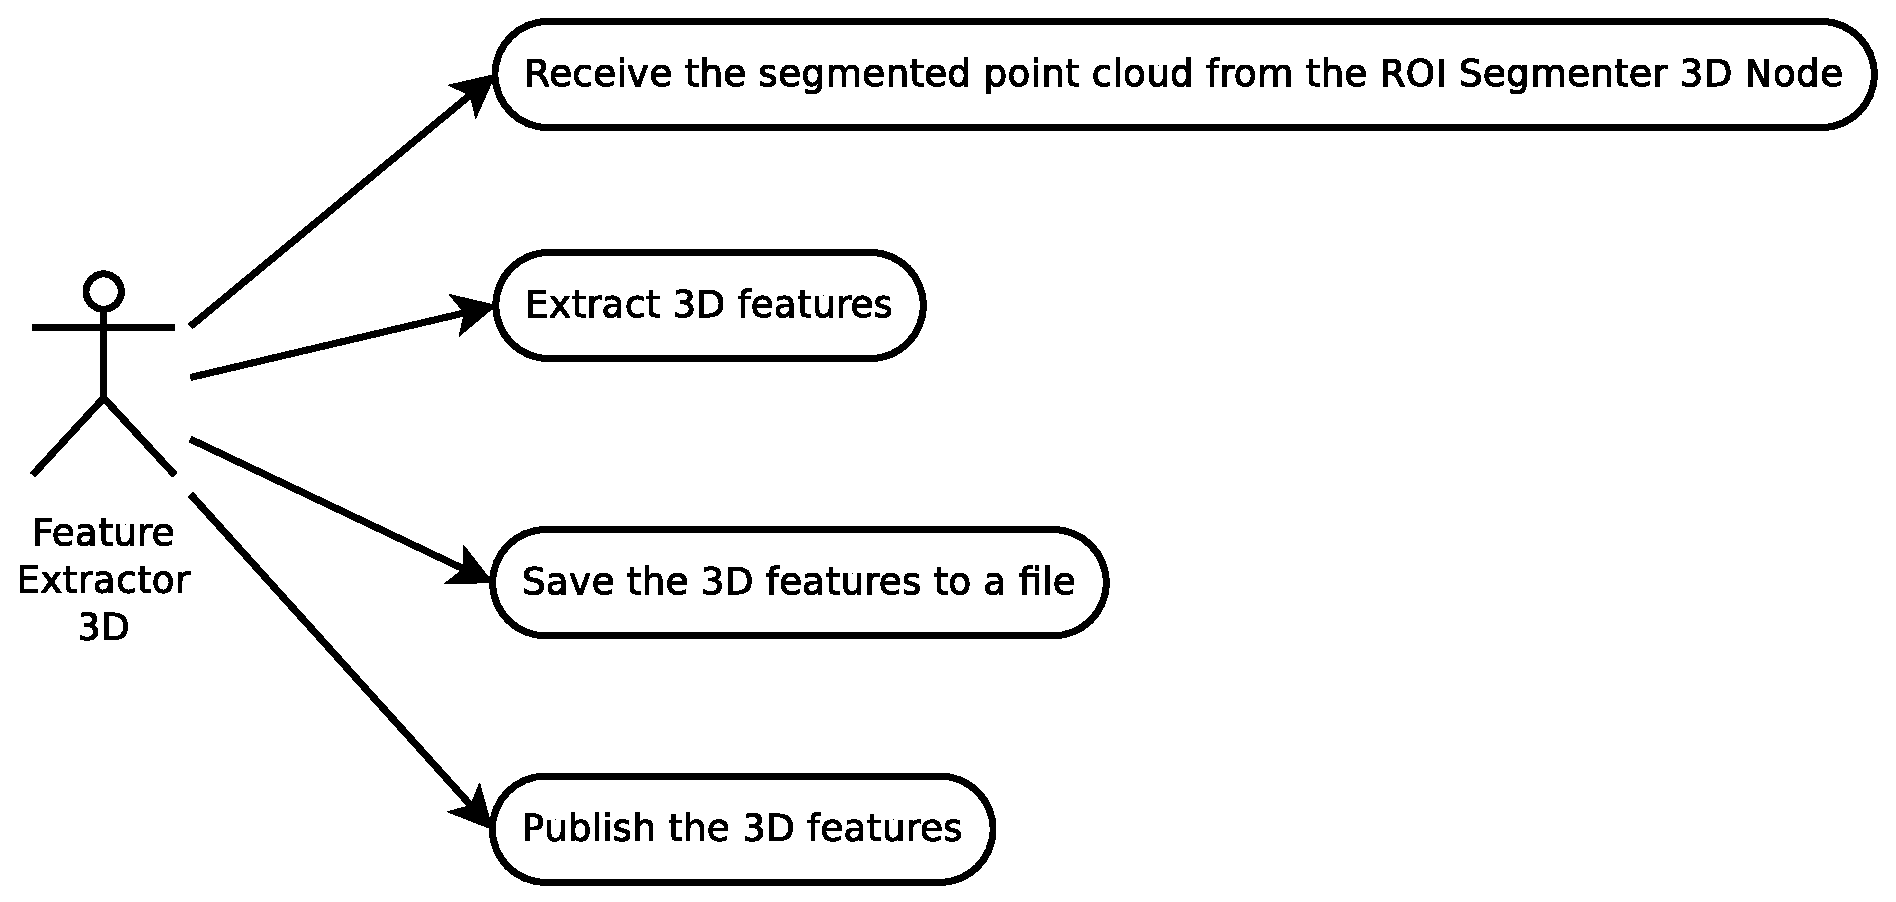
\includegraphics[scale=0.4]{img/diagrams/uc_feature_extractor_3d.eps}
			\caption[Use case diagram Feature Extractor 3D node]{Use Case diagram of the Feature Extractor 3D node}
		\label{uc_fe3d}
	\end{figure}

%%\newpage

\subsubsection{Event Handler node}

	As it was previously stated, in order to interact with the software some gestures were defined. This is the module that detects those gestures and switches accordingly to the corresponding event. This is the node responsible of detecting the different events that can appear in the system. 
	\\
	Figure \ref{node_event} shows the different Connectivity graph of the node. 
		\begin{figure}[H]
			\begin{center}
			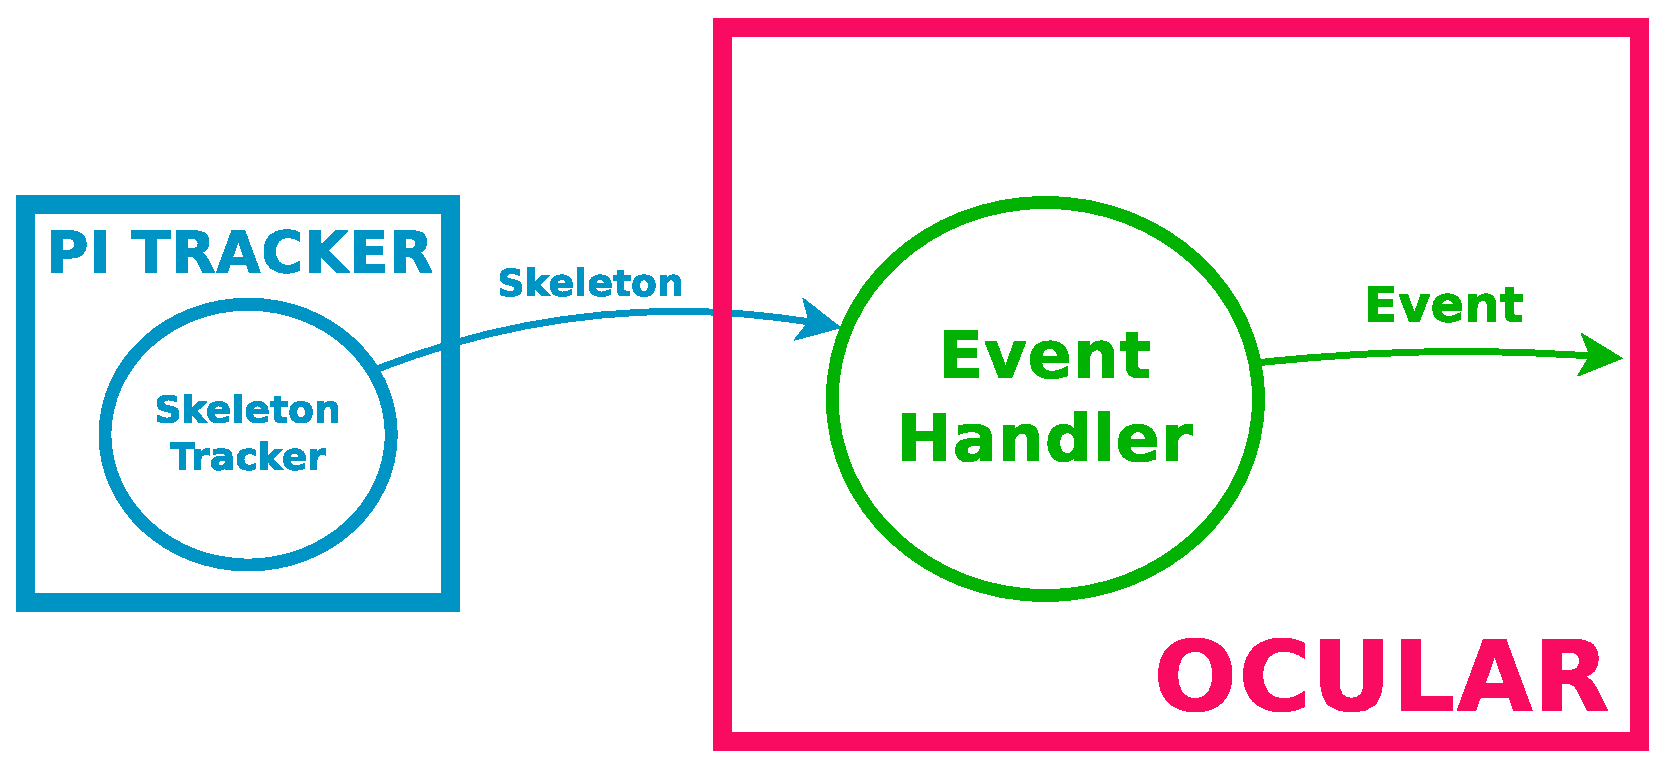
\includegraphics[width=0.5\linewidth]{img/diagrams/node_event.eps}
			\caption[Event Handler 3D node I/O]{Connectivity graph of the Event Handler node.}		
			\label{node_event}
			\end{center}
		\end{figure}
	The input of the system is the skeleton message that is obtained from the third-party package pi\_tracker. This message contains the information of all the joints of the user. The information is screened to detect the height at which each hand is located. The one that is the highest is the one being used in the software. Afterwards, the distance between the body and the chosen hand is computed. When that distance is similar to the distance of the user's arm, the event triggered is "learn". If, otherwise, the hand is located close to the body, the event that is published to the output topic is "recognize". 
	\\

	The distance that triggers the modes is proportional to the distance between the user and the RGB-D sensor in order to obtain a range of use of the software higher. 
	Figure \ref{uc_event} is a diagram with the use case of the node. 
	\begin{figure}[H]
		\centering
			\includegraphics[scale=0.4]{img/diagrams/uc_event_handler.eps}
			\caption[Use case diagram Event Handler node]{Use Case diagram of the Event Handler node}
		\label{uc_event}
	\end{figure}

%%\newpage

\subsubsection{Learner-Recognizer node}
\label{learner_recognizer}

	This node implements the state machine depending on the events recognized by the event handler node. If the event received is "learn", the learning sequence starts. If the event is "recognize", the recognize sequence is triggered. 
	\\

		\begin{figure}[H]
			\begin{center}
			\includegraphics[width=0.5\linewidth]{img/diagrams/node_lr.eps}
			\caption[Learner-Recognizer node I/O]{Connectivity graph of the Learner-Recognizer node.}		
			\end{center}
						\label{node_lr}

		\end{figure}

	The learn sequence consists in obtaining and storing the features both 2D and 3D and waiting a second allowing the user to move the object to capture a new view of it. 
	The dataset extracted is saved to a folder when the software is closed, to prevent possible lags in the runtime of the program. 
	Each view is saved separately. 
	This node loads the files that are still in the saving folder when the program is restarted. 
	\\

	The recognition sequence compares the newly obtained features both 2D and 3D with the ones that are stored in the dataset. 
	Afterwards, the result of the recognition for both types of descriptors are published in the output topic. 
	Figure \ref{uc_learner_recognizer} presents the use case diagram of the node. 

	\begin{figure}[H]
		\centering
			\includegraphics[scale=0.4]{img/diagrams/uc_learner_recognizer.eps}
			\caption[Use case diagram Learner-Recognizer node]{Use Case diagram of the Learner-Recognizer node}
			\label{uc_learner_recognizer}
	\end{figure}

%%\newpage


\subsubsection{System Output node}
\label{last_node}
	This nodes implements a buffer and a decision algorithm. 
	The input of the node is the object ID message from the Learner-Recognizer process as can be seen in figure \ref{node_output}.
	The node stores thirty values of instantaneous object estimations. 
	Since the Kinect runs at 30 frames per second, each second a new final object estimation appears. 
	The output of the node is the final object ID. 


		\begin{figure}[H]
			\begin{center}
			\includegraphics[width=0.5\linewidth]{img/diagrams/node_output.eps}
			\caption[System Output node I/O]{Connectivity graph of the System Output node.}		
			\label{node_output}
			\end{center}
		\end{figure}

	The decision is performed as follows. 
	The input to the algorithm are two vectors containing the 2D and 3D object estimations. 
	The frequency of each class is obtained. 
	Let us represent as $y'_{2D}$ and $y'_{3D}$ the vectors containing in each element the frequency of the object with $object_id = element$. 
	Both informations are combined in one vector called $y'$. 
	\\
	\begin{center}
	$y'=0.6*y'_{2D}+0.4*y'_{3D}$
	\end{center}
	More importance is being given to the 2D estimations since the 2D descriptors are more robust than the 3D ones. 
	The estimated final object id ($Y$) is obtained as the vector element that has the highest value. 
	\\
	\begin{center}
		$Y'= argmax(y')$
	\end{center} 
	This number $Y$ is the output of this whole system. 
	\\
	Figure \ref{uc_output} shows the use case diagram of this node. 

	\begin{figure}[H]
		\centering
			\includegraphics[scale=0.4]{img/diagrams/uc_system_output.eps}
			\caption[Use case diagram System Output node]{Use Case diagram of the System Output node}
			\label{uc_output}
	\end{figure}
 
\newpage
\subsection{Topics}
\label{topics}

	The topics are the channels that communicate the nodes in the ROS framework. All the nodes in the software are constantly obtaining messages from the input topics and publishing the results of their computation to the output ones. 
	\\

	In this section a relation of all the topics used in the software is presented. 


	\paragraph{Hand location}\mbox{} \\

	The complete path of this node in the code is: /TFG/CONVERTER/hand\_location. The messages published in this node are the custom HandLoc message. It specifies the location of both user's hands in the space. 
	\\

	\paragraph{Event}\mbox{} \\

	This node is filled by the node event\_handler. The message used by this node is the custom message TFG/EventHandler. The full name of this topic is /TFG/EVENTHANDLER/event. 

	\paragraph{Descriptors 2D}\mbox{} \\

		The complete name is /TFG/FE2D/descriptors2D. In this topic the Feature Extractor 2D node publishes the matrix of descriptors extracted from the segmented image. To this topic the Learner Recognizer node is subscribed in order to obtain those descriptors.  \\

	\paragraph{Descriptors 3D}\mbox{} \\

		In this topic the Feature Extractor 3D publishes the descriptors of the segmented point cloud. The Learner Recognizer node is subscribed to it. 
		The complete path to the topic is /TFG/FE3D/descriptors3D.\\


	\paragraph{Segmented image}\mbox{} \\

		The path  is /TFG/ROI2D/segmented\_image. In this topic the  ROI Segmenter 2D node publishes its output, the image with the region of interest. To this topic the Feature Extractor 2D is subscribed. \\


	\paragraph{Image with keypoints}\mbox{} \\

		The topic's name is /TFG/ROI2D/segmented\_image\_with\_keypoints. This topic is filled with images showing the segmented 2D ROI with the keypoints drawn on it. The node that publishes this data is FeatureExtractor2D. The topic is intended for visualization and troubleshooting purposes. \\

	\paragraph{Segmented coordinates}\mbox{} \\

		This topic is used to publish the information of the ROI location transformed to pixels. The topic is filled by the ROI Segmenter 3D node and the ROI Segmenter 2D node is subscribed to it. 
			\\
		The complete path of the topic is /TFG/ROI3D/segmented\_coordinates\_px. 

	\paragraph{Segmented pc}\mbox{} \\

		The present topic contains the messages with the segmented point clouds. It is filled by the ROI Segmenter 3D node as well and the Feature Extractor 3D node is subscribed to it. It is also possible to visualize using rviz or other point cloud visualization software the segmented point cloud. 
		\\

		The complete path to the topic is /TTFG/ROI3D/segmented\_pc.


	\paragraph{Object id}\mbox{} \\

		The name of the topic is /TFG/object\_id. This is the output of the system. The topic is filled by a custom message that contains information about the identification number of the recognized object and the grade of certainty in the recognition.\\

		Currently, the topic is only used in order to create a small feedback environment with the user. As part of the future work, another node could be developed to complete a natural interface with the user. This node would allow to give the learned object a name by talking to the software and in turn the code would output the recognized object as audio. For more information please read section \ref{conclusions}.

\newpage
\section{Software messages}
\label{software_messages}

% \newpage
% \subsection{Usage}
\label{usage}

In the present section the compilation and installation instructions of the software are presented as well as the usage instructions. 

\subsubsection{Operating System}
This project uses the ROS framework to compile and run. Since ROS is only available for Linux OS, this type of operating system should be installed in the computer used to run the code. 


\subsubsection{Software needed}
In order to use the software developed in this bachelor's thesis, the following packages are needed. 
\subsubsection{ROS}
The Robotic Operating System is used within the software as the means of communication between the different nodes. Also, different ROS packages are used to provide the input information to the system. Hence, it is needed to install it. 
\\

The code has been tested with the Groovy or Indigo ROS distributions. For installation instructions the webpage http://ros.org provide numerous tutorials. 
\\

Between those distributions there is another one which is called Hydro. For this particular one the code has not been tested but since there are no major changes between Hydro and Indigo, the code used for this latter should compile without problems. 


\subsubsection{ROS package: openni\_camera / freenect\_camera}
These packages are the drivers of the kinect. They should be installed via command-line, which is the recommended, or downloading and compiling the source code. 
\\

In order to install these packages using the terminal, please introduce the following commands: 
\\

sudo apt-get install ros-<distro>-openni\_camera
\\

sudo apt-get install ros-<distro>-freenect\_camera
\\

Replace the <distro> word by the distribution currently installed on your computer, Groovy or Indigo, in lower case. 



\subsubsection{ROS package: openni\_launch / freenect\_launch}
These package needs to be launched in parallel with the code provided in this bachelor's thesis. As the previous ones, they can be downloaded using the terminal or compiling the source code. 
\\

In oder to install them using the command-line please enter the following on it: 
\\

sudo apt-get install ros-<distro>-openni\_launch
\\

sudo apt-get install ros-<distro>-freenect\_launch
\\

This commands install the ROS package in the default directory in which the ROS libraries are stored, usually /opt/ros/<distro>. 



\subsubsection{ROS package: pi\_tracker}
The pi\_tracker package is needed in order to retrieve the position of the user's skeleton. Unfortunately it is not available for command-line installing. This means that the code must be downloaded and compiled in order to be used. 
\\

To do so, the source code must be downloaded into the ROS workspace already created. The source code might be found on the web-page: http://github.com/pi\_tracker. 
\\

For further details on how to download and install ROS packages using the source code please read the following section. 

\subsection{ROS packages source code compilation}
The first thing needed is the ROS workspace. Depending on the ROS distribution, this workspace might be a catkin workspace or a rosbuild workspace. 
\\

Catkin and rosbuild are two methods implemented by ROS to organize the code and to compile it. Both use CMAKE below to compile the code, with specific arguments for different compilation options. 
\\

\subsubsection{Catkin workspace}
The first thing needed is to create a folder for the workspace and a src folder within the first one. This can be done through the interface or using the following command in a terminal: 
\\

mkdir -p <path-to-workspace>/<name-of-workspace>/src\\

Then, insert the following command or open a terminal inside the src folder: \\

cd <path-to-workspace>/<name-of-workspace>/src\\

Finally, in order to initiate the catkin workspace, type: \\

catkin\_init\_workspace\\

This creates an empty workspace. The different packages must be located inside the src folder. \\

In order to build the workspace, move to the upper folder of your workspace and insert the following command: \\

catkin\_make\\

This compiles all the packages within the catkin workspace. In order to use the packages inside this folder, it is necessary to source the setup bash files inside the devel folder. This overlays the workspace on top of your ROS environment. Enter the following command: \\

source <path-to-workspace>/<name-of-workspace>/devel/setup.bash\\




\subsubsection{Rosbuild workspace}
First, introduce the following command in order to create the workspace folder: \\

mkdir -p <path-to-workspace>/<name-of-workspace> \\

Then, in order to create the workspace the rosws command is needed, which is not installed by default. It can be downloaded using the Ubuntu package manager introducing the following in a terminal: \\

sudo apt-get install python-rosinstall\\

Now it is possible to create the workspace using: \\

rosws init <path-to-workspace>/<name-of-workspace> /opt/ros/<ROS-distro>\\

In a rosbuild workspace the packages are located within the sandbox folder. To create it and set it insert the following: \\

mkdir <path-to-workspace>/<name-of-workspace>/sandbox\\

rosws set  <path-to-workspace>/<name-of-workspace>/sandbox\\

Whenever the entries in the workspace suffer changes, it is necessary to re-source the setup file inside the workspace to make sure the updated ROS\_PACKAGE\_PATH is used. In order to source the workspace introduce this line in a terminal: \\

source <path-to-workspace>/<name-of-workspace>/setup.bash\\




\subsection{OCULAR compilation}
The source code might be found in the repository : http://github.com/irenesanznieto/ocular. There are two branches within that code, one for the Groovy and the other for the Indigo distributions. 
\\




\subsection{Launch files}

\subsection{Run the code}







%%% METHODS
\part{Methods}
\label{methods}

%\addcontentsline{toc}{part}{Introduction}
\part{Introduction}


%	
\section{Motivation}

Technology has evolved enormously in the past years. 
% In particular, robotics has changed and moved from controlled spaces such as factories to human inhabited spaces. 
% In section \ref{context} the reasons behind this shift in the robot's location and function were presented. 
% It was also estated that the importance of the perception systems augmented with the inclusion of robots in human-inhabited areas. 
% % This fact increases the importance of the perception systems being integrated. 
% The correct recognition of objects, persons, areas and situations is key for assistive and social tasks. 
Nowadays most of the robots being developed are only able to recognize a small part of their environment. 
% Most computer vision systems are currently used to navigate between points or to locate certain objects and grasp them. 
The decision algorithm of the robots is normally based on the instructions received from the user. 
Those commands are usually given by voice or inputting the desired task on a certain User Interface (UI).
\\

% For the robots to act as aiding personnel to take care of elder or sick people, the evolution of this decision algorithm is crucial. 
The algorithm decision of the robots must be upgraded if they are to perform tasks in a human inhabited area. %act as aiding personnel to take care of elder or sick people. 
They must be able to respond to commands, but also be aware of their environment and respond autonomously to it. 
% As an example, robots must be able to recognize the danger involved in certain objects or situations. 
% Also, they should perceive the environment and the interactions between humans to discern if, for example, they are arguing or if the conversation is not a beneficial one for the patient. 
% This latter example may be seen in the case of an anorexic person who is talking about food and weight with another person. 
% Then, the robot may intervene changing the subject subtly or trying to end the conversation. 
When this change has occurred, the robots may successfully perform the assistive tasks now reserved only to humans. 
But there is still a long way to research, mainly around the perception of the environment. 
The investment needed for its development is now being held due to the recession that appeared in the late 2000s decade, whose effects are nowadays still present. 
Nevertheless, this lack of funding might be mitigated using research, open data and open-source code. 
\\

I strongly believe in the ideals presented by the Open Source Initiative. 
This project is intended to be an open source code that can be a building block for other researchers that work on robot perception.
There are various scientists that have already studied the importance of the objects around the human in the action recognition. 
For example, in \cite{Delaitre}, a study of the human-object interaction in still images was performed in order to relate those objects to actions. 
	This relation between object and action may also be seen in \cite{Fathi}, in which wearable cameras are used to retrieve the input. 
	The objects being hand-held are recognized and the action associated to them is learned. 
	In this thesis I present a system that allows to easily learn and recognize hand-held objects in real time. 
	It is intended to be the previous step to the association between the object and the action. 



% The economic situation described above forced many experienced professionals to trying their luck creating start-ups. Many of the ideas of those enterprises are having nowadays a huge impact on the society. 
% \\

% One of these open-source projects that appeared was the low-cost 3D printers. These machines have changed the manner of investigating many fields, since they allow to design different pieces easily and have a 3D reproduction in a few hours. 
% \\

% Initially, they were used in investigation and more specifically in robotics, but now they are used in many different fields. Among those fields, there are medicine, construction or even food making. 
% \\

% In medicine, they have been a revolution since they allow to create customized and precise pieces in very few time. They have been used for prosthesis and implants for persons of various ages, even for babies. In the prosthesis fields in particular, the 3D printing technology is being a complete revolution. Before, the prosthesis were very expensive and permitted only fixed movements and combinations. The adaptations to each individual were made in the final product itself, trying to make it as comfortable as possible for the wearer. Nowadays, the prosthesis are customized for each patient, reducing the inconveniences and increasing their usability. Also, they can be easily and cheaply adapted for children as an example, who are still experimenting many changes in their bodies. They are much cheaper than they were before, and everyone with a 3D printer may construct one. 
% In order to 3D print a piece a file with its description is needed. There are many web-pages that store open-source designs that ranges from decoration models to complex prosthesis. This fact is decisive because there is not needed a huge amount of knowledge or money to improve the life quality of a person using these technologies. 
% \\

% There are numerous open-source projects and developers that put in common their knowledge to improve the technology being used. I have used many of them in the previous years, to learn about 3D printing, robotics or programming among other fields. 
% \\

% It is a fact that acquiring knowledge would be much difficult if the Open Source initiative has not been invented. This impulsed me towards developing something useful and that could be used by other people. The idea of creating a software that could be used in robotics investigation but also help people at the same time. 
% \\[0.5cm]

% Many of the projects are aimed at aiding physically impaired people, creating sternal skeletons and robotic arms that could aid them. But a personal fact led me to realize that visually impaired people were not having as much attention. The applications developed for them are still rough to use and also it is difficult for a grown person to develop his remaining senses to supply the information lost. 
% \\

% Besides, in the robotic field new lines of investigation have appeared. The social robots are now a reality and in the near future we will interact with them everyday. In order to understand the human behavior, the recognition of the objects being handled by them is crucial. 
% \\[0.5cm]


% Computer vision has experience an important improvement in the last years through the upgrade of the hardware and software that compose it. The hardware such as acquisition elements (cameras, depth sensors, etc) and computing elements (PCs or other programmable devices) have experienced a rapid advance in the past years. It allowed to process more data that is now obtained more accurately and with less noise. This increase in the computing power of the equipment created a possibility of introducing more complex libraries and frameworks and even operating systems. 
% \\

% Now, the technology is available to solve the problems presented, the aid of visually impaired people and the introduction of new information in the social robotics field. This is how the idea behind this thesis appeared: the creation of a modular software that implements an in-hand object recognition algorithm. 
 
%	%\addcontentsline{toc}{chapter}{Socio-economical context}
\section{Socio-economical context}

%Socio-economic - relating to both social and economic factors (social groups and the class system for example)
%Context - The circumstances/environment/events surrounding a specific thing. 



%	%\addcontentsline{toc}{chapter}{Future applications}
\chapter{Future applications}
	% future applications



\chapter{Introduction}
This bachelor's thesis consists on a software that implements an in-hand object learning and recognition using 2D and 3D information. 
\\

The code is Open-Source and it was designed to be running inside a robot. The idea is to create a new stand-alone module that could be included in every robot using ROS and a kinect or other RGB-D sensor. This way, having different modularized functionalities it could be possible to create a customized robot in a few seconds, just importing packages and compiling them. 
\\[1cm]

\chapter{Context and motivation}
In the past fifteen years, there has been a change in the perception of the knowledge and whether it should be restricted using patents or not. Most of the scientific community now supports the open source initiative and this has caused a huge increase on the investigation field. \\



The idea of creating common software, of aiding other investigators to easily replicate the work already done and continue from that point instead of "reinventing the wheel" started in the past century. In 1998 the Open Source Initiative (OSI)\cite{osi} was formed, and its definition is recognized as the standard. According to them, "Open source does not just mean access to the source code. The distribution terms of open-source software must comply with the following criteria: Free Redistribution, Source Code, Derived Works, Integrity of The Author's Source Code, No Discrimination Against Persons or Groups, No Discrimination Against Fields of Endeavor, Distribution of License, License Must Not Be Specific to a Product, License Must Not Restrict Other Software,  License Must Be Technology-Neutral"\cite{osi_def}. 
\\

It is my believe that Open Source is critical in the development of new knowledge and not only in the Software field, but in all the science and technical disciplines. This is how the idea of increasing that common pool of tools with another one that might be useful appeared. 
\\
%\begin{wrapfigure}{r}{0.3\textwidth}
%	\centering
%   \includegraphics[width=0.25\textwidth]{img/intro/open_source.eps}
%	\caption[Open Source Initiative Logo]{Open Source Initiative Logo}
%\end{wrapfigure}

\begin{figure}[h]
	\begin{center}
    \includegraphics[scale=0.2]{img/intro/open_source.eps}
	\caption[Open Source Initiative Logo]{Open Source Initiative Logo}
	\end{center}
\end{figure}


It is noticeable the mark that Open Source has throughout the project. From the libraries being used in it to the Robotic Operating System of which this project is but another package. All of them are Open Source. Also, the tutorials, examples and different web-pages with useful comments and aids for those who are learning has been critical in this project's development. Nothing of this could have been possible without the idea of Open Source code. 
\\

%Apart from the want of making useful Open Source code, there remains another motivation unexplained. That is, the specific subject of this project. 
\\

%The bad economic context that exist nowadays has forced the different areas of the society to investigate new technologies that has a lower cost. 
%Nowadays, advances regarding robotics appear everyday, and technologies such as 3D printing are having a tremendous impact in the society. Thanks to this instruments, now it is possible and relatively easy to customize prosthesis and also much affordable than it was before. 
%\\

%Robotics is a field that is experiencing a huge impulse currently. And more specifically, Open Source robotics is growing rapidly. 
%\\

One of the open-source projects that appeared with this new way of thinking was the low-cost 3D printers. These machines have changed the manner of investigating in robots, since they allow to design them easily and have a 3D reproduction in a few hours. 
\\

But they are used not only in robots, but also in medicine and many other fields. In medicine, they have been a revolution since they allow to create customized pieces in very few time. They have been used for prosthesis and implants for persons of various ages, even for babies. 
\\

Before, the prosthesis were very expensive and permitted only fixed movements and combinations. The adaptations to each individual were made in the final product itself, trying to make it as comfortable as possible for the wearer. Nowadays, the prosthesis are customized for each patient, reducing the bothers for them and increasing their usability. Also, they can be easily and cheaply adapted for children as an example, who are still experimenting many changes in their bodies. They are much cheaper than they were before, and everyone with a 3D printer may construct one. 
\\

Of course, in order to 3D print a piece a file with its description is needed. There are many web-pages that store open-source designs that ranges from decoration models to complex prosthesis. This fact is decisive because there is not needed a huge amount of knowledge or money to improve the life quality of a person using these technologies. 
\\

There are numerous open-source projects and developers that put in common their knowledge to improve the technology being used. I have used many of them in the previous years, to learn about 3D printing, robotics or programming among other fields. 
\\

The fact that previously I have developed other projects involving designing and constructing 3D-printed wheeled robots gave me the idea of developing a new package for different robots that allowed to easily obtain new functionalities.One of the most interesting fields that can be used in virtually all types of robots is Computer Vision. 
\\

Computer vision has experience an important improvement in the last years through the upgrade of the hardware and software that compose it. The hardware such as acquisition elements (cameras, depth sensors, etc) and computing elements (PCs or other programmable devices) have experienced a rapid advance in the past years. It allowed to process more data that is now obtained more accurately and with less noise. This increase in the computing power of the equipment created a possibility of introducing more complex libraries and frameworks and even operating systems. 
\\

But Computer Vision is an ample area, why choosing object recognition? The project being developed is intended to be useful, not just a mere hobby. It occurred to me that apart from being useful in the interaction with robots and cognitive robots more particularly, this software could be used with visually impaired people, as an example. Mainly, with people that had a sudden loss of vision and that is not used to detect the objects by its shape, or cannot differentiate them by the contour. 
\\

In summary, the software developed is open-source and is intended as a useful package for visually impaired persons, as well as for its integration within a robotic system. 

\newpage
%\addcontentsline{toc}{part}{Introduction}
\part{Introduction}


%	\input{intro/motivation} 
%	\input{intro/context}
%	\input{intro/uses}	% future applications



\chapter{Introduction}
This bachelor's thesis consists on a software that implements an in-hand object learning and recognition using 2D and 3D information. 
\\

The code is Open-Source and it was designed to be running inside a robot. The idea is to create a new stand-alone module that could be included in every robot using ROS and a kinect or other RGB-D sensor. This way, having different modularized functionalities it could be possible to create a customized robot in a few seconds, just importing packages and compiling them. 
\\[1cm]

\chapter{Context and motivation}
In the past fifteen years, there has been a change in the perception of the knowledge and whether it should be restricted using patents or not. Most of the scientific community now supports the open source initiative and this has caused a huge increase on the investigation field. \\



The idea of creating common software, of aiding other investigators to easily replicate the work already done and continue from that point instead of "reinventing the wheel" started in the past century. In 1998 the Open Source Initiative (OSI)\cite{osi} was formed, and its definition is recognized as the standard. According to them, "Open source does not just mean access to the source code. The distribution terms of open-source software must comply with the following criteria: Free Redistribution, Source Code, Derived Works, Integrity of The Author's Source Code, No Discrimination Against Persons or Groups, No Discrimination Against Fields of Endeavor, Distribution of License, License Must Not Be Specific to a Product, License Must Not Restrict Other Software,  License Must Be Technology-Neutral"\cite{osi_def}. 
\\

It is my believe that Open Source is critical in the development of new knowledge and not only in the Software field, but in all the science and technical disciplines. This is how the idea of increasing that common pool of tools with another one that might be useful appeared. 
\\
%\begin{wrapfigure}{r}{0.3\textwidth}
%	\centering
%   \includegraphics[width=0.25\textwidth]{img/intro/open_source.eps}
%	\caption[Open Source Initiative Logo]{Open Source Initiative Logo}
%\end{wrapfigure}

\begin{figure}[h]
	\begin{center}
    \includegraphics[scale=0.2]{img/intro/open_source.eps}
	\caption[Open Source Initiative Logo]{Open Source Initiative Logo}
	\end{center}
\end{figure}


It is noticeable the mark that Open Source has throughout the project. From the libraries being used in it to the Robotic Operating System of which this project is but another package. All of them are Open Source. Also, the tutorials, examples and different web-pages with useful comments and aids for those who are learning has been critical in this project's development. Nothing of this could have been possible without the idea of Open Source code. 
\\

%Apart from the want of making useful Open Source code, there remains another motivation unexplained. That is, the specific subject of this project. 
\\

%The bad economic context that exist nowadays has forced the different areas of the society to investigate new technologies that has a lower cost. 
%Nowadays, advances regarding robotics appear everyday, and technologies such as 3D printing are having a tremendous impact in the society. Thanks to this instruments, now it is possible and relatively easy to customize prosthesis and also much affordable than it was before. 
%\\

%Robotics is a field that is experiencing a huge impulse currently. And more specifically, Open Source robotics is growing rapidly. 
%\\

One of the open-source projects that appeared with this new way of thinking was the low-cost 3D printers. These machines have changed the manner of investigating in robots, since they allow to design them easily and have a 3D reproduction in a few hours. 
\\

But they are used not only in robots, but also in medicine and many other fields. In medicine, they have been a revolution since they allow to create customized pieces in very few time. They have been used for prosthesis and implants for persons of various ages, even for babies. 
\\

Before, the prosthesis were very expensive and permitted only fixed movements and combinations. The adaptations to each individual were made in the final product itself, trying to make it as comfortable as possible for the wearer. Nowadays, the prosthesis are customized for each patient, reducing the bothers for them and increasing their usability. Also, they can be easily and cheaply adapted for children as an example, who are still experimenting many changes in their bodies. They are much cheaper than they were before, and everyone with a 3D printer may construct one. 
\\

Of course, in order to 3D print a piece a file with its description is needed. There are many web-pages that store open-source designs that ranges from decoration models to complex prosthesis. This fact is decisive because there is not needed a huge amount of knowledge or money to improve the life quality of a person using these technologies. 
\\

There are numerous open-source projects and developers that put in common their knowledge to improve the technology being used. I have used many of them in the previous years, to learn about 3D printing, robotics or programming among other fields. 
\\

The fact that previously I have developed other projects involving designing and constructing 3D-printed wheeled robots gave me the idea of developing a new package for different robots that allowed to easily obtain new functionalities.One of the most interesting fields that can be used in virtually all types of robots is Computer Vision. 
\\

Computer vision has experience an important improvement in the last years through the upgrade of the hardware and software that compose it. The hardware such as acquisition elements (cameras, depth sensors, etc) and computing elements (PCs or other programmable devices) have experienced a rapid advance in the past years. It allowed to process more data that is now obtained more accurately and with less noise. This increase in the computing power of the equipment created a possibility of introducing more complex libraries and frameworks and even operating systems. 
\\

But Computer Vision is an ample area, why choosing object recognition? The project being developed is intended to be useful, not just a mere hobby. It occurred to me that apart from being useful in the interaction with robots and cognitive robots more particularly, this software could be used with visually impaired people, as an example. Mainly, with people that had a sudden loss of vision and that is not used to detect the objects by its shape, or cannot differentiate them by the contour. 
\\

In summary, the software developed is open-source and is intended as a useful package for visually impaired persons, as well as for its integration within a robotic system. 

\newpage
\input{intro/intro} 
\newpage
\input{intro/thesis_structure}
 
\newpage
\addcontentsline{toc}{chapter}{Thesis structure}
\chapter*{ Thesis structure}


%\addcontentsline{toc}{chapter}{Hardware}
\section{Hardware}



 
%%%%%%% INTRODUCTION %%%%%%
%%\addcontentsline{toc}{section}{Introduction}
%\section{Introduction}
The advance in the computer vision discipline is greatly linked with the development in the hardware. The main components of a computer vision system are the following: 

\begin{itemize}
	\item{Power Supply: } Device needed by the other components in order to work. 
	\item{Acquisition device: } Device that captures the world and represents it as an array of data. That data can be two or three dimensional. 
	\item{Processing unit:} Receives the information from the acquisition device and processes it. It is usually programmable. Nowadays the most used processing units are PCs. 
	\item{I/O unit: } Serves as a bridge between the acquisition device and the processing unit if needed. 

\end{itemize}

In this chapter the state of the art of the different acquisition devices is going to be presented. 

%%%%%% ACQUISITION DEVICES %%%%%%
%\addcontentsline{toc}{section}{Acquisition devices}
\subsection{Acquisition devices}
There are different acquisition devices being used in the computer vision field. They are usually classified depending on the output data they provide: 

\begin{itemize}
	\item{Cameras:}	The output data is two-dimensional. 
	\item{RGB-D sensors:} The output data is three-dimensional. 
\end{itemize}

The usage of one or another acquisition device depends on the application. The RGB-D sensors provide a higher number of information than the cameras. They reduce the ambiguities produced by the cameras when projecting the three-dimensional world into to dimensions. But also the RGB-D sensors output a higher amount of data. 
That is why, using three-dimensional information as the input of a software requires a higher-capacity processing unit than using two-dimensional data.



%%%%%% CAMERAS %%%%%%
%%\addcontentsline{toc}{section}{Cameras}
\subsection{Cameras}
\label{cameras}



%%%%%% RGB-D SENSORS %%%%%%
%\addcontentsline{toc}{section}{RGB-D Sensors or Natural Interaction Devices}
\subsection{RGB-D Sensors or Natural Interaction Devices}
\label{rgb-d}
%\addcontentsline{toc}{subsection}{History}
\subsubsection{History}

Computer vision is a field that needs specific hardware to retrieve a description of the world. This description has been done for a number of years in two dimensions. But this changed when the first version of an affordable RGB-D sensor appeared in 2010: the Kinect. This project uses a Kinect RGB-D sensor as the input of the system.
\\

This sensor was designed to be used in games, but developers soon realized the huge potential of the hardware for Computer Vision.  
Now, instead of a two-dimensional information as an input it was possible to have three-dimensional information. 
\\

The Microsoft corporation released the SDK (Software Development Kit) on June, 2011 \cite{kinectSDK}.
\\

But one year before, PrimeSense released their open source drivers and motion tracking middleware called NITE\cite{NITE}. 
PrimeSense is a company that manufactures RGB-D sensors and, in fact, the Kinect is based on their depth sensing reference. Hence, the software released by PrimeSense worked with the Kinect as well. 

From that time on, the OpenSource software related with the kinect has increased as well as the different models of RGB-D sensors available in the market.
In November 2010 OpenNI was created. Openni is an open-source software framework that can read the data from RGB-D sensors \cite{openni}.  

%\addcontentsline{toc}{subsection}{How does the Kinect work?}
\subsubsection{RGB-D sensors in this project}


% \section{Code testing}
% The code has been designed to be easily tested. The communication and ROS functions are separated from the actual computing of the nodes. 
% \\

% The class structure of the code is hence as follows: the base class performs the operations needed by the node and there exists a wrapper class that implements the publishing and subscribing to the different nodes. \\

% In the actual application, it is an object of this latter wrapper class the one that is created. 
% \\

% This structure easies the testing, since the first testing level is done in the base classes and the second and third on the wrapper classes.
% \\

% For further details about the tools used to perform the testing please read the section \ref{testing}.
% \\

% In the following sections the libraries being tested in each level are presented. 

% 	\subsection{First level: Library unit test}
% 		The library used to perform this unit testing is gtest. More information about that library may be found in the section \ref{gtest}.
% 		In this level, the base classes are tested. Those classes are located in the src/libraries/libraries directory. The tests performed are: 
			% \subsubsection{Converter Test}

			% \subsubsection{ROI Segmenter 2D Test}

			% \subsubsection{ROI Segmenter 3D Test}

			% \subsubsection{Feature Extractor 2D Test}

			% \subsubsection{Feature Extractor 3D Test}

			% \subsubsection{Algorithm2D Test}

			% \subsubsection{Algorithm3D Test}

			% \subsubsection{Event Handler Test}

			% \subsubsection{Data Parser Test}

	% \subsection{Second level: ROS node unit test}
	% 	In order to perform this testing level a library unit test and the rostest tool are needed.The rostest tool is explained in detail in the following \ref{rostest} section.\\

	% 	The tests developed in this level are the following: 

	% \subsection{Third level: ROS node integration / regression test}
	% 	In order to perform a third-level testing, both a unit testing library and the rostest tool are needed. In this project, the tests implemented of this level are the following: 


\section{Computing performance evaluation}

	This section presents the tests that I performed to evaluate the computing performance of the system. 
	The main objective of these tests is to demonstrate that the system is able to operate in real-time, so it can be used while interacting with a human.
	The topics and the nodes of the system are being evaluated measuring their main characteristics. 
	The nodes computing performance is obtained from their CPU and RAM consumption. 
	The topics are the means of communication of the nodes. 
	In the topics the messages are published and more than one node can subscribe to each topic and hence access to those messages. 
	In this evaluation, the total bandwidth and publishing rate of the topics are measured. 

	% The performance testing is used to benchmark the system.
	% There are different items of the system that are tested. 
	% Since the code is divided in nodes, the performance of each node is evaluated. 
	% The sum of those performances gives the total package benchmarking. 
	% Also, the topics used to communicate the nodes are evaluated. 
	% The details may be found in the sections below. 
	% \\[0.5cm]
	% \begin{itemize}
		% \item{\textbf{Nodes' CPU and RAM usage}}
		% \\
		\subsection{Nodes' CPU and RAM usage}

		The CPU and RAM consumption of each node was measured. 
		The total usage of the whole system can be calculated summing the individual consumptions. 
		In section \ref{results}, the results of this evaluation are presented. 
		The CPU and RAM usage are presented in percentage. 
		% The package developed is composed of different nodes. 
		% Since the computing is distributed, each node has different CPU and RAM usages.
		% That is why in these experiments the particular behavior of each node is evaluated. 
		% The CPU and RAM usages are given in percentages. 
		% The computer used has a i7 processor. 
		% This means that it has four processing cores that uses two threads each, totaling eight virtual cores. 
		% The CPU usage is hence represented from the 0 to the 800\%.
		% The RAM usage is represented from 0 to 100\%.
		% % \\[0.5cm]

		% The whole package benchmarking is obtained summing the performances of the different nodes. 
		% This information is important to know the minimum specifications of the computer used in order to obtain a real-time response of the system.  

		% The results are being shown in section \ref{results} in a table as the one in figure \ref{node_model}.

		% \begin{figure}[H]
		% 		\begin{center}
		% 	    \includegraphics[scale=0.48]{img/tests/node_model.png}
		% 		\caption[Node benchmarking - Table model]{Node benchmarking - Table model}
		% 						\label{node_model}

		% 		\end{center}
		% \end{figure}

		% \item{\textbf{Topic network usage}}\\
		\subsection{Topic network usage}

		The computing performance tests also evaluate the topic bandwidth (BW) and frequency requirements. 
		The motivation of this evaluation is the following.
		ROS is a distributed system that allows spreading the computation across multiple machines. 
		This allows to create distributed computing systems where the robots carry low-power consuming computers and delegate the CPU intensive tasks to remote servers.	
		The drawback of this approach is that communicating machines consume network resources. 
		This is specially relevant for image or video tasks, which do consume great amounts of BW. 
		The need to evaluate the BW and frequency requirements of the system comes from this issue. 
		Therefore, the purpose of the topic network usage measurement is to evaluate if the system could be distributed across several machines.

		% The topics communicate the nodes and allow the exchange of information. 
		% The parameters that characterizes the topics are the bandwidth and the publishing frequency.
	
		% % \paragraph{Bandwidth}\mbox{}\\
		% The bandwidth parameter is the speed at which the data is transmitted. 
		% Its units are kilobytes per second. 
		% The ROS framework has a built-in command that allows to retrieve the maximum, minimum, mean and average bandwidth of a topic. 
		% % The results are presented in a table as the one in figure \ref{topic_bw_model}. 

		% \begin{figure}[H]
		% 		\begin{center}
		% 	    \includegraphics[scale=0.35]{img/tests/topic_bw_model.png}
		% 		\caption[Topic benchmarking - Bandwidth table model]{Topic benchmarking - Bandwidth table model}
		% 		\label{topic_bw_model}
		% 		\end{center}
		% \end{figure}
		% If there are network connectivity problems or rostopic cannot keep up with the publisher, the reported bandwidth might be lower than the actual one. 
		\\

		% \paragraph{Publishing frequency}\mbox{}\\
		The publishing frequency of a ROS topic is the number of messages published on it over time. 
		It is measured in Hz. 
		ROS provides a built-in command that is similar to the one above that returns the maximum, minimum and the standard deviation of the time between messages in seconds. 
		Also, it returns the average publishing frequency.  
		% A table like the one in figure \ref{topic_hz_model} is used to present the results.

		% \begin{figure}[H]
		% 		\begin{center}
		% 	    \includegraphics[scale=0.35]{img/tests/topic_hz_model.png}
		% 		\caption[Topic benchmarking - Publishing rate table model]{Topic benchmarking - Publishing rate table model}
		% 						\label{topic_hz_model}
		% 		\end{center}
		% \end{figure}
		% 	\end{itemize}

% \newpage

\section{Evaluation of the object recognition accuracy}
\label{accuracy_experiment}

	This experiment is designed to obtain data related to the accuracy of the system. 
	% In the following sections the conditions and parameters that affect the test are shown and explained as well as the testing procedure that is followed. 
	Sections \ref{setup}, \ref{set_of_objects}, \ref{procedure} and \ref{accuracy_measurement} explain the conditions and parameters that affect the experiment and also the testing procedure that has been followed. 
	%\\[0.5cm]

	% \subsection{Environment \& testing conditions}
		% The test is performed in a room with a crowded background , that is, a room without a blank background and with various objects at different depths.
		% The light source is located behind the RGB-D sensor, directly illuminating the user. 
		% The objects that conform the dataset are located next to the tester to facilitate the accessibility to them. 
	%	The test is performed in a room with uniform background and lightning. 


		%\\%[0.5cm]

	% \begin{figure}[H]
	% 	\begin{center}
	%     \includegraphics[scale=0.3]{img/testing_environment.eps}
	% 	\caption[Testing Environment]{Testing Environment}
	% 	\end{center}
	% \end{figure}

	\subsection{Experimental setup}
	\label{setup}
	The experiment was performed in a highly illuminated room with white walls. 
	The light was a mixture of natural light and artificial light coming from halogens.
	The experiment was performed at a distance of approximately 1.7 m from the RGB-D (Red, Green, Blue and Depth) sensor. 
	The background was composed of a white wall with a painting in the right side, a window in the left side and shelves in the middle-left part. 



	\subsection{Experimental set of objects}
	\label{set_of_objects}
		The objects being used in the experiment are common objects. 
		They can be seen in Figure \ref{dataset}.
		Using common objects allow to obtain more reliable experiment results, since they were obtained under working conditions. 
		Common objects are usually featureless. 
		That characteristic complicates the object recognition, since objects with rich textures usually generate more robust descriptors.
		In order to overcome this difficulty, different views of each object are obtained and compared when doing the matching. 
		Also, the introduction of both 2D and 3D features diminish the possibilities of false positives and false negatives. 

		\begin{figure}[H]
				\begin{center}
			    \includegraphics[width=\textwidth]{img/tests/dataset02.jpg}
				\caption[Experimental dataset]{Experimental dataset. From left to right: ball, skull, cup, mobile and calculator.}
				\label{dataset}

				\end{center}
		\end{figure}
	% \subsection{Dataset}


		%This is because the software is intended to be running in a social robot that needs to recognize the most used objects. 
		%Also, the other possible application of the software is as an aiding software for visually impaired persons. 
		%In this case it is a requirement the recognition of daily objects as well.  
		%\\
		% The ones being used in the present experiment may be seen in figure \ref{dataset}. 
	
		This particular dataset is conformed of objects that could be easily confused by a computer vision system using descriptors. 
		As an example, the 3D shape of the ball and the skull is very similar, a fact that would lead to akin 3D descriptors. 
		Also, the cup, the bottle and the mobile have comparable 2D texture. 
		\\%[0.5cm]

	\subsection{Experimental procedure}
	\label{procedure}

		The testing is performed following this sequence. 
		% First, the tester shows the first two objects that are going to be learned. 
		% Afterwards, the recognition mode is tested identifying and storing in a file the output of the matching for both 2D and 3D. 
		% \\

		% Then, another new object is learned and again the recognition is tested. 
		% This sequence is iterated until there are no new objects to be learned. 
		% \\

		% The reason behind this incremental learning is to observe the differences on the effectiveness and the benchmarking of the system when the dataset size changes. 
		% \\

		First, the objects are stored in the program's dataset. 
		In order to do so, each object is recorded using the data acquisition mode of the software. 
		It is done turning the the object in the process in order to obtain as many different views as possible. 
		This improves the performance of the recognition phase when the object is presented in different positions. 
		Afterwards, the recognition mode is used.
		Each of the objects are presented to the system the same amount of time, 30 seconds. 
		The objects are positioned still during 10 seconds in the most natural grasping position. 
		Then, they are rotated during the remaining 20 seconds. 
		This is done to measure the robustness of the system to rotation changes. 

		% It is then when the accuracy of the system is measured. 
		The software's output is recorded to a file for further processing. 
		That data is presented in chapter \ref{results}.
		\\

		The software allows to specify the number of views being taken per object in the data acquisition phase. 
		Taking advantage of this feature, the whole procedure described above is repeated for one, five and ten object views.
		Theoretically, decreasing the number of views should worse the effectiveness of the recognition. %but better the performance of the system, since the processing needed is reduced.
		This experiment is designed to confirm this intuition. 
		\\%[0.5cm]



	% \subsection{Effectiveness measurement}

		% The effectiveness is measured differently for the learning mode than for the recognizing mode. 
		% \\

		% The first mode do not have a possibility of failing in learning, since all the different classes are previously tested and an error on it could only come from a software error. Having this in mind, the effectiveness of this mode is to create the best descriptors possible. 
		% The best descriptor is that one that has a lower size but still is sufficiently robust to allow a good recognition performance. 
		% \\

		% In the case of the second mode, the recognizing, the effectiveness is measured in terms of false negatives and positives versus the true ones. The result is a percentage that indicates how well the features are matched. If the effectiveness is 0\%, the software has a 100\% of false positives and negatives, and if the effectiveness is a 100\%, there is a 100\% of true positives and negatives. 
		% Also, a confusion matrix is constructed using the results of this test in order to offer a visual summary of the performance of the code. 	\\

		% Finally, the F-score or F-measure is computed in order to present the accuracy of the of the system developed in this thesis. 
		\subsection{Accuracy measurement}
		\label{accuracy_measurement}

		The accuracy of the system is measured using the F-score or F-measure. 
		The general formula for a positive real $\beta$ is described in formula \ref{f_beta}. 
		\begin{center}
		\begin{equation}
		\label{f_beta}
		F_\beta=(1+\beta^2)\cdot\frac{precision \cdot recall}{(\beta^2 \cdot precision )+recall}
		\end{equation}
		\end{center}
		% The F-score may be expressed in terms of true and false positives and negatives as shown below: 
		% \\

		% $F_\beta=\frac{(1+\beta^2)\cdot true\_positives}{(1+\beta^2)\cdot true\_positives +\beta^2 \cdot false\_negatives +false\_positives}$
		% \\
		The $\beta$ is a weight whose value depends on the applications of the system being tested. 
		For example, in critical systems such as a police face recognition software it is preferable to have false positives than false negatives.
		Since in this system the weight being given to the precision is the same that the one being given to the recall, $\beta=1$. 
		This special case is called the $F_1 score$, and its formula may be found in equation \ref{f1}.
		The precision and recall are parameters that are described in formulas \ref{precision} and \ref{recall}, respectively. 
	
		
		\begin{center}
		\begin{equation}
		F_1=2\cdot\frac{precision \cdot recall}{precision + recall}
		\label{f1}
		\end{equation}
		\end{center}

		% In this system there is not a special need to give more weight neither to false positives nor false negatives. 
		% Hence, the $F_1 score$ has been chosen as the metric for the accuracy evaluation of the system.		
		Apart from the $F_1 score$, a confusion matrix is constructed for each experiment. 
		This matrix shows the percentage each different object was predicted when each of the real objects were presented to the system. 
		This percentage is shown transformed to a zero to one scale. 
		% \\

		% Usually, confusion matrices present the absolute results but in this case they were converted into ratios in a 0 to 1 range. 
		% When the number of views being learned per object increases, the computing time also is higher and then the number of predicted objects for a same amount of time is lower. 
		% In this experiment, for the 1 view per object experiment, the number of results is larger than the 10 views experiment. 
		% This is the reason why the confusion matrix values are given as a ratio, to construct comparable confusion matrices from each of the experiments. 

		% In this system, each different retrieved a different number of results and hence the matrix is constructed with a ratio from 0 to 1. 
		% The confusion matrix in which the results are being presented is the same as the figure \ref{matrix_model}. 


		% \begin{figure}[H]
		% 		\begin{center}
		% 	    \includegraphics[scale=0.35]{img/tests/matrix_model.png}
		% 		\caption[Confusion matrix model]{Confusion matrix model}
		% 		\label{matrix_model}

		% 		\end{center}
		% \end{figure}

		The precision is the fraction of retrieved results that are relevant.  
		Using a confusion matrix as the one above, the precision is computed from it using formula \ref{precision}.
		\begin{center}
		\begin{equation}
		\label{precision}
		precision_{ij}=\frac{M_{ij}}{\sum M_j}
		\end{equation}
		\end{center}

		$M_{ij}$ are the elements of the confusion matrix. 
		The i represent the rows and the j the columns of the matrix. 
		The recall is the fraction of the results that are relevant and that have succeeded. 
		It may be obtained using the confusion matrix with formula \ref{recall}.
		\begin{center}
		\begin{equation}
		\label{recall}
		recall_{ij}=\frac{M_{ij}}{\sum M_i}
		\end{equation}
		\end{center}

		The precision and recall are computed for each of the six objects conforming the dataset. 
		% Those two parameters together with the F1-score is presented in a table as the one in figure \ref{fscore_model}. 

		% \begin{figure}[H]
		% 		\begin{center}
		% 	    \includegraphics[scale=0.35]{img/tests/fscore_model.png}
		% 		\caption[F1-score table model]{F1-score table model using precision and recall measurements}
		% 		\label{fscore_model}

		% 		\end{center}
		% \end{figure}




		% Since the experiments retrieve the true and false positives and negatives, the formula that is used is the one below: 
		% \\


		% $F_\beta=\frac{2\cdot true\_positives}{2\cdot true\_positives + false\_negatives +false\_positives}$
		% \\









%%% RESULTS
%\addcontentsline{toc}{part}{Results}
\part{Results}
\label{results}

%\addcontentsline{toc}{part}{Introduction}
\part{Introduction}


%	
\section{Motivation}

Technology has evolved enormously in the past years. 
% In particular, robotics has changed and moved from controlled spaces such as factories to human inhabited spaces. 
% In section \ref{context} the reasons behind this shift in the robot's location and function were presented. 
% It was also estated that the importance of the perception systems augmented with the inclusion of robots in human-inhabited areas. 
% % This fact increases the importance of the perception systems being integrated. 
% The correct recognition of objects, persons, areas and situations is key for assistive and social tasks. 
Nowadays most of the robots being developed are only able to recognize a small part of their environment. 
% Most computer vision systems are currently used to navigate between points or to locate certain objects and grasp them. 
The decision algorithm of the robots is normally based on the instructions received from the user. 
Those commands are usually given by voice or inputting the desired task on a certain User Interface (UI).
\\

% For the robots to act as aiding personnel to take care of elder or sick people, the evolution of this decision algorithm is crucial. 
The algorithm decision of the robots must be upgraded if they are to perform tasks in a human inhabited area. %act as aiding personnel to take care of elder or sick people. 
They must be able to respond to commands, but also be aware of their environment and respond autonomously to it. 
% As an example, robots must be able to recognize the danger involved in certain objects or situations. 
% Also, they should perceive the environment and the interactions between humans to discern if, for example, they are arguing or if the conversation is not a beneficial one for the patient. 
% This latter example may be seen in the case of an anorexic person who is talking about food and weight with another person. 
% Then, the robot may intervene changing the subject subtly or trying to end the conversation. 
When this change has occurred, the robots may successfully perform the assistive tasks now reserved only to humans. 
But there is still a long way to research, mainly around the perception of the environment. 
The investment needed for its development is now being held due to the recession that appeared in the late 2000s decade, whose effects are nowadays still present. 
Nevertheless, this lack of funding might be mitigated using research, open data and open-source code. 
\\

I strongly believe in the ideals presented by the Open Source Initiative. 
This project is intended to be an open source code that can be a building block for other researchers that work on robot perception.
There are various scientists that have already studied the importance of the objects around the human in the action recognition. 
For example, in \cite{Delaitre}, a study of the human-object interaction in still images was performed in order to relate those objects to actions. 
	This relation between object and action may also be seen in \cite{Fathi}, in which wearable cameras are used to retrieve the input. 
	The objects being hand-held are recognized and the action associated to them is learned. 
	In this thesis I present a system that allows to easily learn and recognize hand-held objects in real time. 
	It is intended to be the previous step to the association between the object and the action. 



% The economic situation described above forced many experienced professionals to trying their luck creating start-ups. Many of the ideas of those enterprises are having nowadays a huge impact on the society. 
% \\

% One of these open-source projects that appeared was the low-cost 3D printers. These machines have changed the manner of investigating many fields, since they allow to design different pieces easily and have a 3D reproduction in a few hours. 
% \\

% Initially, they were used in investigation and more specifically in robotics, but now they are used in many different fields. Among those fields, there are medicine, construction or even food making. 
% \\

% In medicine, they have been a revolution since they allow to create customized and precise pieces in very few time. They have been used for prosthesis and implants for persons of various ages, even for babies. In the prosthesis fields in particular, the 3D printing technology is being a complete revolution. Before, the prosthesis were very expensive and permitted only fixed movements and combinations. The adaptations to each individual were made in the final product itself, trying to make it as comfortable as possible for the wearer. Nowadays, the prosthesis are customized for each patient, reducing the inconveniences and increasing their usability. Also, they can be easily and cheaply adapted for children as an example, who are still experimenting many changes in their bodies. They are much cheaper than they were before, and everyone with a 3D printer may construct one. 
% In order to 3D print a piece a file with its description is needed. There are many web-pages that store open-source designs that ranges from decoration models to complex prosthesis. This fact is decisive because there is not needed a huge amount of knowledge or money to improve the life quality of a person using these technologies. 
% \\

% There are numerous open-source projects and developers that put in common their knowledge to improve the technology being used. I have used many of them in the previous years, to learn about 3D printing, robotics or programming among other fields. 
% \\

% It is a fact that acquiring knowledge would be much difficult if the Open Source initiative has not been invented. This impulsed me towards developing something useful and that could be used by other people. The idea of creating a software that could be used in robotics investigation but also help people at the same time. 
% \\[0.5cm]

% Many of the projects are aimed at aiding physically impaired people, creating sternal skeletons and robotic arms that could aid them. But a personal fact led me to realize that visually impaired people were not having as much attention. The applications developed for them are still rough to use and also it is difficult for a grown person to develop his remaining senses to supply the information lost. 
% \\

% Besides, in the robotic field new lines of investigation have appeared. The social robots are now a reality and in the near future we will interact with them everyday. In order to understand the human behavior, the recognition of the objects being handled by them is crucial. 
% \\[0.5cm]


% Computer vision has experience an important improvement in the last years through the upgrade of the hardware and software that compose it. The hardware such as acquisition elements (cameras, depth sensors, etc) and computing elements (PCs or other programmable devices) have experienced a rapid advance in the past years. It allowed to process more data that is now obtained more accurately and with less noise. This increase in the computing power of the equipment created a possibility of introducing more complex libraries and frameworks and even operating systems. 
% \\

% Now, the technology is available to solve the problems presented, the aid of visually impaired people and the introduction of new information in the social robotics field. This is how the idea behind this thesis appeared: the creation of a modular software that implements an in-hand object recognition algorithm. 
 
%	%\addcontentsline{toc}{chapter}{Socio-economical context}
\section{Socio-economical context}

%Socio-economic - relating to both social and economic factors (social groups and the class system for example)
%Context - The circumstances/environment/events surrounding a specific thing. 



%	%\addcontentsline{toc}{chapter}{Future applications}
\chapter{Future applications}
	% future applications



\chapter{Introduction}
This bachelor's thesis consists on a software that implements an in-hand object learning and recognition using 2D and 3D information. 
\\

The code is Open-Source and it was designed to be running inside a robot. The idea is to create a new stand-alone module that could be included in every robot using ROS and a kinect or other RGB-D sensor. This way, having different modularized functionalities it could be possible to create a customized robot in a few seconds, just importing packages and compiling them. 
\\[1cm]

\chapter{Context and motivation}
In the past fifteen years, there has been a change in the perception of the knowledge and whether it should be restricted using patents or not. Most of the scientific community now supports the open source initiative and this has caused a huge increase on the investigation field. \\



The idea of creating common software, of aiding other investigators to easily replicate the work already done and continue from that point instead of "reinventing the wheel" started in the past century. In 1998 the Open Source Initiative (OSI)\cite{osi} was formed, and its definition is recognized as the standard. According to them, "Open source does not just mean access to the source code. The distribution terms of open-source software must comply with the following criteria: Free Redistribution, Source Code, Derived Works, Integrity of The Author's Source Code, No Discrimination Against Persons or Groups, No Discrimination Against Fields of Endeavor, Distribution of License, License Must Not Be Specific to a Product, License Must Not Restrict Other Software,  License Must Be Technology-Neutral"\cite{osi_def}. 
\\

It is my believe that Open Source is critical in the development of new knowledge and not only in the Software field, but in all the science and technical disciplines. This is how the idea of increasing that common pool of tools with another one that might be useful appeared. 
\\
%\begin{wrapfigure}{r}{0.3\textwidth}
%	\centering
%   \includegraphics[width=0.25\textwidth]{img/intro/open_source.eps}
%	\caption[Open Source Initiative Logo]{Open Source Initiative Logo}
%\end{wrapfigure}

\begin{figure}[h]
	\begin{center}
    \includegraphics[scale=0.2]{img/intro/open_source.eps}
	\caption[Open Source Initiative Logo]{Open Source Initiative Logo}
	\end{center}
\end{figure}


It is noticeable the mark that Open Source has throughout the project. From the libraries being used in it to the Robotic Operating System of which this project is but another package. All of them are Open Source. Also, the tutorials, examples and different web-pages with useful comments and aids for those who are learning has been critical in this project's development. Nothing of this could have been possible without the idea of Open Source code. 
\\

%Apart from the want of making useful Open Source code, there remains another motivation unexplained. That is, the specific subject of this project. 
\\

%The bad economic context that exist nowadays has forced the different areas of the society to investigate new technologies that has a lower cost. 
%Nowadays, advances regarding robotics appear everyday, and technologies such as 3D printing are having a tremendous impact in the society. Thanks to this instruments, now it is possible and relatively easy to customize prosthesis and also much affordable than it was before. 
%\\

%Robotics is a field that is experiencing a huge impulse currently. And more specifically, Open Source robotics is growing rapidly. 
%\\

One of the open-source projects that appeared with this new way of thinking was the low-cost 3D printers. These machines have changed the manner of investigating in robots, since they allow to design them easily and have a 3D reproduction in a few hours. 
\\

But they are used not only in robots, but also in medicine and many other fields. In medicine, they have been a revolution since they allow to create customized pieces in very few time. They have been used for prosthesis and implants for persons of various ages, even for babies. 
\\

Before, the prosthesis were very expensive and permitted only fixed movements and combinations. The adaptations to each individual were made in the final product itself, trying to make it as comfortable as possible for the wearer. Nowadays, the prosthesis are customized for each patient, reducing the bothers for them and increasing their usability. Also, they can be easily and cheaply adapted for children as an example, who are still experimenting many changes in their bodies. They are much cheaper than they were before, and everyone with a 3D printer may construct one. 
\\

Of course, in order to 3D print a piece a file with its description is needed. There are many web-pages that store open-source designs that ranges from decoration models to complex prosthesis. This fact is decisive because there is not needed a huge amount of knowledge or money to improve the life quality of a person using these technologies. 
\\

There are numerous open-source projects and developers that put in common their knowledge to improve the technology being used. I have used many of them in the previous years, to learn about 3D printing, robotics or programming among other fields. 
\\

The fact that previously I have developed other projects involving designing and constructing 3D-printed wheeled robots gave me the idea of developing a new package for different robots that allowed to easily obtain new functionalities.One of the most interesting fields that can be used in virtually all types of robots is Computer Vision. 
\\

Computer vision has experience an important improvement in the last years through the upgrade of the hardware and software that compose it. The hardware such as acquisition elements (cameras, depth sensors, etc) and computing elements (PCs or other programmable devices) have experienced a rapid advance in the past years. It allowed to process more data that is now obtained more accurately and with less noise. This increase in the computing power of the equipment created a possibility of introducing more complex libraries and frameworks and even operating systems. 
\\

But Computer Vision is an ample area, why choosing object recognition? The project being developed is intended to be useful, not just a mere hobby. It occurred to me that apart from being useful in the interaction with robots and cognitive robots more particularly, this software could be used with visually impaired people, as an example. Mainly, with people that had a sudden loss of vision and that is not used to detect the objects by its shape, or cannot differentiate them by the contour. 
\\

In summary, the software developed is open-source and is intended as a useful package for visually impaired persons, as well as for its integration within a robotic system. 

\newpage
%\addcontentsline{toc}{part}{Introduction}
\part{Introduction}


%	\input{intro/motivation} 
%	\input{intro/context}
%	\input{intro/uses}	% future applications



\chapter{Introduction}
This bachelor's thesis consists on a software that implements an in-hand object learning and recognition using 2D and 3D information. 
\\

The code is Open-Source and it was designed to be running inside a robot. The idea is to create a new stand-alone module that could be included in every robot using ROS and a kinect or other RGB-D sensor. This way, having different modularized functionalities it could be possible to create a customized robot in a few seconds, just importing packages and compiling them. 
\\[1cm]

\chapter{Context and motivation}
In the past fifteen years, there has been a change in the perception of the knowledge and whether it should be restricted using patents or not. Most of the scientific community now supports the open source initiative and this has caused a huge increase on the investigation field. \\



The idea of creating common software, of aiding other investigators to easily replicate the work already done and continue from that point instead of "reinventing the wheel" started in the past century. In 1998 the Open Source Initiative (OSI)\cite{osi} was formed, and its definition is recognized as the standard. According to them, "Open source does not just mean access to the source code. The distribution terms of open-source software must comply with the following criteria: Free Redistribution, Source Code, Derived Works, Integrity of The Author's Source Code, No Discrimination Against Persons or Groups, No Discrimination Against Fields of Endeavor, Distribution of License, License Must Not Be Specific to a Product, License Must Not Restrict Other Software,  License Must Be Technology-Neutral"\cite{osi_def}. 
\\

It is my believe that Open Source is critical in the development of new knowledge and not only in the Software field, but in all the science and technical disciplines. This is how the idea of increasing that common pool of tools with another one that might be useful appeared. 
\\
%\begin{wrapfigure}{r}{0.3\textwidth}
%	\centering
%   \includegraphics[width=0.25\textwidth]{img/intro/open_source.eps}
%	\caption[Open Source Initiative Logo]{Open Source Initiative Logo}
%\end{wrapfigure}

\begin{figure}[h]
	\begin{center}
    \includegraphics[scale=0.2]{img/intro/open_source.eps}
	\caption[Open Source Initiative Logo]{Open Source Initiative Logo}
	\end{center}
\end{figure}


It is noticeable the mark that Open Source has throughout the project. From the libraries being used in it to the Robotic Operating System of which this project is but another package. All of them are Open Source. Also, the tutorials, examples and different web-pages with useful comments and aids for those who are learning has been critical in this project's development. Nothing of this could have been possible without the idea of Open Source code. 
\\

%Apart from the want of making useful Open Source code, there remains another motivation unexplained. That is, the specific subject of this project. 
\\

%The bad economic context that exist nowadays has forced the different areas of the society to investigate new technologies that has a lower cost. 
%Nowadays, advances regarding robotics appear everyday, and technologies such as 3D printing are having a tremendous impact in the society. Thanks to this instruments, now it is possible and relatively easy to customize prosthesis and also much affordable than it was before. 
%\\

%Robotics is a field that is experiencing a huge impulse currently. And more specifically, Open Source robotics is growing rapidly. 
%\\

One of the open-source projects that appeared with this new way of thinking was the low-cost 3D printers. These machines have changed the manner of investigating in robots, since they allow to design them easily and have a 3D reproduction in a few hours. 
\\

But they are used not only in robots, but also in medicine and many other fields. In medicine, they have been a revolution since they allow to create customized pieces in very few time. They have been used for prosthesis and implants for persons of various ages, even for babies. 
\\

Before, the prosthesis were very expensive and permitted only fixed movements and combinations. The adaptations to each individual were made in the final product itself, trying to make it as comfortable as possible for the wearer. Nowadays, the prosthesis are customized for each patient, reducing the bothers for them and increasing their usability. Also, they can be easily and cheaply adapted for children as an example, who are still experimenting many changes in their bodies. They are much cheaper than they were before, and everyone with a 3D printer may construct one. 
\\

Of course, in order to 3D print a piece a file with its description is needed. There are many web-pages that store open-source designs that ranges from decoration models to complex prosthesis. This fact is decisive because there is not needed a huge amount of knowledge or money to improve the life quality of a person using these technologies. 
\\

There are numerous open-source projects and developers that put in common their knowledge to improve the technology being used. I have used many of them in the previous years, to learn about 3D printing, robotics or programming among other fields. 
\\

The fact that previously I have developed other projects involving designing and constructing 3D-printed wheeled robots gave me the idea of developing a new package for different robots that allowed to easily obtain new functionalities.One of the most interesting fields that can be used in virtually all types of robots is Computer Vision. 
\\

Computer vision has experience an important improvement in the last years through the upgrade of the hardware and software that compose it. The hardware such as acquisition elements (cameras, depth sensors, etc) and computing elements (PCs or other programmable devices) have experienced a rapid advance in the past years. It allowed to process more data that is now obtained more accurately and with less noise. This increase in the computing power of the equipment created a possibility of introducing more complex libraries and frameworks and even operating systems. 
\\

But Computer Vision is an ample area, why choosing object recognition? The project being developed is intended to be useful, not just a mere hobby. It occurred to me that apart from being useful in the interaction with robots and cognitive robots more particularly, this software could be used with visually impaired people, as an example. Mainly, with people that had a sudden loss of vision and that is not used to detect the objects by its shape, or cannot differentiate them by the contour. 
\\

In summary, the software developed is open-source and is intended as a useful package for visually impaired persons, as well as for its integration within a robotic system. 

\newpage
\input{intro/intro} 
\newpage
\input{intro/thesis_structure}
 
\newpage
\addcontentsline{toc}{chapter}{Thesis structure}
\chapter*{ Thesis structure}


\section{Performance testing}

	\begin{itemize}
		\item{\textbf{Package Benchmarking}}
		\\

			As it was said in the previous chapter, the benchmarking is made in the different nodes that compose the software. 
			There is a high difference in the CPU and RAM usage between nodes.
			The nodes that only perform a transformation of the data such as the converter node has a lower CPU and RAM consumption than the nodes that process the input images and point clouds. 
			\\

			The table below shows the results of the node benchmarking. 

			\begin{figure}[h]
				\begin{center}
			    \includegraphics[scale=0.35]{img/nodes.png}
				\caption[Nodes benchmarking]{Nodes benchmarking}
				\end{center}
			\end{figure}

			The total CPU usage is lower than the 23\%, and the RAM usage of the whole software is of less than the 5\%. 
			\\


			The difference between nodes is patent in the table.
			The CPU and RAM usage varies from  0.13 to 13.34 and from 0.1 to 1.5 respectively. 
			That is, there ia a percent variation of 99\% and  93\%  in the CPU and RAM consumption in the nodes. 
			The nodes with a higher computing consumption are the ROI segmenters and the feature extractors both 2D and 3D.
			\\

			The learner recognizer node also has a higher consumption than the converter, event handler or system output nodes. 
			

		\item{\textbf{Topic Benchmarking}}\\

	\end{itemize}
\section{Accuracy measurement}


\subsection{Template using 1 view}
	\begin{figure}[H]
		\begin{center}
	    \includegraphics[scale=0.35]{img/tests/1view_matrix.png}
		\caption[Confusion matrix - templates using 1 view]{Confusion matrix using a template that stores one view per object. The results are given in a 0 to 1 range. }
		\label{nodes}
		\end{center}
	\end{figure}

	\begin{figure}[H]
		\begin{center}
		\includegraphics[scale=0.35]{img/tests/1view_fscore.png}
		\caption[F1-score - templates using 1 view]{F1-score calculation using the precision and recall parameters. Results for templates using one view per object. }
		\label{nodes}
		\end{center}
	\end{figure}




\subsection{Template using 5 views}
	\begin{figure}[H]
		\begin{center}
	    \includegraphics[scale=0.35]{img/tests/5views_matrix.png}
		\caption[Confusion matrix - templates using 5 views]{Confusion matrix using a template that stores five views per object. The results are given in a 0 to 1 range. }
		\label{nodes}
		\end{center}
	\end{figure}

	\begin{figure}[H]
		\begin{center}
		\includegraphics[scale=0.35]{img/tests/5views_fscore.png}
		\caption[F1-score - templates using 5 views]{F1-score calculation using the precision and recall parameters. Results for templates using five views per object. }
		\label{nodes}
		\end{center}
	\end{figure}



\subsection{Template using 10 views}
	\begin{figure}[H]
		\begin{center}
	    \includegraphics[scale=0.35]{img/tests/10views_matrix.png}
		\caption[Confusion matrix - templates using 10 views]{Confusion matrix using a template that stores ten views per object. The results are given in a 0 to 1 range. }
		\label{nodes}
		\end{center}
	\end{figure}

	\begin{figure}[H]
		\begin{center}
		\includegraphics[scale=0.35]{img/tests/10views_fscore.png}
		\caption[F1-score - templates using 10 views]{F1-score calculation using the precision and recall parameters. Results for templates using ten views per object. }
		\label{nodes}
		\end{center}
	\end{figure}


%%% DISCUSSION
%\addcontentsline{toc}{part}{Discussion}
\chapter{Discussion}
\label{discussion}

This chapter covers the discussion of the tests results presented in the previous section, number \ref{results}.
It follows the same structure than the last two parts. 
First, the benchmarking of both the nodes and the topics is discussed. 
Afterwards, the results obtained in the accuracy experiment are explained and justified. 
\\

The last section of the thesis is devoted to the improvement of the system based on the observations performed on the experiments. 

\section{Performance testing}
	\paragraph{Package and nodes benchmarking}\mbox{}
		\\

			The nodes with a higher computing consumption are the ROI segmenters and the feature extractors both 2D and 3D. 
			Since the 3D data has a higher size, the usage of the nodes using 3D information is much higher than those processing 2D data. 
			\\

			The learner recognizer node also has a higher consumption than the converter, event handler or system output nodes. 
			This is because the last ones perform simple conversions and computations of integers and floating data. 
			On the other hand, the learner recognizer node implements the state machine of the software. 
			This means it has to deal with a higher amount of data than the previous nodes. 




		\paragraph{Topic benchmarking}\mbox{}\\

			The previous chapter presented the results of the topic benchmarking. 
			Two different characteristics were measured: the publishing rate and the bandwidth used. 
			The actual numbers can be found in the figures \ref{hz} and \ref{bw} respectively. 
			\\

			\begin{itemize}
				\item{\textbf{Publishing rate}}\\

			The publishing rate varies significantly between topics. 
			The first column shows the average number of messages published in each topic. 
			It can be seen that those topics with lower-sized messages experiment a higher average publishing rate. 
			This is due to the reduced processing time and hence delay between message publishes. 
			All topics but one have a more or less similar average publishing rate. 
			\\

			The one different topic is the final object ID. 
			This node transmits the output of the system, as was previously explained in chapter \ref{system_description}.
			The node that publishes it is buffering the object ID topic messages. 
			This creates a delay and the node publishes approximately one message per second in the final object ID topic. 
			This knowledge matches the average rate observed of 0.75 messages per second. 
			It is also confirmed when looking at the next column, in which the minimum time between messages is presented. 
			All the previous topics have a zero or almost zero seconds. 
			But final object ID observes a minimum time of around one second. 
			\\

			The maximum time shows results that increase with the complexity of the processing performed by the node that publishes in that topic. 
			As an example, the segmented and descriptors topics have similar time, around half a second. 
			It is remarkable the value obtained for the object ID topic. 
			It was previously seen that this topic publishes the instant value of the estimated recognized object. 
			The time between messages depend on the previous data transformation required. 
			But also the event that the software is undergoing (learning or recognizing) affects that time. 
			When the system is learning, no estimations of the object ID are performed and hence no messages are published. 
			On the other hand, when the system is recognizing, the topic is filled at a rate of almost thirty messages per second. 
			\\

			This is reflected on the standard deviation column. 
			The values for both object ID and final object ID, which are dependent on the system's event, are much higher than the rest of the topics. 

			\\

			\item{\textbf{Bandwidth}}\\

			The  bandwidth results presented in figure \ref{bw} show the different sizes the data used have. 
			The numbers range from the bytes to the megabytes. 
			The topics using custom messages use a higher bandwidth than those using a standard message such as a number. 
			\\

			This can be illustrated with the final object ID topic. 
			It publishes integer messages and its average bandwidth is around 1 B/s. 
			The next that follows in the lowest bandwidth is the segmented coordinates in pixels. 
			Its messages are vectors composed of two integers. 
			The average bandwidth is around 200B/s. 
			\\

			In the kilobytes range, the hand location, descriptors 2D, event and object ID are located. 
			All but descriptors 2D are filled with custom made messages. 
			The data consists on integers and floats mixed with strings. 
			For more information about custom messages, please read the chapter \ref{system_description}.
			It might be noted that the descriptors 2D topic is an order of magnitude higher than the other ones. 
			This is due to the fact that its messages are images and hence have a higher size than the other ones. 
			\\

			Finally, the megabytes range houses the segmented image topics as well as the segmented point cloud and the descriptors 3D. 
			All are filled with heavy messages that store two-dimensional and three-dimensional data. 
		\end{itemize}


%%% CONCLUSIONS
%\addcontentsline{toc}{part}{Conclusions}
\part{Conclusions}
\label{conclusions}
%intro al revés:
%contributions primero 
%cómo han resuelto las soluciones el problema
%cambio del contexto (future work)


%partes finales del trabajo: conclusiones, bibliografia y anexos
\backmatter

% bibliography %
%%\addcontentsline{toc}{chapter}{Bibliography}
\bibliography{tfg}{}	%poner el archivo .bib
\bibliographystyle{plain}


\appendix
\begin{appendices}

	\chapter {Regulatory compliance}

The present section covers the regulatory compliance that affects directly to the system presented. 
% It must be noted that since the project is a research project, most of the regulations here exposed may not be needed. 
% Nevertheless, they must be taken into account in the case that the system is commercialized.

	% \paragraph{ISO}\mbox{}\\

	% The International Organization for Standardization is an international organism that settles international standards. 
	% It has several joint committees with the International Electrotechnical Commission (IEC). 
	% They develop standards in different technical fields such as the electrical, electronic or IT fields. 
	% \\

	% The Information Technology (IT) term is related to the use of computers and telecommunications to interchange, store and manipulate data.  
	% It is a broad field in which the present project may be included.
	% The Joint Technical Committee devoted to this subject is the ISO/IEC JTC 1. 
	% Its main mission is develop, maintain, promote and facilitate IT standards regarding different areas such as the following : 
	% \begin{itemize}
	% 	\item{Design and development of systems and tools}
	% 	\item{Define performance and quality standards}
	% 	\item{Security, interoperability and portability of IT systems and products}
	% 	\item{Unified tools and environments as well as harmonized IT vocabulary}
	% \end{itemize}

	% This Committee has recently included the regulations regarding assistive tecnology (AT) \cite{japan1}\cite{japan2}.
	% %--> http://en.wikipedia.org/wiki/ISO/IEC_JTC_1 [IT projects] 


	% \paragraph{Software regulations}\mbox{}\\
	
	There are different regulations regarding software. 
	% This section is centered on the ones related to Open Source systems, since the software developed in this thesis is Open  
	Since the project is Open Source, the section is centered on presenting the regulations of this type of systems. 
	Nowadays, the author of the software has the right of sharing it using a contract. 
	In it he determines which of the author rights he is going to yield and under what conditions. 
	This type of contract is called a software license. 


	\section{OCULAR}

	This project involves taking personal information to construct a dataset with which recognize different objects. 
	In order to observe the data protection Spanish law (Ley Orgánica 15/1999, de 13 de diciembre, de Protección de Datos de Carácter Personal), the stored data does not contain any personal data. 
	Instead of storing an image, the information retrieved is a matrix of numbers containing the descriptors extracted from the objects. 
	This ensures that the system could be used in commercial software or that further investigations could be performed accordingly with the law. 

	This project is being distributed with a MIT License (MIT). 
	This license may be found in this  \href{https://raw.githubusercontent.com/irenesanznieto/ocular/master/LICENSE.md}{\color{blue}\underline {link}}, and states the following: \\

	"Copyright (c) 2014 Irene Sanz Nieto

Permission is hereby granted, free of charge, to any person obtaining a copy of this software and associated documentation files (the "Software"), to deal in the Software without restriction, including without limitation the rights to use, copy, modify, merge, publish, distribute, sublicense, and/or sell copies of the Software, and to permit persons to whom the Software is furnished to do so, subject to the following conditions:

The above copyright notice and this permission notice shall be included in all copies or substantial portions of the Software.

The software is provided "as is", without warranty of any kind, express or implied, including but not limited to the warranties of merchantability, fitness for a particular purpose and noninfringement. In no event shall the authors or copyright holders be liable for any claim, damages or other liability, whether in an action of contract, tort or otherwise, arising from, out of or in connection with the software or the use or other dealings in the software."
\\

	The last paragraph is published in uppercase letters, but it was converted to lowercase to avoid a disturbance in the structure of the thesis. 	
	The license claims that software is available for redistribution and use, but no warranty is provided with it. 
	The different algorithms and third-party packages were selected taking into account that their licenses must be compatible with the one being provided by this system. 
	In the next sections the licenses under which the different packages are distributed are presented. 


	\section{ROS}
	All ROS core code is distributed under a BSD license, more specifically a BSD 3-Clause license. 
	It is very similar to the OCULAR license, the redistribution is permitted under certain conditions. 
	More information may be found in this \href{http://opensource.org/licenses/BSD-3-Clause}{\color{blue} {webpage}}. 
	The different ROS packages that are used in this thesis (openni\_camera, openni\_launch and pi\_tracker) are distributed under a BSD license, according to their web pages ( \href{http://wiki.ros.org/openni_camera}{openni\_camera}, \href{http://wiki.ros.org/openni_launch}{openni\_launch}, \href{http://wiki.ros.org/pi_tracker}{pi\_tracker}).

	\section{OpenCV}
	The Open Source Computer Vision library is released as well under a BSD license. 
	Hence it is free for both academic and commercial use. 
	Nevertheless, there are certain algorithms implemented whose license is different from the whole library. 
	The SIFT or SURF descriptors are two examples of this fact. 
	These algorithms have a software patent. 
	This legal figure allows the use of the algorithms for investigation purposes. 
	But for commercial uses the payment of a fee is imposed. 
	This was one of the reasons of choosing the ORB algorithm as the descriptor extractor of the system. 
	ORB has no patent and hence could be used for both commercial and research. 

	\section{PCL}
	The Point Cloud Library has as well a BSD license. 
	It is then free for commercial and research use. 
	Further information about the library and its license may be found in this \href{http://pointclouds.org}{\color{blue} {webpage}}. 


	% \paragraph{Data protection} \mbox{}
	\\

	% Since this project implements a proof of concept, the experiments performed with it were done by the author. 
	

	% This law "warrants and protects the personal data treatment, the public liberties and the fundamental rights of the persons, specially their honor and personal and familiar intimacy".
	% It is applicable to all data stored in a physical support. 
% 	Privacidad y confidencialidad: cualquier investigación que contenga datos de caracter personal tiene que cumplir los preceptos de la legislación de protección de datos. En España la norma que regula estos aspectos es la Ley Orgánica 15/1999, de 13 de diciembre, de Protección de Datos de Carácter Personal, cuayo objeto es 'garantizar y proteger en lo que concierne al tratamiento de los datos personales, las libertades públicas y los derechos fundamentales de las personas físicas, y especialmente de su honor e intimidad personal y familiar”.
% La ley es de aplicación a los datos de carácter personal registrados en cualquier soporte físico. El tratamiento de los datos cubre las actividades de recolección, registro, almacenamiento, recuperación, consulta, uso y diseminación. Para garantizar el derecho a la protección de datos, es necesario informar a las personas implicadas y solicitar su consentimiento para el tratamiento de sus datos. 
		\section{Appendix: \\Project management}
	\label{project_management}
		 The present section describes the project management followed in this thesis. The Gantt diagram created for this purpose can be seen in the following page.
		 \\

		 The thesis was started on February 7th 2013 and was finished on July 11th 2014.    
		 The project management has suffered modifications throughout its development.  The final project management chart has three differentiated parts the learning phase, the project programming and the documentation phase. 
\\

		 \begin{table}[H]
\centering
\begin{tabular} {l c c c }
\toprule
\addlinespace[3mm]
   \multicolumn{1}{c}{\begin{center}\textbf{PHASE}\end{center}} &
   \multicolumn{1}{c}{\begin{center}\textbf{BEGIN DATE}\end{center}} &
   \multicolumn{1}{c}{\begin{center}\textbf{END DATE}\end{center}} &
   \multicolumn{1}{c}{\begin{center}\textbf{\hspace*{0.7cm}DAYS}\end{center}} &\\
\addlinespace[-3mm]
\midrule
Planning of the Thesis 	&	07/02/13 	&	25/02/13	&	18 \\	
State of the art	&	28/04/13	&11/07/14	&	439	\\
Learning 		&	26/02/13	&	29/10/13	&	185	** \\
\hspace*{0.5cm}	OpenCV	&	26/02/13 	&	24/04/13 	&	57	\\
\hspace*{0.5cm}	OpenCV Demo	&	25/04/13	&	25/04/13	&	MILESTONE	\\
\hspace*{0.5cm}	PCL + ROS	&	25/04/13	&	29/10/13	&	127	**		\\
\hspace*{0.5cm}	PCL + ROS Demo	&	30/10/13	&	30/10/13	&	MILESTONE	\\
Project Objectives Definition	&	30/10/13	&	07/11/13	&	8\\	
Design	&	08/11/13	&	21/11/13 	&	13	\\
Project Programming		&	22/11/13	&	20/05/14	&	179	\\
\hspace*{0.5cm}	pi\_tracker integration : converter &	22/11/13	&	20/01/14	&	59\\	
\hspace*{0.5cm}	ROI segmentation implementation		&	21/01/14	&	20/02/14	&	30	\\
\hspace*{0.5cm}	Feature extraction implementation	&	21/02/14	&	15/04/14	&	53\\	
\hspace*{0.5cm}	State machine implementation	&	16/04/14	&	14/05/14	&	28	\\
\hspace*{0.5cm}	Decision algorithm development	&	15/05/14	&	20/05/14	&	5	\\
\hspace*{0.5cm}	Tests	&	22/11/13	&	20/05/14	&	179\\	
Documentation	&	21/05/14	&	11/07/14	&	51	\\
\hspace*{0.5cm}		Thesis writing	&	21/05/14	&	22/06/14	&	32	\\
\hspace*{0.5cm}		Thesis hand-in	&	22/06/14	&	22/06/14	&	MILESTONE	\\
\hspace*{0.5cm}		Presentation preparation		&	23/06/14	&	11/07/14	&	18	\\
\hspace*{0.5cm}		Thesis presentation		&	11/07/14	&	11/07/14	&	MILESTONE	\\

\addlinespace[3mm]
\bottomrule
\addlinespace[3mm]

\textbf{TOTAL DAYS: 	}		&&&\textbf{	454}	\\
\textbf{TOTAL HOURS (3h per day) :} &&&			\textbf{1362}	\\
\addlinespace[3mm]

\bottomrule
\end{tabular}
\caption[Days and hours per project phase]{Summary of the days and hours spent in each of the project's phases.\\
** 60 days of holidays are not taken into account in the calculations.}	
\label{phases}

\end{table}
\vspace*{0.5cm}


	Figure \ref{phases} presents a summary of the hours dedicated to each of the phases of the project. 
	These thesis parts are the following: 

		 \begin{itemize}
		 		\item{\textbf{Planning of the thesis}} \\
		 		In this phase a first research on computer vision and the different methods and algorithms used in object learning and recognition was performed. 
		 		The outline of the thesis planning based on the acquired knowledge was created. 

			 	\item{\textbf{State of the art}} \\
			 	This part is the most time-consuming.
			 	It consisted on the profound research and understanding of the different methodologies and algorithms devoted to computer vision in general and in-hand object recognition in particular. 
			 	Also, it includes the learning and understanding of third-party packages in order to use them later on in the project's development. 
			 	Figure \ref{gantt} shows that this phase was developed in parallel with the other ones. 

			 	\item{\textbf{Learning phase}} \\
			 	This part consisted on a exploration of all the different technologies that could be used and the different state of the art techniques available. A thorough research on the object recognition and human tracking fields was performed. This research continued until the finishing of the thesis, but the most important part of it was made in this period of time. 
			 	The methods found were tested through demonstrations and there the main problems and possible solutions were obtained. This phase was crucial for the project, since in it the requisites of the software were defined as well as the technologies used and the general skeleton of the project's design that would later be implemented. 
			 	\\

			 	\item{\textbf{Project objectives definition}} \\

			 	After the learning and first learning of computer vision algorithms, the objectives of the project were defined. 
			 	They can be consulted in section \ref{objectives}. 

			 	\item{\textbf{Design}} \\
			 	This phase consisted on the design of the software that has been developed in this thesis. 
			 	In this part the project's requirements were created. 
			 	This document can be found in section \ref{requirements}. 
			 	The requirements document content was followed during the programming phase. 

			 	\item{\textbf{Project programming}}\\
			 	In this phase the project was coded and tested. The state of the art algorithms research continued to allow the overcoming of the different difficulties that appear when implementing theoretical concepts. This modified the project's design as well as some of the technologies applied in the thesis. 

			 	\item{\textbf{Documentation}}\\
			 	This final part of the project consisted on creating the documentation of the project and the present thesis. 
			 	Also, the presentation documentation was prepared. 
			 	\\
		 \end{itemize}

		\begin{figure}[H]
			\centering
		    \includegraphics[scale=0.5, angle=90]{img/final.png}
			\caption[Gantt Diagram]{Gantt Diagram}	
			\label{gantt_diagram}
		\end{figure}


	\chapter{Appendix: \\Software requirements specification}
		\label{requirements}
		% % Author and supervisor
		\begin{minipage}{0.55\textwidth}
		\begin{flushleft} \large
		\emph{Author:}\\
		Irene Sanz Nieto\\
		\end{flushleft}
		\end{minipage}
		\begin{minipage}{0.4\textwidth}
		\begin{flushright} \large
		\emph{Supervisor:}\\
		Victor González Pacheco\end{flushright}\end{minipage}\vfill
			% \includepdf[pages={-}]{backmatter/requisites/requisites.pdf}
		% \documentclass{article}
% \usepackage[utf8]{inputenc}
% \usepackage{amsmath}
% \usepackage{graphicx}
% \usepackage{listings}
% \usepackage[top=1.55cm, bottom=2.29cm, left=1.6cm, right=1.47cm]{geometry}
% This is for the fancy title in each page
%\rhead{Software Requirements Specification}
%\lhead{}
%\chead{}
%\rhead{In-hand object detection and tracking using 2D and 3D information}
% \pagestyle{empty}

% \usepackage{enumitem}


% \makeatletter
% \def\threedigits#1{\expandafter\@threedigits\csname c@#1\endcsname}
% \def\@threedigits#1{%
%   \ifnum#1<100 0\fi
%   \ifnum#1<10 0\fi
%   \number#1}
% \makeatother
% \AddEnumerateCounter{\threedigits}{\@threedigits}{100}
% \usepackage{hyperref}
% \hypersetup{
%     pdfauthor={Irene Sanz Nieto},
%     colorlinks,
%     citecolor=blue,
%     filecolor=blue,
%     linkcolor=blue,
%     urlcolor=blue,
% }

% \usepackage{float}

%\setenumerate[1]{}


% \begin{document}

% %%%% FRONTPAGE %%%%%%%%%%%%%%%%%%%%%%%%%%%%%%%%%%%%%%%%%%%%%%%%%%%%%%%%%%%
% \begin{titlepage}

% \begin{center}
% %\includegraphics[width=0.25\textwidth]{./uc3m.jpg}\\[2cm]
% \textsc{\huge Bachelor's Thesis:\\[0.5cm]In-hand object detection and tracking using\\[0.5cm]2D and 3D
% information }\\[4cm]


% % Title
% {\Huge\bfseries{Software Requirements Specification}\\[2cm]}

% \Large{Version 1.0}
% \\[11cm]


% % Author and supervisor
% \begin{minipage}{0.55\textwidth}
% \begin{flushleft} \large
% \emph{Author:}\\
% Irene Sanz Nieto\\
% \end{flushleft}
% \end{minipage}
% \begin{minipage}{0.4\textwidth}
% \begin{flushright} \large
% \emph{Supervisor:}\\
% Victor González Pacheco\end{flushright}\end{minipage}\vfill

% % Bottom of the page
% %{\large \today}

% \end{center}
% \end{titlepage}

%
%\newpage
%
%%%%%%Table of contents%%%%%%%%%%%%%%%%%%%%%%%%%%%%%%
%%%%%%%%%%%%%%%%%%%%%%%%%%%%%%%%%%%%%%%%%%%%%%%%%%%%%
%\tableofcontents
%%%%%% TABLE OF FIGURES %%%%%%
%\listoffigures

%\newpage


%%%%%%Document%%%%%%%%%%%%%%%%%%%%%%%%%%%%%%%%%%
%%%%%%%%%%%%%%%%%%%%%%%%%%%%%%%%%%%%%%%%%%%%%%%%%%%%%
\subsection{Introduction}
\hspace{0.5cm}The project consists in an in-hand object learning and recognition software. 
The project is conceived for being used in a robot. In a robot there are numerous processes that have to run in parallel to avoid a lose of information and be able to work and respond in real time. 
\\
To fulfill this request, the code has been subdivided in nodes that perfom simple tasks and that are executed simultaneously. 
\\
The nodes that appear in the project are the following : 

%include the new picture!!
\begin{itemize}
\item Converter : \\
There exists a converter node that transforms the pi\_ tracker message into the custom message HandLoc. This transformation is made extracting only the information regarding the hands and their name and copying it into the correct fields of the new message. 
This message is the one being used in the rest of the project's code. Hence, this node is the one that connects the thesis ROS package with the pi\_ tracker package.

\item ROI Segmenters:\\ 
These nodes work using the previous node's information. They extract the Region Of Interest (ROI) from the raw input information. Since the information that the project can analyze is both in 2D and 3D, there will be two ROI Segmenters, one for each type of information. 
Those two ROI Segmenter nodes run in parallel but they depend in each other. The actual segmentation is made with the 3D data. The result is two new point clouds with the hands.
After the 3D segmentation, the maximum and minimum coordinates of each of the hands' point clouds are transformed to pixels in order to segment the 2D ROI. 

\item Feature Extractors: \\
As the ROI Segmenters, there will be two nodes to extract the features. One extracts the 3D features from the segmented point cloud and the other one extracts the 2D features from the segmented picture. 
The features are characteristics of interest of the objects whose value can be used to discriminate between objects and hence distinguish some objects within a set of different data. 


\item Learner: \\
This node implements the learning sequence of new objects and also the training of the algorithm specified in the functional requirements section. 
It uses the features (both 2D and 3D) extracted from the previous node to make the training. 

\item Recogniser:\\ 
This node implements the recognizing sequence. It compares the features extracted at each captured frame using the previously trained algorithms. 
\end{itemize}
   
The communication between nodes is made using the Robotic Operating System topics. The nodes can publish in a specific topic a certain message or subscribe to that topic to retrieve the message. 
There are different types of messages depending on the information that has to be transmitted. There exist certain ROS libraries that define standard messages or geometric messages as an example. It is also possible to create a custom message type. 


\subsection{Nodes}

\subsubsection{Converter Node}

This node converts the messages from other ROS packages to the internal message format used within the code. 
Figure \ref{uc_converter} presents the use case diagram of the node. 

\begin{figure}[H]
\begin{center}
	\includegraphics[scale=0.4]{img/diagrams/uc_converter.eps}
			\caption[Use case diagram converter node]{Use Case diagram of the converter node}
		\label{uc_converter}
\end{center}
\end{figure}
	
\subsubsection{ROI Segmenter Nodes}
There are two nodes that extract the ROI (Region Of Interest), one for the 2D and the other one for the 3D data.

\paragraph {ROI Segmenter 3D Node\\[0.5cm]}

The first region of interest segmented is the 3D. Using the hand's center position obtained from the pi\_ tracker ROS package a prism is extracted around it. Its dimensions are all fixed to an experimental value that is suitable for this purpose. 
No outlier filtering is done due to the high computing time required.  
The limits of the 3D ROI extracted are converted to pixels and published in a topic. These limits are the inputs of the following node. 
Figure \ref{uc_roi3d} shows the use case diagram of the node. 

\begin{figure}[H]
\begin{center}
	\includegraphics[scale=0.4]{img/diagrams/uc_roi_segmenter_3d.eps}
			\caption[Use case diagram ROI segmenter 3D node]{Use Case diagram of the ROI segmenter 3D node}
		\label{uc_roi3d}	

\end{center}
\end{figure}

\paragraph{ROI Segmenter 2D Node\\[0.5cm]}
As it was previously mentioned, the 2D ROI dimensions are extracted from the 3D ROI. The original image obtained from the RGB-D sensor is cropped using those points. 
The outputs of this node are two topics, one with the 2D ROI (a custom message that includes an image and a name) and the other one with the 3D ROI (a point cloud).
To decrease the computation time, the point clouds do not have the RGB component. Thus, the color information is obtained through the 2D ROI. 
Figure \ref{uc_roi2d} presents the use case of this node. 
\begin{figure}[H]
\begin{center}
	\includegraphics[scale=0.4]{img/diagrams/uc_roi_segmenter_2d.eps}
			\caption[Use case diagram ROI segmenter 2D node]{Use Case diagram of the ROI segmenter 2D node}
		\label{uc_roi2d}
\end{center}
\end{figure}

\subsubsection{Feature Extractor Nodes}
\paragraph{Feature Extractor 2D Node \\[0.5cm]}
This node is used to extract the descriptors or features from the 2D Region Of Interest. 
The use case diagram may be found in figure \ref{uc_fe2d}
\begin{figure}[H]
\begin{center}
	\includegraphics[scale=0.4]{img/diagrams/uc_feature_extractor_2d.eps}
			\caption[Use case diagram Feature Extractor 2D node]{Use Case diagram of the Feature Extractor 2D node}
		\label{uc_fe2d}
\end{center}
\end{figure}


\paragraph{Feature Extractor 3D Node \\[0.5cm]}
Similarly to the feature extractor 2D node, this node extracts the descriptors from the 3D ROI. 
Its use case diagram is shown in figure \ref{uc_fe3d}.
\begin{figure}[H]
\begin{center}
	\includegraphics[scale=0.4]{img/diagrams/uc_feature_extractor_3d.eps}
			\caption[Use case diagram Feature Extractor 3D node]{Use Case diagram of the Feature Extractor 3D node}
		\label{uc_fe3d}
\end{center}
\end{figure}


% \paragraph{Data Parser Node}
% This node stores the 2D and 3D features of each template of the same object in one file. 
% \begin{figure}[H]
% \begin{center}
% 	\includegraphics[scale=0.4]{img/diagrams/uc_data_parser.eps}
% \end{center}
% \end{figure}


\subsubsection{Event Handler Node}
	This node identifies the different user's gestures and publishes the current event.
	Its use case diagram may be found in figure \ref{uc_event}. 

	\begin{figure}[H]
\begin{center}
		\includegraphics[scale=0.4]{img/diagrams/uc_event_handler.eps}

	\end{center}
	\caption[Use case diagram Event Handler node]{Use Case diagram of the Event Handler node}
		\label{uc_event}
\end{figure}
	
	
\subsubsection{Learner Recognizer Node}

\hspace{0.5cm}This node implements the state machine algorithm. It has two differentiated modes: learning and recognizing. 

\begin{itemize}

\item{Learning\\}

This mode learns 2D and 3D features extracted from the handheld object using a RGB-D sensor.   
The sequence of the object learning is the following:
\\
First, 3D and 2D descriptors are extracted and written to a file. Then, two algorithms are trained (one for 2D and the other for the 3D template). The parameters of each trained algorithm are stored in a file. There will be hence one file per learned object and one file per algorithm.
\\

The learning of the objects is done in-hand. The training starts when the user extends the hand in front of the body, showing the new object to the RGB-D sensor. Then, the user rotates the object to allow the software to extract the features of different views to obtain a more robust model of the object. This way of learning new objects will allow a more intuitive interaction human-robot. When the user returns the arm to a position which is closer to the body, the algorithm starts learning the new object and after the learning, it comes back to the recognizing mode, which is the default. 


\item{Recognizing\\}

This mode tracks the user's hands and recognizes the held objects. 

There are two different algorithms, one trained with the 2D data and the other one trained with the 3D data. More information about those algorithms may be found in the Functional Requirements section. 
\\
The steps done by this mode are the following: 
First, as in the Learning Mode, 2D and 3D descriptors are extracted. Then, the algorithms will compare that information with the learned one. 
The output of each algorithm will be a percentage of similarity between the dataset and the new object. 
The 3D information is more reliable than the 2D. The latter is subjected to inaccuracies due to illumination or view angle that affects the descriptors extracted and hence the object recognition.
Due to this fact, weights for the output of each algorithm will be given. Those give a higher importance to the 3D descriptors since they are more robust. 
\\
The object that is finally published in a topic will be the one with a higher percentage of similarity. 



\begin{figure}[H]
\begin{center}

		\includegraphics[scale=0.4]{img/diagrams/uc_learner_recognizer.eps}
	\end{center}
\end{figure}



\end{itemize}

% \paragraph{Object Recognizer Node} 


% \begin{figure}[H]
% \begin{center}
% 	\includegraphics[scale=0.4]{img/diagrams/uc_recognizer.eps}
% \end{center}
% \end{figure}


\subsection{Third Party Packages}
\hspace{0.5cm}In this project, three third party libraries are being used: pi\_ tracker, OpenCV, PCL. 
\subsubsection{ Pi\_ tracker}
Pi\_ tracker is a ROS package that publishes the position and orientation of each joint of the users. From that information, the location of both hands of the user is extracted and used in the rest of the software. 
\subsubsection{ OpenCV}
This real-time computer vision library is used mainly to extract and compare the features of the objects in 2D. 
\subsubsection{PCL}
This open-source framework implements different algorithms for n-dimensional point clouds and 3D geometry processing.
In this project, it is used to filter, extract features and segment the RGB-D's point clouds.

\subsection{Node Interaction}
In the following diagram it can be seen the interaction and the information exchanged between nodes.
%\paragraph{Use Case Diagram}
%\begin{figure}[H]
% \begin{center}
% %\includegraphics[scale=0.3]{img/diagrams/use_case.eps}
% %\end{center}
% \end{figure}

\subsection{Sequence Diagram}
In the following diagram can be seen the interaction between nodes. \\
The Event Handler node triggers the execution of the Recognizer and the Learner nodes. As it was previously mentioned, the triggering event is defined to create a more natural human-machine interaction.
The converter, ROI Segmenters and Feature Extractors nodes are continuously working and publishing the information on their topics. 
Hence, the information needed for the Event Handler, Recognizer and Learner nodes is obtained subscribing to those topics. 
\begin{figure}[H]
\begin{center}
\includegraphics[width=\textwidth]{img/diagrams/sequence.eps}
\end{center}
\end{figure}

\subsection{Flowchart}
In the following diagram, the flow of the program is represented. 
\begin{figure}[H]
\begin{center}
\includegraphics[width=\textwidth]{img/diagrams/flowcharts.eps}
\end{center}
\end{figure}





\subsection{Functional requirements}

\subsubsection{General requirements}

\begin{enumerate}[label=\textbf{FR\threedigits*}, leftmargin=2cm]

	\item The software must be developed under ROS (Robotic Operating System), using the Groovy distribution and rosbuild.
	\item A version control system should be used (GIT) and all the code must be periodically updated in the following github repository:  $https://github.com/irenesanznieto/TFG$
%	\item The software has to have an interface. Its requirements are specified in the following "Interface Requirements" section. 
	\item The software must accept as inputs the following RGB-D sensors: Microsoft Kinect, ASUS Xtion PRO, ASUS Xtion PRO Live, PrimeSense PSDK 5.0.
	\item The output of the system must be a topic specifying the name of the detected object. 
 
 
\paragraph{Converter} \mbox{}\\

\item The information must be received subscribing to the topics of the different third-party packages. 
\item This node must convert different message formats to the custom message used within this project, serving as an interface. 
%\item The internal message format must have the following structure: \\[0.3cm]
%\textit{
%std\_ msgs/Header header\\[0.1cm]
%int32 id\\[0.1cm]
%geometry\_ msgs/Vector3[] position\\
%\hspace*{0.5cm}float64 x\\
%\hspace*{0.5cm}float64 y\\
%\hspace*{0.5cm}float64 z\\
%}


\paragraph{ROI Segmenters}\mbox{}\\

   \paragraph{ROI Segmenter 3D}
	\item This node must segment the Region Of Interest in 3D (point cloud). 
	\item The ROI must be a box around the hand's position. 
	\item The dimensions of the ROI box must be fixed and must have a value suitable for this application.  
   \paragraph{ROI Segmenter 2D}
   	\item This node must segment the Region Of Interest in 2D (image).
   	\item The original input image must be the one obtained directly from the RGB-D sensor being used.
   	\item The size of the 2D ROI must be extracted from the 3D ROI x and y dimensions. Those measures must be in pixels. 
	\item The 2D ROI must be cropped from the original image using the points obtained from the 3D ROI. 

\paragraph{Feature Extractors}\mbox{}\\

   \paragraph{Feature Extractor 2D}\mbox{}\\
	\item This node must extract the 2D features. 
	\item The 2D features will be expressed as a vector of descriptors. %, using the ORB approach. 
	\item The 2D features of all the views of each object will be stored in a file, using the data parser class.  
  
  \paragraph{Feature Extractor 3D}\mbox{}\\
   	\item This node must extract the 3D features. 
	\item The 3D features will be expressed as a vector of features. %, using the Line-Mod approach.
	\item The 3D features of all the views of each object will be stored in a file, using the data parser class.  

\paragraph{Data Parser}\mbox{}\\
\item This class compresses the features obtained to have one data file per object with all the information.
 
\item It has to be able to create a new file for storing the features of a new object. 
\item It has to be able to delete certain views or a complete file of the dataset. 
\item It has to be able to add another view to a previously stored object. 

\item This class will also be able to read the files to extract the 2D and 3D features of each object of the dataset. 

\item The name of the file will be the one given to the object. 

% \item The datafile structure will be: \\
% 		\begin{lstlisting}
% 	<view1>
% 		<2D>
% 			[descriptor information ..]
% 		</2D>
% 		<3D>
% 			[template information ..]
% 		</3D>
% 	</view1>	
% 	...
% 	...
% 	...		
			
% 	<viewN>
% 		<2D>
% 			[descriptor information ..]
% 		</2D>
% 		<3D>
% 			[template information ..]
% 		</3D>
% 	</viewN>	
		
% 		\end{lstlisting}
	


 
\paragraph{Event Handler}
\item This node must have access to the hand's position information. 
\item This node must launch the object learner node or the object recognizer node depending on a triggering event. 
\item The triggering event occurs when the distance between the hand and the torso is equal or higher than 0.5m.   
 
% \subsection{Display}

% \item The program must have a window with the output of the camera of the kinect sensor. 
% \item The information as to what mode the program is in has to be shown in the title of the window.
% \item In the recognition mode, the interface must show a square around the detected object and a text label indicating the object's name. Also, two points must be drawn in each of the hands. 
% %\item The learning mode should open a new window where an shpere will appear. The sphere must show a different colour when a template of that zone is made. On the main window, a square should be placed around the new object. 
% \item The learning mode should display the number of views obtained and processed of the object as well as an indication as to how to rotate the object to obtain further views. 


\paragraph{Object Learner}
	\item The input to this node will be the features (both 2D and 3D) extracted from the feature extractor node. 
	\item This node must have two algorithms, one for 2D and other for 3D. 
%	\item The algorithm used with 2D features should be a BruteForce trainer.
%	\item The algorithm used with 3D features must be the Line-Mod trainer. 	
	% \item This node must send feedback messages to the display with the learning information (number of views of the object processed, information about how to rotate the object).
	\item The output of this node will be the trained algorithms, whose parameters must be written to a file. 

\paragraph{Object Recognizer}
	\item This node must have two algorithms, one for 2D and other for 3D. 
%	\item The algorithm used with 2D features should be a BruteForce matcher.
%	\item The algorithm used with 3D features must be the Line-Mod matcher. 
	\item A weighting must be made depending on the amount of texture possessed by each object to decide which matching should have more importance, the 2D or the 3D one. 
	\item A weighting must be made to the previous weighting. This will help reduce the false positives and negatives by modelling occlusions depending on the hand-elbow relative positions. 
	\item The output of this node must be a topic in which the object's name is published.
	






\end{enumerate}



\subsection{Performance requirements}

\begin{enumerate}[label=\textbf{PR\threedigits*}]
\item The recognition must run on the lowest amount of time possible, to allow a fluid human-robot interaction. This time must be lower than 500 ms. 
\item The learning must run on the lowest amount of time possible, to allow a fluid human-robot interaction. This time must be lower than 5s. 
\end{enumerate}


%\section{Operational requirements}
%\section{Resource requirements}
%\section{Verification requirements}
%\section{Acceptance testing requirements}	%This is a validation activity; did we build the right thing? Is this what the customer really needs? 

\subsection{Documentation requirements}
\begin{enumerate}[label=\textbf{DR\threedigits*}]
	\item The code must be completely documented, i.e. each class, class function , class member and piece of code should have comments explaining all the aspects. 
	\item The documentation will be made using Doxygen notation, through the rosdoc\_ lite 
	% $[http://wiki.ros.org/rosdoc\_lite]$ 
	ROS package. 
	\item All the documentation must be available at the git repository. 
\end{enumerate}

%\section{Security requirements}
%\section{Portability requirements}
%\section{Quality requirements}
%\section{Reliability requirements}
\subsection{Maintainability requirements}
\begin{enumerate}[label=\textbf{MR\threedigits*}]
	\item The code must be as modular as possible. 
	\item All the classes' variables that are susceptible of being modified through a inheritance will be declared as protected. 
	\item Gtests will be built to demonstrate each functional requirement. 
	
\end{enumerate}

%\section{Safety requirements}

%\section{Time Schedule}


\end{document}



	
	\section{Appendix: Budget}
		This appendix presents the estimated budget of the project. 
		Appendix \ref{project_management} explained the time management followed in this project and the different phases it underwent. 
		Figure \ref{phases} shows the summary of the days spent in each of the phases. 
		The phase that occupied most of the time was the learning phase. 
		The state of the art learning occupies most of the project since it was performed in parallel with most of the other phases, as can be seen in figure \ref{gantt_diagram}. 
		The next phase in size is the project programming and then the documentation of the project. 
		% \begin{figure}[H]
		% 	\centering
		%     \includegraphics[width=0.8\linewidth]{img/budget/phases.png}
		% 	\caption[Days and hours per project phase]{Summary of the days and hours spent in each of the project's phases}	
		% 		    \label{phases}
		% \end{figure}
		\\

		It can be seen from figure \ref{phases} that the total days spent in the development of this project were 454. 
		It was assumed that around 60 days between the begin and end dates were not devoted to this thesis. 
		Also, an average of 3 hours per day were reserved to implementing this system and hence the total hours used were 1362. 
		% The man hours performed by my advisor were calculated as one hour per week as average. 
		Figure \ref{budget} shows the final budget of the project. 
		The first two items are the hardware required, then the man hours cost and finally the software cost. 
		It can be noted that the software total cost was of 0 \euro. 
		This is because all software used in this system is Open Source, hence no licenses were paid. 


		% \begin{figure}[H]
		% 	\centering
		%     \includegraphics[width=0.8\linewidth]{img/budget/budget.png}
		% 	\caption[Project's budget]{Project's budget}	
		%     \label{budget}
		% \end{figure}

\begin{table}[H]
\centering
\begin{tabular} {l c c c c}
\toprule
\addlinespace[3mm]
   \multicolumn{1}{c}{\begin{center}\textbf{ITEM}\end{center}} &
   \multicolumn{1}{c}{\begin{center}\textbf{COST (\euro)}\end{center}} &
   \multicolumn{1}{c}{\begin{center}\textbf{UNITS}\end{center}} &
   \multicolumn{1}{c}{\begin{center}\textbf{QUANTITY}\end{center}} &
   \multicolumn{1}{c}{\begin{center}\textbf{TOTAL COST (\euro)}\end{center}} &
\\
\addlinespace[-3mm]
\midrule
\textbf{Hardware}	&&&&		\\					
\hspace*{0.5cm}	Kinect 360	&	120	&	\euro/unit	&	1 	&	120 \\
\hspace*{0.5cm}	Mountain Ivy 11 Laptop	&	1000	&	\euro/unit	&	1	&	1000\\		
\textbf{Man hours}													&&&&		\\		
% \hspace*{0.5cm}	Senior Engineer 	&	12	&\euro/h	&	56.75	&	681\\
\hspace*{0.5cm}	Undegraduate Engineer	&	8	&	\euro/h		&	1362	&	10896 \\
						
\textbf{Software}			&&&&		\\						
						
\hspace*{0.5cm}	Linux	&	0 &	\euro/license	&	1	&	0\\
\hspace*{0.5cm}	ROS	&	0	&\euro/license&	1	&0\\
\hspace*{0.8cm}		openni\_camera	&	0	&	\euro/license	&1&		0\\
\hspace*{0.8cm}		openni\_launch	&	0	&	\euro/license	&1&	0\\
\hspace*{0.8cm}		pi\_tracker 		&	0	&	\euro/license	&1&	0\\
\hspace*{0.5cm}	PCL		&	0	&	\euro/license	&	1	&	0\\
\hspace*{0.5cm}	OpenCV	&	0	&	\euro/license	&	1	&	0\\
						
\midrule

\textbf{TOTAL PROJECT'S COST: }			&&&&			\textbf{12016}\\

\bottomrule
\end{tabular}
\caption[Project's budget]{Project's budget}
\label{budget}

\end{table}


		Since all the software used is Open Source, I have performed an estimation of the cost of the development of each of the libraries I have used in this project. 
		Figure \ref{estimations} summarizes the results.  

		% \begin{figure}[H]
		% 	\centering
		%     \includegraphics[width=0.6\linewidth]{img/budget/estimations.png}
		% 	\caption[Open source software cost estimation]{Open source software cost estimation}
		%     \label{estimations}	
		% \end{figure}





\begin{table}[H]
\centering
\begin{tabular} {l r}
\toprule
\addlinespace[3mm]
   \multicolumn{1}{c}{\begin{center}\textbf{SOFTWARE}\end{center}} &
   \multicolumn{1}{c}{\begin{center}\textbf{TOTAL COST (k\euro)}\end{center}} &
\\
\addlinespace[-3mm]
\midrule
Linux	(Ubuntu 13.04, 64 bits) &	10680%.392
	\\
ROS		(Groovy distribution, v1.9.50)&	2932%.34325	
\\
\hspace*{0.5cm}	openni\_camera	(v1.8.9)&	99%.315.98	
\\
\hspace*{0.5cm}	openni\_launch	(v1.8.3)&	6%5.95698		
\\
\hspace*{0.5cm}	pi\_tracker 	(Groovy release)&	74%09269	
\\
PCL	(v1.7.1)	&	13101%.526.72		
\\
OpenCV	(v2.3.1)	&	36264	%36263862.04		
\\
OCULAR	&	59 	%58.709439
	\\
\midrule

\textbf{TOTAL ESTIMATED COST: } & \textbf{63216}\\

\bottomrule
\end{tabular}
\caption[Open source software cost estimation]{Open source software cost estimation}
\label{estimations}

\end{table}


		The estimations are created using the SLOCCount Open Source program \cite{sloccount}. 
		This software measures the number of lines and automatically estimates the effort, time and money needed to create the software. 
		The figures in table \ref{estimations} are obtained using the basic COnstructive COst MOdel (COCOMO model) \cite{Boehm}. 
		All defaults were used and the final cost of developing each of the tools are the ones presented in figure \ref{estimations}. 
		It is important to note that in the case that these projects would not have been Open Source the cost of using them would not be, of course, the cost of the complete development. 
		Instead, a payment of a license is needed in order to obtain the right to use of the software. 
		\\

		The cost estimation of the system developed in this thesis was also performed. 
		It can be seen the high difference between the real cost and the estimated one. 
		This is mainly due to the difference in the man-hours cost. 
		By default, the software assumes a yearly cost per man of around 56 k USD which means an hourly rate of around 20 USD per hour, or 15 \euro. 
		The final cost of the developed thesis is less than 13000 \euro, including all the required hardware. 



\end{appendices}


\end{document}




%state of the art: explain the differences between previous methods and the current one. 
%---> the sift surf descr in system description
%Methods--> experiments description 
% add part: System Description -------------> DONE

